% The class "istulthesis" is based on the standard LaTeX 'report' class.
% It can be used for Instituto Superior Tecnico thesis, as it follows the 
% regulations published by the Scientific Council of IST.
% The class defines the document style. 
% IST requires the thesis to be written in Arial or similar. 
% Two arguments in '\documentclass' allow you to define the thesis font: 
% 'Helvetica' and 'AvantGarde', which transforms 
% the default LaTeX font into Helvetica or AvantGarde, respectively.
% #############################################################################
% The document is automatically set for english or portuguese by just selecting
% the MAIN LANGUAGE in file 'IST-Thesis-MSc-Preamble_commands.tex' 
% #############################################################################
\documentclass[defaultstyle,10pt,Helvetica]{istulthesis}
\usepackage{ucs}
\usepackage[utf8x]{inputenc}
\usepackage[main=english,portuguese]{babel}
\usepackage{iflang}
\usepackage{enumerate}

\usepackage{latexsym}
\usepackage{mathtools, amsmath, amsthm, amssymb, amsfonts}
\usepackage{xcolor}
\usepackage{color}
\usepackage{hyperref}
\hypersetup{ colorlinks=true,
             citecolor=cyan,
             linkcolor=darkgray,
             urlcolor=teal,
             breaklinks=true,
             bookmarksnumbered=true,
             bookmarksopen=true,
             pdftitle=\@title, 
             pdfauthor=\@author,
             pdfcreator=\@author}
             
% used to help redefining document structure.
\usepackage{scrbase}
\usepackage{setspace}
\usepackage{paralist}
\usepackage{cite}
\usepackage[printonlyused]{acronym}
\usepackage{url}
\usepackage{multirow}
\usepackage{colortbl}
\usepackage{booktabs}
\usepackage{longtable}
\usepackage{pdflscape}
\usepackage{pdfpages}
\usepackage{graphicx}
\usepackage[hang,small,bf,tight]{subfigure}
\usepackage[ruled,vlined,algochapter,norelsize,\languagename]{algorithm2e}
\usepackage{listings}
\usepackage{interval}

\usepackage[format=hang,labelfont=bf,font=small]{caption} 
\captionsetup[table]{skip=10pt} % adds vertical space between caption and the table

% -----------------------------------------------------------------------------
% Re-define listings captions and titles based on language.
\newcaptionname{portuguese}{\lstlistingname}{Listagem} % Listings CAPTIONS
\newcaptionname{portuguese}{\lstlistlistingname}{Listagens} % LIST of LISTINGS

% The following special color definitions are used in the IST Thesis
\definecolor{forestgreen}{RGB}{34,139,34}

\definecolor{orangered}{RGB}{239,134,64}
\definecolor{lightred}{rgb}{1,0.4,0.5}
\definecolor{orange}{rgb}{1,0.45,0.13}	

\definecolor{darkblue}{rgb}{0.0,0.0,0.6}
\definecolor{lightblue}{rgb}{0.1,0.57,0.7}

\definecolor{gray}{rgb}{0.4,0.4,0.4}
\definecolor{lightgray}{rgb}{0.95, 0.95, 0.95}
\definecolor{darkgray}{rgb}{0.4, 0.4, 0.4}
\definecolor{editorGray}{rgb}{0.95, 0.95, 0.95}
\definecolor{editorOcher}{rgb}{1, 0.5, 0} % #FF7F00 -> rgb(239, 169, 0)
\definecolor{chaptergrey}{rgb}{0.6,0.6,0.6}

\definecolor{editorGreen}{rgb}{0, 0.5, 0} % #007C00 -> rgb(0, 124, 0)

\definecolor{olive}{rgb}{0.17,0.59,0.20}
\definecolor{brown}{rgb}{0.69,0.31,0.31}

\definecolor{purple}{rgb}{0.38,0.18,0.81}

% #############################################################################
% GLOBAL FORMATTING OF THE THESIS DOCUMENT before using FANCY stuff
% Set paragraph counter to alphanumeric mode
\renewcommand{\theparagraph}{\Alph{paragraph}~--}

\hoffset 0in
\voffset 0in
\oddsidemargin 0 cm
\evensidemargin 0 cm
\marginparsep 0in
\topmargin -0.25cm
\textwidth 16 cm
\textheight 22.4 cm

% -----------------------------------------------------------------------------
% PACKAGE fancyhdr:
% -----------------------------------------------------------------------------
% The fancyhdr macro package allows to customize page headers and footers.
\usepackage{fancyhdr}
\pagestyle{fancy}

\renewcommand{\chaptermark}[1]{\markboth{\thechapter.\ #1}{}}
\renewcommand{\sectionmark}[1]{\markright{\thesection\ #1}}

\fancyhead{}
\renewcommand{\headrulewidth}{0.0pt}
\renewcommand{\footrulewidth}{0.0pt}
\addtolength{\headheight}{2pt} % make space for the rule

\fancypagestyle{plain}{%
   \fancyhead{} % get rid of headers
   \renewcommand{\headrulewidth}{0pt} % and the line
   \renewcommand{\footrulewidth}{0pt}
}
\fancypagestyle{blank}{%
   \fancyhf{} % get rid of headers and footers
   \renewcommand{\headrulewidth}{0pt} % and the line
   \renewcommand{\footrulewidth}{0pt}
}
\fancypagestyle{abstract}{%
   \fancyhead{}
   \renewcommand{\headrulewidth}{0pt}
   \renewcommand{\footrulewidth}{0.0pt}
}

%%%%%%%%%%%%%%%%%%%%%%%%%%%%%%

\fancypagestyle{document}{%
	\fancyhead{}
	\renewcommand{\headrulewidth}{0.5pt}
	\renewcommand{\footrulewidth}{0.5pt}
	\addtolength{\headheight}{2pt} % make space for the rule
}

%%%%%%%%%%%%%%%%%%%%%%%%%%%%%%%%%

\setcounter{secnumdepth} {5}
\setcounter{tocdepth} {5}

\renewcommand{\thesubsubsection}{\thesubsection.\Alph{subsubsection}}

\renewcommand{\subfigtopskip}{0.3 cm}
\renewcommand{\subfigbottomskip}{0.2 cm}
\renewcommand{\subfigcapskip}{0.3 cm}
\renewcommand{\subfigcapmargin}{0.2 cm}


% -----------------------------------------------------------------------------
% PACKAGE minitoc:
% -----------------------------------------------------------------------------
% Package 'minitoc' creates a mini-table of contents (a “minitoc”) at 
% the beginning of each chapter of a document.
% This packages are required for the \fancychapter configuration
\usepackage{minitoc}
\setcounter{minitocdepth}{1}
\setlength{\mtcindent}{24pt}
\renewcommand{\mtcfont}{\small\rm}
\renewcommand{\mtcSfont}{\small\bf}
\renewcommand*{\kernafterminitoc}{\kern0.\baselineskip\kern0.ex}
\mtcselectlanguage{\languagename} 

% Now prepare the MINITOC
\def\boxedverbatim{%
  \def\verbatim@processline{%
    {\setbox0=\hbox{\the\verbatim@line}%
    \hsize=\wd0 \the\verbatim@line\par}}%
  \@minipagetrue%%%DPC%%%
  \@tempswatrue%%%DPC%%%
  \setbox0=\vbox\bgroup\vspace*{0.2cm}\footnotesize\verbatim
}
\def\endboxedverbatim{%
  \endverbatim
  \unskip\setbox0=\lastbox %%%DPC%%%
  \hspace*{0.2cm}
  \vspace*{-0.2cm}
  \egroup
  \fbox{\box0}% <<<=== change here for centering,...
}

% Now prepare the CHAPTER Number
\newcommand*{\chapnumfont}{%
%   \usefont{T1}{\@defaultcnfont}{b}{n}\fontsize{100}{130}\selectfont%
  \usefont{T1}{pbk}{b}{n}
  \fontsize{150}{130}
  \selectfont
  \color{chaptergrey}
}
\makeatletter
\def\@makechapterhead#1{%
  \vspace*{50\p@}%
  {\parindent \z@ \raggedright \normalfont
    {\chapnumfont\ifnum \c@secnumdepth >\m@ne
%         \huge\bfseries \@chapapp\space \thechapter
        \raggedleft\bfseries \thechapter
        \par\nobreak
        \vskip 20\p@
    \fi}
    \interlinepenalty\@M
    {\raggedleft\Huge \bfseries #1\par\nobreak}
    \vskip 40\p@
  }}
\makeatother

% Now put it all together as a command \fancychapter
\newcommand{\fancychapter}[1]{\chapter{#1}\vfill\minitoc\pagebreak}

% #############################################################################
% ADDITIONAL COMMANDS AND CONFIGURATIONS
% #############################################################################
% This commmand allows to place horizontal lines with a custom width... 
% replaces the standard hline command
\newcommand{\hlinew}[1]{%
  \noalign{\ifnum0=`}\fi\hrule \@height #1 \futurelet
   \reserved@a\@xhline}
   
% -----------------------------------------------------------------------------
% This command defines some marks... USEFUL FOR TABLES.
\def\Mark#1{\raisebox{0pt}[0pt][0pt]{\textsuperscript{\footnotesize\ensuremath{\ifcase#1\or *\or \dagger\or \ddagger\or%
    \mathsection\or \mathparagraph\or \|\or **\or \dagger\dagger%
    \or \ddagger\ddagger \else\textsuperscript{\expandafter\romannumeral#1}\fi}}}}

% -----------------------------------------------------------------------------
% The following configurations are used for LISTINGS of certain languages

\lstdefinestyle{XML} {
	language=XML,
	extendedchars=true, 
	breaklines=true,
	breakatwhitespace=true,
	emph={},
	emphstyle=\color{red},
	basicstyle=\small,
	xleftmargin=17pt,
	columns=fullflexible,
	commentstyle=\color{gray}\upshape,
	morestring=[b][\color{brown}]",
	morecomment=[s]{<?}{?>},
	morecomment=[s][\color{forestgreen}]{<!--}{-->},
	keywordstyle=\color{orangered},
	stringstyle=\ttfamily\color{black},
	% stringstyle=\ttfamily\color{black}\normalfont,
	tagstyle=\color{blue},
	% tagstyle=\color{darkblue}\bf,
	morekeywords={asn,action,addrType,abilityNAT,audioSampleRate,audiChannels,,bandwidth,bitmapSize,bitRate,connection,codecs,concurrentLinks,dependency,duration,frameRate,from,height,ip,id,lang,mimeType,onlineTime,peerMode,port,priority,peerProtocol,property,release,to,tier,type,transactionID,url,uploadBWlevel,version,width},
	otherkeywords={attribute,xmlns,schemaLocation,PresentationType,availabilityStartTime,availabilityEndTime,minimumUpdatePeriod,minBufferTime,UpdateTime},
}

\lstdefinelanguage{Assembler}{
	morecomment=[l];,
	keywords={ADD,ADDC,SUB,SUBB,CMP,MUL,DIV,MOD,NEG,AND,OR,NOT,XOR,TEST,BIT,SET,EI,EI0,EI1,EI2,EI3,SETC,EDMA,CLR,DI,DI0,DI1,DI2,DI3,CLRC,SHR,SHL,SHRA,SHLA,ROR,ROL,RORC,ROLC,MOV,MOVB,MOVBS,MOVP,MOVL,MOVH,SWAP,PUSH,POP,JZ,JNZ,JN,JNN,JP,JNP,JC,JNC,JV,JNV,JEQ,JNE,JLT,JLE,JGT,JGE,JA,JAE,JB,JBE,JMP,CALL,CALLF,RET,RETF,SWE,RFE,NOP},
	morekeywords={EQU,TABLE,WORD,STRING,PLACE},
} 

\lstdefinestyle{coloredASM}{
	language=Assembler,
	extendedchars=false,
	breaklines=true,
	tabsize=2,
	numberstyle=\tiny,
	numbers=left,
	breakatwhitespace=true,
	emph={},
	emphstyle=\color{red},
	fontadjust=true,
	basicstyle=\small\ttfamily,
	% basicstyle=\footnotesize\ttfamily,
	columns=fixed,
	xleftmargin=17pt,
	framexleftmargin=17pt,
	framexrightmargin=5pt,
	framexbottommargin=4pt,
	commentstyle=\color{forestgreen}\upshape,
	morestring=[b][\color{brown}]",
	keywordstyle=\color{darkblue},
	stringstyle=\ttfamily\color{black},
	literate={á}{{\'a}}1 {ã}{{\~a}}1 {â}{{\^a}}1 {é}{{\'e}}1 {É}{{\'E}}1 {ê}{{\^e}}1 {õ}{{\~o}}1 {ó}{{\'o}}1 {í}{{\'i}}1 {ç}{{\c{c}}}1 {Ç}{{\c{C}}}1,
}    

\lstdefinelanguage{CSS}{
	sensitive=true,
	morecomment=[l]{//},
	morecomment=[s]{/*}{*/},
	morestring=[b]',
	morestring=[b]",
	alsoletter={:},
	alsodigit={-},
	keywords={color,background-image:,margin,padding,font,weight,display,position,top,left,right,bottom,list,style,border,size,white,space,min,width, transition:, transform:, transition-property, transition-duration, transition-timing-function}
}

% JavaScript
\lstdefinelanguage{JavaScript}{
	morecomment=[s]{/*}{*/},
	morecomment=[l]//,
	morestring=[b]",
	morestring=[b]',
	morekeywords={typeof, new, true, false, catch, function, return, null, catch, switch, var, if, in, while, do, else, case, break}
}

\lstdefinelanguage{HTML5}{
	language=html,
	sensitive=true,	
	alsoletter={<>=-},	
	morecomment=[s]{<!-}{-->},
	tag=[s],
	otherkeywords={
	% General
	>,
	% Standard tags
	<!DOCTYPE,
	</html, <html, <head, <title, </title, <style, </style, <link, </head, <meta, />,
	% body
	</body, <body,
	% Divs
	</div, <div, </div>, 
	% Paragraphs
	</p, <p, </p>,
	% scripts
	</script, <script,
	% More tags...
	<canvas, /canvas>, <svg, <rect, <animateTransform, </rect>, </svg>, <video, <source, <iframe, </iframe>, </video>, <image, </image>, <header, </header, <article, </article},
	ndkeywords={
	% General
	=,
	% HTML attributes
	charset=, src=, id=, width=, height=, style=, type=, rel=, href=,
	% SVG attributes
	fill=, attributeName=, begin=, dur=, from=, to=, poster=, controls=, x=, y=, repeatCount=, xlink:href=,
	% properties
	margin:, padding:, background-image:, border:, top:, left:, position:, width:, height:, margin-top:, margin-bottom:, font-size:, line-height:,
	% CSS3 properties
	transform:, -moz-transform:, -webkit-transform:,
	animation:, -webkit-animation:,
	transition:,  transition-duration:, transition-property:, transition-timing-function:,
	}
}

\lstdefinestyle{htmlcssjs} {%
	% General design
	backgroundcolor=\color{editorGray},
		fontadjust=true,
	basicstyle=\small\ttfamily,   
	frame=b,
	% line-numbers
	xleftmargin={0.75cm},
	numbers=left,
	stepnumber=1,
	firstnumber=1,
	numberfirstline=true,	
	% Code design
	identifierstyle=\color{black},
	keywordstyle=\color{blue}\bfseries,
	ndkeywordstyle=\color{editorGreen}\bfseries,
	stringstyle=\color{editorOcher}\ttfamily,
	commentstyle=\color{brown}\ttfamily,
	% Code
	language=HTML5,
	alsolanguage=JavaScript,
	alsodigit={.:;},	
	tabsize=2,
	showtabs=false,
	showspaces=false,
	showstringspaces=false,
	extendedchars=true,
	breaklines=true,
	% German umlauts
	literate=%
	{Ö}{{\"O}}1
	{Ä}{{\"A}}1
	{Ü}{{\"U}}1
	{ß}{{\ss}}1
	{ü}{{\"u}}1
	{ä}{{\"a}}1
	{ö}{{\"o}}1
}

\lstdefinestyle{py} {%
	language=python,
	literate=%
	*{0}{{{\color{lightred}0}}}1
	{1}{{{\color{lightred}1}}}1
	{2}{{{\color{lightred}2}}}1
	{3}{{{\color{lightred}3}}}1
	{4}{{{\color{lightred}4}}}1
	{5}{{{\color{lightred}5}}}1
	{6}{{{\color{lightred}6}}}1
	{7}{{{\color{lightred}7}}}1
	{8}{{{\color{lightred}8}}}1
	{9}{{{\color{lightred}9}}}1,
	basicstyle=\small\ttfamily,
	numbers=left,
	% numberstyle=\tiny,
	% stepnumber=2,
	numbersep=5pt,
	tabsize=4,
	extendedchars=true,
	breaklines=true,
	keywordstyle=\color{blue}\bfseries,
	frame=b,
	commentstyle=\color{brown}\itshape,
	stringstyle=\color{editorOcher}\ttfamily,
	showspaces=false,
	showtabs=false,
	xleftmargin=17pt,
	framexleftmargin=17pt,
	framexrightmargin=5pt,
	framexbottommargin=4pt,
	backgroundcolor=\color{lightgray},
	showstringspaces=false,
}
\usepackage{etex}
\usepackage{todonotes}
\usepackage{mathtools}
\usepackage{xr}
\usepackage[all]{nowidow}

%\usepackage[
%  hmargin=2cm,
%  vmargin=4cm,
%  headsep=1pt,
%  footskip=25pt,
%]{geometry}

\usepackage{zref-abspage}[2010/03/26]

\makeatletter
% Counter `topic@label' for automatic generation of label names
\newcounter{topic@label}
\renewcommand*{\thetopic@label}{topic@\the\value{topic@label}}

% \topic@previous: Macro for remembering the previous topic
\global\let\topic@previous\relax
\global\let\lasttopic\relax
\newcommand*{\topic}[1]{%
  \begingroup
    \def\topic@put{\topicformat{#1}}%
    % Remember label name of previous topic
    \edef\topic@previouslabel{\thetopic@label}%
    % Set label to remember the page position
    \stepcounter{topic@label}%
    \zref@labelbyprops{\thetopic@label}{abspage}%
    % Compare topic with previous topic
    \def\topic@current{#1}%
    \ifx\topic@current\topic@previous
      % Check, whether is the previous topic with same name is
      % on the same page.
      \zifrefundefined{\topic@previouslabel}{%
        \topic@put
      }{%
        \zifrefundefined{\thetopic@label}{%
          \topic@put
        }{%
          \ifnum\zref@extractdefault{\topic@previouslabel}{abspage}{0}=%
                \zref@extractdefault{\thetopic@label}{abspage}\relax
          \else
            \topic@put
          \fi
        }%
      }%
    \else
      % New topic is always set
      \topic@put
    \fi
    % Remember this topic as previous topic for next topic
    \global\let\topic@previous\topic@current
  \endgroup
  \gdef\lasttopic{\topic{#1}}%
}
% Macro \topicformat formats the topic
\newcommand*{\topicformat}[1]{#1}
\makeatother

\usepackage{float}
\floatstyle{ruled}
\newfloat{program}{thp}{lop}
\floatname{program}{Program}

\usepackage{forest} % for diagrams
\usepackage{tikz-qtree} % for digrams
\usepackage{pgf-umlsd} %uml diagrams

\usepackage{amssymb}% http://ctan.org/pkg/amssymb
\usepackage{pifont}% http://ctan.org/pkg/pifont
\newcommand{\cmark}{\ding{51}}
\newcommand{\xmark}{\ding{55}}

\usepackage{xparse}% http://ctan.org/pkg/xparse
% Rotation: \rot[<angle>][<width>]{<stuff>}
\NewDocumentCommand{\rot}{O{45} O{1em} m}{\makebox[#2][l]{\rotatebox{#1}{#3}}}%



% XML

\definecolor{dkgreen}{rgb}{0,0.6,0}
\definecolor{gray}{rgb}{0.5,0.5,0.5}
\definecolor{mauve}{rgb}{0.58,0,0.82}
\definecolor{gray}{rgb}{0.4,0.4,0.4}
\definecolor{darkblue}{rgb}{0.0,0.0,0.6}
\definecolor{lightblue}{rgb}{0.0,0.0,0.9}
\definecolor{cyan}{rgb}{0.0,0.6,0.6}
\definecolor{darkred}{rgb}{0.6,0.0,0.0}


\lstset{
  basicstyle=\ttfamily\footnotesize,
  columns=fullflexible,
  showstringspaces=false,
  numbers=left,                   % where to put the line-numbers
  numberstyle=\tiny\color{gray},  % the style that is used for the line-numbers
  stepnumber=1,
  numbersep=5pt,                  % how far the line-numbers are from the code
  xleftmargin=20pt,
  framexleftmargin=15pt,
  backgroundcolor=\color{white},      % choose the background color. You must add \usepackage{color}
  showspaces=false,               % show spaces adding particular underscores
  showstringspaces=false,         % underline spaces within strings
  showtabs=false,                 % show tabs within strings adding particular underscores
  frame=shadowbox,                   % adds a frame around the code
  rulecolor=\color{black},        % if not set, the frame-color may be changed on line-breaks within not-black text (e.g. commens (green here))
  tabsize=3,                      % sets default tabsize to 2 spaces
  captionpos=b,                   % sets the caption-position to bottom
  breaklines=true,                % sets automatic line breaking
  breakatwhitespace=false,        % sets if automatic breaks should only happen at whitespace
  title=\lstname,                   % show the filename of files included with \lstinputlisting;
                                  % also try caption instead of title  
  commentstyle=\color{gray}\upshape
}


\lstdefinelanguage{XML}
{
  morestring=[s][\color{mauve}]{"}{"},
  morestring=[s][\color{black}]{>}{<},
  morecomment=[s]{<?}{?>},
  morecomment=[s][\color{dkgreen}]{<!--}{-->},
  stringstyle=\color{black},
  identifierstyle=\color{lightblue},
  keywordstyle=\color{red},
  morekeywords={xmlns,xsi,noNamespaceSchemaLocation,type,id,x,y,source,target,version,tool,transRef,roleRef,objective,eventually}% list your attributes here
}



\newcommand{\specialcell}[2][c]{%
  \begin{tabular}[#1]{@{}l@{}}#2\end{tabular}}


\makeatletter
\newcommand{\thickhline}{%
    \noalign {\ifnum 0=`}\fi \hrule height 1.5pt
    \futurelet \reserved@a \@xhline
}
\newcolumntype{"}{@{\hskip\tabcolsep\vrule width 1pt\hskip\tabcolsep}}
\makeatother











\lstdefinelanguage{CSharp}
{
sensitive=true,
escapechar=`,
morekeywords=[1]{
abstract, as, base, break, case,
catch, checked, class, const, continue,
default, delegate, do, else, enum,
event, explicit, extern, false,
finally, fixed, for, foreach, goto, if,
implicit, in, interface, internal, is,
lock, namespace, new, null, operator,
out, override, params, private,
protected, public, readonly, ref,
return, sealed, sizeof, stackalloc,
static, struct, switch, this, throw,
true, try, typeof, unchecked, unsafe,
using, virtual, volatile, while, bool,
byte, char, decimal, double, float,
int, lock, object, sbyte, short, string,
uint, ulong, ushort, void},
morecomment=[l]{//},
morecomment=[s]{/*}{*/},
morecomment=[l][keywordstyle4]{\#},
morestring=[b]",
morestring=[b]',
}
\begin{document}

%%%%%%%%%%%%%%%%%%%%%%%%%%%%%%%%%%%%%%%%%%%%%%%%%
% FRONT PAGE

% Add PDF bookmark 
\pdfbookmark[0]{Titlepage}{Title}
\univlogo{2cm}{2cm}{./Images/IST_A_RGB_POS}

\title{Rapport}
\subtitle{Establishing Harmonious Relationships Between Robots and Humans}

\author{Bruno Alexandre Pires Henriques}
\degree{Information Systems and Computer Engineering}

\supervisor{Professor Doctor Ana Maria Severino de Almeida e Paiva}
\othersupervisor{Professor Doctor Rui Filipe Fernandes Prada}

\date{November 2016}

\finalthesis{true}

\chairperson{Professor Doctor Miguel Nuno Dias Alves Pupo Correia}
\vogalone{Professor Doctor Carlos António Roque Martinho}

\maketitle
\clearpage
\thispagestyle{empty}
% If Printing on DOUBLE SIDED pages, the second page should be white.

%\cleardoublepage

%%%%%%%%%%%%%%%%%%%%%%%%%%%%%%%%%%%%%%%%%%%%%%%%%

% -----------------------------------------------------------------------------
% SETS PAGE NUMBERING in ROMAN
\setcounter{page}{1} \pagenumbering{roman}
\baselineskip 18pt % line spacing: -12pt for single spacing
                   %               -18pt for 1 1/2 spacing
                   %               -24pt for double spacing



%%%%%%%%%%%%%%%%%%%%%%%%%%%%%%%%%%%%%%%%%%%%%%%%%
% ACKNOWLEGMENTS
\pdfbookmark[0]{Acknowledgments}{acknowledgments}
\begin{acknowledgments}
	First of all, I would like to thank my family for their love and invaluable support, always making sure that my brain had the right amount of nutrients to work.

I would like to thank my advisors, Professor Ana Paiva and Professor Rui Prada, for their invaluable experience, expertise and guidance throughout the last year.

I'd also like to thank Tiago Ribeiro, Brian Ravenet, Sofia Petisca, Angelo Cafaro and Tobias Baur for their valuable support and prompt guidance during the development of this project. In addition, I would like to show my appreciation to Fraunhofer Institute for Integrated Circuits (IIS) and TELECOM ParisTech university for their collaboration on SHORE and GRETA, respectively.

A special thank you to my amazing friends, both inside and outside Instituto Superior Técnico, who provided the timely distractions and motivations. Special thanks to Nuno Xu for his invaluable collaboration during the development of the user studies, but, not the least, for being my friend. Another special thanks to Tiago Santos whose unique humour never fails to perplex me, always providing the right laugh at the right time. Special thanks to my closest friend Emanuel Lopes, who is currently doing his PhD and yet, took the time to review this document. In addition, in no particular order, I would like to thank Ana Apura, Frederico Sabino, Miguel Faria, Pedro Garcia, Joana Teixeira, Nuno Sousa, André Pires, and Rita Santos for being there for me.

Lastly, and not the least, this thesis would not be possible without my caring and loving girlfriend, Joana Pinto, who was always there for me and whose idiosyncratic stubbornness proved invaluable when reviewing the dissertation. 

Thank you.
\end{acknowledgments}
%%%%%%%%%%%%%%%%%%%%%%%%%%%%%%%%%%%%%%%%%%%%%%%%%

%%%%%%%%%%%%%%%%%%%%%%%%%%%%%%%%%%%%%%%%%%%%%%%%%
% ABSTRACT
\pdfbookmark[0]{Abstract}{Abstract}
\begin{abstract}
	\noindent Autonomous agents are becoming our next companions. They may be able to offer physical therapy assistance, play games and even help us treat weight loss. However, it is not enough to build agents that create strong first impressions. They need to continuously convey such feelings and encourage user interactions, i.e., to build and maintain rapport over long periods of time. In order to manage rapport, agents need to show signs of positivity, mutual attention and coordination during, e.g., motivate, establish eye contact, and postural mimicry, respectively. Nowadays, social agents only tackle one of these components, and the ones that do are not robotic. For this purpose, we designed an extensible rapport model that enables robotic and virtual agents to show natural signs of rapport according to the dyadic state of the interaction. The model was implemented using the \acf{SERA} ecosystem and tested using robot \ac{EMYS} on a novel scenario called Quick Numbers regarding likeability, intelligence, animacy, and proximity. There is no statistical significance on the obtained results, however, from the video footage, we noticed that the participants manifested more positive reactions and emotions in the rapport condition, therefore, a sample higher than 20 might reveal the expected statistical results. Finally, researchers may integrate the rapport model on any \ac{SERA} agent with low effort.





\end{abstract}
\begin{keywords}
	\noindent \ac{HRI}; Rapport; Framework; \acf{EMYS};
\end{keywords}
\clearpage
\thispagestyle{empty}

\cleardoublepage
%%%%%%%%%%%%%%%%%%%%%%%%%%%%%%%%%%%%%%%%%%%%%%%%%

%%%%%%%%%%%%%%%%%%%%%%%%%%%%%%%%%%%%%%%%%%%%%%%%%
% RESUMO
\pdfbookmark[0]{Resumo}{Resumo}
\begin{resumo}
	\noindent Os agentes autónomos estão cada vez mais a ter um lugar na nossa sociedade em áreas como fisioterapia, entretenimento, e até tratamento de obesidade. No entanto, não é suficiente criar agents capazes de criar boas primeiras impressões. É necessário que estes agentes sejam capazes de produzir este efeito continuamente para que as pessoas se sintam encorajadas a interagir frequentemente com o agente. Por outras palavras, o agente tem que ser capaz de construir e manter rapport mostrando sinais de positividade, atenção mútua e de coordenação; por exemplo, motivar, estabelecer contacto visual e espelhar a postura, respectivamente. Actualmente, existem poucos agentes capazes de demonstrar estes tipos de sinais simultaneamente e, aqueles que o conseguem, não são robóticos. De modo a colmatar esta lacuna, construímos um modelo de rapport para que agentes, robóticos ou virtuais, possam produzir naturalmente estes sinais e consigam adaptar-se continuamente à interação. O modelo foi implementado usando a \acf{SERA} framework e testado com o robot \acf{EMYS}, num cenário denominado Quick Numbers, onde nos foi possível verificar a agradabilidade, inteligência, naturalidade e a proximidade do agente, tal como percepcionada pelos participantes. Os resultados não foram estatisticamente significativos, no entanto, por análise das gravações de vídeo, verificou-se uma maior frequência de reações positivas pelos participantes na condição de rapport, pelo que, uma amostragem superior à efectuada ($n=20$) poderá revelar os resultados estatísticos esperados. Por fim, com pouco esforço, o modelo pode ser integrado em qualquer agente que utilize a \ac{SERA} framework.
\end{resumo}
\begin{palavraschave}
	\noindent Interação Homem-Robô (IHR); Rapport; Framework; \acf{EMYS};
\end{palavraschave}
\clearpage
\thispagestyle{empty}

\cleardoublepage
%%%%%%%%%%%%%%%%%%%%%%%%%%%%%%%%%%%%%%%%%%%%%%%%%


% -----------------------------------------------------------------------------
% This is required for the Fancy Chapters with minitoc
\dominitoc
\dominilof
\dominilot

%%%%%%%%%%%%%%%%%%%%%%%%%%%%%%%%%%%%%%%%%%%%%%%%%
% LISTING OF STUFF

% Lists of Contents
\renewcommand{\baselinestretch}{1}
\pdfbookmark[0]{Contents}{toc}
\tableofcontents
\cleardoublepage
\renewcommand{\baselinestretch}{1.5}

% List of Figures
\pdfbookmark[1]{List of Figures}{lof}
\listoffigures
\cleardoublepage

% List of Tables
\pdfbookmark[1]{List of Tables}{lot}
\listoftables
\cleardoublepage

% List of Algorithms
% Requires packages algorithmic, algorithm
%\pdfbookmark[1]{List of Algorithms}{loa}
%\listofalgorithms
%\cleardoublepage

% Listings
% Requires packages listings
% \pdfbookmark[1]{Listings}{lol}
% \lstlistoflistings
% \cleardoublepage

% List of acronyms
\pdfbookmark[1]{Acronyms}{loac}
\chapter*{\tlangAcronyms}
% This is the ACRONYMS Definition
\begin{acronym}[H.264/SVC]
	\acro{API}{Application Program Interface}
	\acro{HD}{High Definition}
	\acro{HDTV}{High Definition Television}
	\acro{IP}{Internet Protocol}
	\acro{IT}{Information Technology}
	\acro{LAN}{Local Area Network}
	\acro{OS}{Operating System}
	\acro{P2P}{Peer-to-Peer}
	\acro{TCP}{Transport Control Protocol}
	\acro{UDP}{User Datagram Protocol}
	\acro{UI}{User Interface}
	\acro{URL}{Uniform Resource Locator}
	\acro{WLAN}{Wireless Local Area Network}
	\acro{XML}{Extensible Markup Language}
	\acro{IST}{Instituto Superior Técnico}
	\acro{NLP}{Natural Language Processing}
	\acro{POS}{Part-of-speech}
	\acro{SVM}{Support Vector Machine}
	\acro{ME}{Maximum Entropy}
	\acro{ML}{Machine Learning}
	\acro{GAIPS}{Intelligent Agents and Synthetic Characters Group}
	\acro{IPL}{Iterative Perceptual Learning}
	\acro{PCS}{Parasocial Consensus Sampling}
	\acro{SVM}{Suport Vector Machine}
	\acro{HRI}{Human-Robot Interaction}	
	\acro{NLP}{Natural Language Processing}	
	\acro{WoZ}{Wizard-of-Oz}
	\acro{IRI}{Interpersonal Reactivity Index}
	\acro{CRF}{Conditional Random Field}
	\acro{SERA}{Socially Expressive Robotics Architecture}
	\acro{AI}{Artificial Intelligent}
	\acro{ROS}{Robot Operating System}
	\acro{RL}{Reinforcement Learning}
	\acro{EMYS}{EMotive headY System}
	\acro{IRI}{Interpersonal Reactivity Index}
	\acro{VHT}{Virtual Human Toolkit}
	\acro{ASAP}{Artificial Social Agent Platform}
	\acro{FAtiMA}{Fearnot AffecTIve Mind Architecture}
	\acro{BML}{Behaviour Markup Language}
	\acro{MDP}{Markov Decision Processes}
	\acro{SAL}{Sensitive Artificial Listeners}
	\acro{FML}{Function Markup Language}
	\acro{GUI}{Graphical User Interface}
	\acro{SSI}{Social Signal Interpretation}
	\acro{AU}{Action Unit}
	\acro{WPF}{Windows Presentation Foundation}
	\acro{TTS}{Text-To-Speech}
\end{acronym}
\cleardoublepage

%%%%%%%%%%%%%%%%%%%%%%%%%%%%%%%%%%%%%%%%%%%%%%%%%



%%%%%%%%%%%%%%%%%%%%%%%%%%%%%%%%%%%%%%%%%%%%%%%%%
% MAIN CONTENT

% SETS PAGE NUMBERING TO ARABIG (WAS ROMAN)
\setcounter{page}{1} \pagenumbering{arabic}
\baselineskip 18pt

%Chapter 1
% This is "Introduction.tex"

\begin{figure*}
	\centering
	%\begin{framed}
		\scalebox{0.85}{
            \begin{forest}
                [\textbf{Build Rapport}
                    [Stimulate Positivity 
                        [Self-disclosure][Motivate][Humor]]
                    [Stimulate Mutual Attention
                        [Mutual Gaze][Backchannel]]
                    [Stimulate Coordination
                        [Behavioural Mimicry
                            [Facial Expressions][Head Gestures]]
                        [Adhere To Social Norms]
                        [Backchannel]]
                ]               
            \end{forest}
        }
	%\end{framed}
	\caption{Example of a goal tree to build rapport. The nodes are goals and the leafs are actions.}
	\label{table:BuildingRapportPlan}
\end{figure*}

\section{Introduction}
\label{sec:Introduction}

Robots are increasingly becoming part of our society and their presence has been proven to impact our lives. But do any of us remember a remarkable interaction with a robot to the same degree we are able to recall one with a person? What makes one conversation memorable? 

In order to answer these questions, researchers have been exploring agents capable of building rapport, i.e., designing agents that consider the following aspects during interactions: positivity, mutual attention, and coordination~\cite{Spencer-Oatey2005}. In reality, most of the today's agents do not consider formally this concept, and yet they have been impacting people's lives on several scenarios such as education~\cite{Burroughs2007}, child care~\cite{Burns1984} and medical assistance~\cite{Kang2005, Lisetti2013}. Researchers have been mostly considering single aspects of rapport such as gaze~\cite{Andrist2015, Mutlu2006, Stanton2014, Andrist2014, Baxter2014, Wang2010} and backchannel~\cite{Truong2011, Huang2010, Poppe2011, Poppe2010, Kok2012, Niewiadomski2009} (listener behaviour), which is not enough, as rapport is managed more efficiently when considering its three components. More importantly, we only found virtual agent capable of managing these three components~\cite{Buschmeier2011, Gratch2006}. 

This work tackles the lack of robotic agents capable of building rapport using its three components. For this purpose, we designed and implemented a rapport model (Sections~\ref{sub:rapportModel} and ~\ref{sec:model_implementation}, respectively) on robot \ac{EMYS} using the \ac{SERA} ecosystem~\cite{Tullio2015}. The designed rapport model enables concurrent execution of rapport behaviours using a prioritisation mechanism where idle actions (e.g., postural mimicry) have lower priorities than behaviours triggered momentarily (e.g., surprise animations). These strategies may be either rule-based or \ac{ML}-based but they all cooperate to achieve the interactional goals of the scenario.

To analyse the performance of the developed rapport strategies, we conducted user studies to study its impact on likeability, intelligence and liveness using Godspeed questionnaires~\cite{bartneck2009measurement, lehmann2015good}, and proximity~\cite{aron1992inclusion} using the Quick Numbers scenario detailed in Section~\ref{sec:studies}.
\cleardoublepage

%Chapter 2
\section{Background}
\label{sec:Background}

For the following sections, the main concepts of the document will be described. Section~\ref{subsec:Rapport} describes the concept of rapport since it is the main phenomenon we want to elicit on people's perception. Currently, researchers have been starting to use \acl{ML} approaches which Section~\ref{subsec:Rapport} describes. Lastly, Section~\ref{subsec:ReinforcementLearning} describes \acl{RL} \ac{ML} techniques, following current suggestions made by several researchers~\cite{Thomaz2006, Kok2012, Sequeira2016, Zhao2014, Papangelis2014}.

\subsection{Rapport}
\label{subsec:Rapport}
The feeling of flow and connection during interactions is formally known as rapport~\cite{Wang2009}. It is a phenomenon that affects people on three levels: emotional, behavioural and cognitive~\cite{Wang2009}.

The emotional level refers to the impact the relationship has on partners, while behavioural refers to, for example, the convergence of movements and facial expressions. Finally, the cognitive level refers to a shared understanding between conversational partners~\cite{Wang2009}.

Spender Oatey~\cite{Spencer-Oatey2005} suggests that rapport management can be divided into three main tasks: enhancement, maintaining and destroy. The first task aims to create strong first impressions, the second encourages the continuation and the third task aims to destroy relationships. Each one of these tasks can be modelled as abstract goals that can be accomplished by achieving sub-goals only satisfied by interacting with the external world~\cite{Papangelis2014, Zhao2014} (see Figure~\ref{table:BuildingRapportPlan}). These sub-goals manipulate the three components of rapport suggested by Tickle-Degnen and Rosenthal~\cite{Tickle-Degnen1990}:

\begin{itemize}
	\item \textbf{Positivity}: feeling of approval and friendliness (e.g. head nod and smile);
	\item \textbf{Mutual attention}: feeling that the other's attention is focused on the individual (e.g. mutual gaze and ``hmm hmm'' vocalisations);
	\item \textbf{Coordination}: feeling of predictability and being in-sync (e.g. postural mimicry and synchronised movements).
\end{itemize}

\vspace{-5mm}
\begin{figure}
	\centering
	%\begin{framed}
		\scalebox{0.65}{
			\begin{forest}
				[\textbf{Build Rapport}
				[Stimulate Positivity 
					[Elicit Positive emotions [Smile] [Embarrassed Laugh][Praise]]]
				[Stimulate Mutual Attention
					[Mutual Gaze] [Voice utterances][Paraphrasing]]
				[Stimulate Coordination
					[Postural Mirror]
					[Be predictable
						[Adhere To Social Norms
							[Greet] [Be Polite]]]]
				]
			\end{forest}
		}
	%\end{framed}
	\caption{Example plan for building rapport. The nodes are goals and the leafs are actions.}
	\label{table:BuildingRapportPlan}
\end{figure}
\vspace{-4mm}

However, in order to build rapport, it is essential that these three components co-exist during an interaction~\cite{Grahe1999, Wang2010, Zhao2014, Cassell2007}. For example, using gaze to establish mutual attention conveys disinterest and can have negative social effect if not accompanied by other behaviours that stimulate positivity and coordination~\cite{Wang2010}. Although, the relative weights of these components may change as the relationship evolves beyond strangers~\cite{Wang2010, Zhao2014, Cassell2007}.

Moreover, two strangers behaviours are initially driven by cultural conventions as they do not know each other and, therefore, they expect what was taught by their cultural environment according to the current context~\cite{Zhao2014} (e.g. greet and be polite). As the relationship evolves and the interlocutors get to know one another, positivity decreases and it is replaced by coordination while mutual attention remains constant~\cite{Zhao2014, Tickle-Degnen1990}. The interlocutors may even violate what is culturally accepted in order to meet interactional goals and behavioural expectations~\cite{Zhao2014}. For example, friends may use sarcasm and insults instead of politeness~\cite{Zhao2014}. Table~\ref{table:rapportStrategies} describes examples of verbal and non-verbal strategies for managing rapport.

\vspace{-3mm}
\begin{table}[]
	\centering
	\begin{tabular}{@{}ll@{}}
		\toprule
		\multirow{2}{*}{\textbf{Verbal}}    & Humour; Paraphrasing; Self disclosure; Praise; Ego Suspension.\\ 
		& Refer to shared experience; Slower rate of speech; Small-talk; \\ \midrule
		\multirow{2}{*}{\textbf{Non-verbal}} & Gaze; Smile; Reciprocate previous action. Silence; Postural mimicry; \\  
		& Gesture mimicry; Mirror Facial Expression; Head gestures. \\ \bottomrule
	\end{tabular}
	\caption{Examples of strategies and actions to manage rapport.}
	\label{table:rapportStrategies}
\end{table}
\vspace{-8mm}

Learning behavioural expectation is also important to assess rapport success. This can be achieved through the use of self-disclosure \cite{Moon2000}, small-talk~\cite{Cassell2003} and humour~\cite{Treger2013}. For instance, when self-disclosure is successful, it is reciprocal, intimacy increases, disclosed topics become more diversified, and deeper~\cite{Zhao2014}. Moreover, assessing when rapport strategies were successful is also important, for example, mutual gaze and smiling become more noticeable and consistent\cite{Grahe1999, Zhao2014}.

To sum up, rapport is a phenomenon that makes interactions more engaging and harmonious. Rapport management can be modelled as a problem of goal satisfaction that is solved through the realisation of actions. However, the strategies for managing rapport must take into account the goals of the interaction and the sociocultural context of the interaction in order to satisfy behavioural expectations. Although, these expectations may not be clear at first and strategies for learning them should be applied.
\subsection{\acl{ML}}
\label{subsec:MachineLearning}

\acf{ML} is a subfield in Computer Science that develops algorithms capable of automatically learn and make predictions based on data~\cite{Bishop2006}. In supervised learning, the data is retrieved from datasets or corpus, and in unsupervised learning, the data is directly sampled from the interaction. Despite not requiring handcrafted rules, these algorithms requires large amounts of quality data and good discriminative features in order to create good predicting models or classifiers. However, acquiring great amount of data may prove difficult in \ac{HRI} since it takes a great toll on the development design as it requires careful preparation, feature selection, data processing techniques, and most of all, test subjects (Figure~\ref{fig:MLDiagram}).

In addition, preliminary studies, in the intended scenario, are crucial to assess the most relevant interactions, and behavioural features we have to look before starting the training stage (see relation between the dataset and training in Figure~\ref{fig:MLDiagram}). One must take into account that excessive features may lead to redundancy (noise) contributing negatively to the quality of the classifier (overfitting). Therefore, it is recommended to use less features in order to have better generic model.

% REMOVED ADDED IF I HAVE SPACE (HALF PAGE)
%Most \ac{ML}-algorithms use eager learning techniques where the models produce global approximations to the given dataset however, there are another algorithms (e.g., $k$-nearest neighbours) that use lazy learning~\cite{Atkeson1997} to produce local approximations. These algorithms store the training dataset locally that is only used when given a test sample. Depending on the intended scenario, the latter approach may return better results. For example, eager learning may model a graph curve using a liner function (global approximation) whether lazy learning may use several liner functions (local approximations).


\begin{figure}[hbt]
  \centering
  %\begin{framed}
	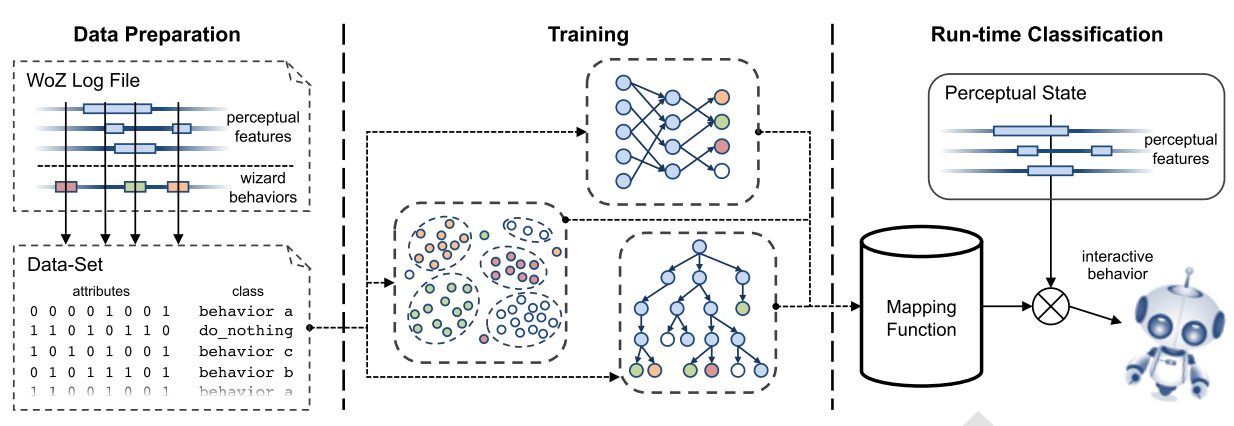
\includegraphics[width=\textwidth]{images/RestrictedPerception_ML_Diagram.png}
  %\end{framed}
  	\caption{Illustration of a \ac{ML} system in a \ac{HRI} application. The dataset is collected and prepared, then it is given to a \ac{ML} algorithm, and lastly, in run-time, the mapping function returns the most appropriate response given an input. From~\cite{Sequeira2016}.}
  	\label{fig:MLDiagram}
\end{figure}
\vspace{-3mm}

Finally, the predictive models' performance are tested using data that were not used during the training stage (test set and training set respectively). In order to limit overfitting issues, model validation techniques such as cross validation are used to test if the classifier is sufficiently generic to any given independent test dataset.

Usually, in supervised learning, the performance is measured regarding the precision (Equation~\ref{eqn:precision}) and recall (Equation~\ref{eqn:Recall}) of the generated output according to the what is expected in the corpus (TP, FP, and FN stands for True Positives, False Positives, and False Negatives, respectively).

\vspace{-9mm}
\begin{multicols}{2}
	\begin{equation}
		Precision = \frac{TP}{TP + FP}
		\label{eqn:precision}
	\end{equation}\break
	\begin{equation}
		Recall = \frac{TP}{TP + FN}
		\label{eqn:Recall}
	\end{equation}
\end{multicols}
\subsection{Reinforcement Learning}
\label{subsec:ReinforcementLearning}

\acf{RL} is sub-field in \ac{ML} that guides agents' actions, in an environment, to maximise a cumulative reward~\cite{Sutton:1998:IRL:551283, Dayan1992}. \ac{RL} systems contain:

\begin{itemize}
	\item A set of possible world states $S$;
	\item A set of possible actions $A$;
	\item Transitioning rules between states;
	\item A immediate reward function $R(s,s',a)$ with $a \in A$, and $s,s' \in S$;
	\item Rules to describe the environment.
\end{itemize}

Typically, these systems deal with environments where the optimal reward function might not be clear~\cite{Sutton:1998:IRL:551283}. To tackle this issue, \ac{RL} agents uses exploration strategies to find the best policy function $\pi(s)$ that returns the most probable action $a \in A$, given a state $s \in S$, that maximises the cumulative reward (Equation~\ref{eq:policy}). In social behaviours, agents that are eager to interact with its partner (instead of being silent) will acquire more information regarding it's performance during interactions and will be able to learn more quickly as they test new different interactional strategies.

\vspace{-3mm}
\begin{equation}
	\pi(s) = a,\,a \in A\, and\,s \in S
	\label{eq:policy}
\end{equation}

One well researched \ac{RL} algorithm is Q-Learning~\cite{Dayan1992}. In Q-Learning, the virtual agents learns and stores Q-Values that depends on the reward value for a given action $R(s_t,a_t,s_{t+1})$, on an estimation of future reward $\max_{a}Q(s_{t+1},a)$, on the learning rate $\alpha_t \in {[0,1]}$, and on the discount value $\gamma \in {[0,1]}$ (Equation~\ref{eq:QLearning}). The learning rate $\alpha_t$ defines the weight of old information during learning, and the discount value $\gamma$ defines the weight of future rewards.

\vspace{-4mm}
\begin{equation}
	Q(s_t,a_t) = (1-\alpha_t)Q(s_t,a_t) + \alpha_t\left[R(s_t,a_t,s_{t+1}) + \gamma\max_{a}Q(s_{t+1},a)\right]
	\label{eq:QLearning}
\end{equation}

The Q-Values can be zero at the beginning of the learning process, meaning that the agent's does not have previous, or, value different than zero, meaning the the agent has previous knowledge~\cite{Malfaz2011}. The values for $\alpha$ and $\gamma$ are defined according to the developed scenario, the purposes of the agents and overall quality of the final \ac{RL} model.

Lastly, there are two main issues when using \ac{RL}: identifying the reward function and gathering data to satisfy the combinatorial explosion of environment features and possible actions. To solve the first issue, authors suggest extracting the reward function from human experts during demonstrations using inverse \ac{RL}~\cite{Ng2000, Thomaz2006}. That is, collect feedback from human experts regarding the virtual agent's performance and use the information collected to define a reward function. To solve the second issue, the model should take into account fewer environment features and actions.
\cleardoublepage

%Chapter 3
\fancychapter{Related Work}
\label{chap:relatedwork}

This chapter presents the state of the art related to this work. Since there is a lack of rapport agent studies, the following chapter will focus on agents that are capable, to some extent, of managing rapport.

\subsection{Theoretical Models of Rapport for Agents}
\label{sub:sec:ComputationalModelsOfRapport}

Rapport is a mostly unconscious phenomenon~\cite{Zwiers2011} that occurs during interactions marked by strong perceptions of coordination, positivity and mutual attention.

The most important concepts for managing rapport are: planning social behaviours (Figure~\ref{table:BuildingRapportPlan}), learning social behaviours and flexible mechanisms to regulate current actions. Rapport models involve several complex cognitive mechanisms. Therefore it is beneficial to discretise it into smaller sets capable of, for example, enhancing positivity (friendliness) using self-disclosure or enhancing coordination and attentiveness through backchannel and turn-taking strategies~\cite{Sacks1974, Kahn2008, Welbergen2012}. The latter strategies are allied with good listeners as they must able to understand how to provide well-timed adequate feedback (backchannel) and identify appropriate moments to become the speaker (turn taking) and incite further dialogue~\cite{Sacks1974, Poppe2010}.

Zhao, Papangelis, and Cassell, propose a theoretical model to manage long-term rapport~\cite{Zhao2014, Papangelis2014} that is very relevant for current implementations of long-term social companionship agents~\cite{Lisetti2013, Bickmore2005, Kang2005}. Similarly to what was described previously in Section~\ref{subsec:Rapport}, the proposed model treats rapport as an interactional goal that is satisfied through strategies and actions according to the current state of the interaction and the user model (See Table~\ref{table:TCArchitectureDyadicRapportManagement:State}).

The strategies and the selected actions, despite initially representing the general sociocultural norms, must adapt to the interpersonal norms of the relationship and the context~\cite{Zhao2014}. As the relationship evolves, the dyadic state and the internal models should be updated in order to store the most accurate description of the interaction and return better behavioural responses that satisfy the dyad behavioural expectations~\cite{Papangelis2014}.

\vspace{-3mm}
\begin{table}[]
    \centering
    \begin{tabular}{@{}ll@{}}
        \toprule
        
        \multirow{1}{*}{\textbf{Dyadic State}} & Rapport State; Behavioural model; Friendship Status; History \\ \midrule
        \multirow{2}{*}{\textbf{User Model}} & User goals; Shared knowledge; Task model; \\  
        & Conversational Agent putative dyadic state \\ \bottomrule        

    \end{tabular}
    \caption{Relevant data structures for rapport models. Adapted from~\cite{Zhao2014}.}
    \label{table:TCArchitectureDyadicRapportManagement:State}
\end{table}
\vspace{-7mm}

Another important aspect for managing rapport is the ability to continuously adapt to the current interaction and context, give incremental feedback~\cite{Kopp2007, Zwiers2011, Reidsma2011, Visser2014}, and even recover from mistakes~\cite{Kahn2008}. Its usefulness is remarked on complex synchronised behaviours such as speech and handshakes~\cite{Zwiers2011}. This requires bidirectional connections between the behaviour realisers and the behaviour planners to enable quicker corrections~\cite{Reidsma2011}. This also requires incremental planning and execution of behavioural chunks that can be potentially interrupted, modified or even replaced~\cite{Reidsma2011, Visser2014, Kopp2007, Zwiers2011}. This approach moves away from the typical SAIBA model~\cite{Kopp2006} and requires extending the current \ac{BML}~\cite{Kopp2007, Zwiers2011, Reidsma2011} specifications.
\subsection{Creating Rapport Agents using Rule-Based Approaches}
\label{sub:sec:rulebasedAgents}

In the context of the document, we consider rule-based systems as systems that use rules implicitly or explicitly. For example, the former mimics head gestures using motion sensors and the latter generates backchannel behaviours if the conversational partner pauses his speech for more than one second. Rule-based systems are great for deterministic scenarios where the agent does not need to be as robust as other systems used in non-deterministic scenarios~\cite{Mutlu2006} where rules might not be easy to define. However, these systems are not easily ported to other scenarios, nor are they easily scalable because they are often based on non-trivial conditions~\cite{Kok2012}, and are often specifically tailored to discrete scenarios.

Mutlu et al., implemented a scripted mutual gaze agent that synchronises gaze behaviour with pre-recorded voice and gestures~\cite{Mutlu2006}. In their experience, they concluded that participants would recall the story better when the robot looked at them more. Additionally, using the same gaze frequency, women felt better when the storytelling agent gazed less at them. This is important if we want to develop agents for education scenarios where transmitting information is crucial.

Stanton et al., developed a robot assistant for a cooperative visual tracking game (the ``shell game'')~\cite{Stanton2014}. Volunteers would ask the robot for help. However, occasionally, the robot would volunteer to give an answer. In their experiment, they concluded that eye gaze can have powerful effects upon participant decision-making and behaviour, and influence their task performance. For example, humans tend to comply to the robot's suggestion when it gazed at them on harder tasks but, on easier tasks, gaze reduced trust. The authors postulates that ``robot gaze can have either a positive or negative impact upon trust and compliance, depending upon the nature of the robot’s request or suggestion''.

Andrist et al., developed a virtual agent focused on mutual-gaze behaviour in a therapy scenario~\cite{Andrist2015} that would systematically swap its gazing target between the task area and the conversational partner's using tracking sensors. According to their study, matching gaze behaviour models to the user's personality increases motivation and engagement in repetitive tasks. In other words, different personalities require different rules. For example, between tasks, when therapists would provide encouragement, introverts shift more often their gaze to the therapist than extroverts.

%Chidambaram \textit{et al.}, developed a robotic agent to study the impact of vocal and bodily cues in persuasion~\cite{Chidambaram2012} on Desert Survival Tasks~\cite{30} using gaze, gestures, vocal cues and even proximity to the user. In their findings, they concluded that the presence of non-verbal behaviours impacts people's compliance while and that vocal cues do not. However, the study was made on a hypothetical scenario and it was
\section{Creating Rapport Agent using Data-Driven Based Approaches}
\label{sec:datadrivenbasedAgents}

Rule-based systems are not easily scalable knowing that it is impossible to program an agent to handle every possible situation and outcome, especially when interacting with the unpredictability of human behaviour. Therefore, some scenarios may benefit from having agents capable of adapting to changes in the external world and generate more appropriate social behaviour using data-driven models through several \ac{ML} approaches. Despite not being used actively by this thesis systems, it is fundamental to mention current research work on this area as it is proving invaluable to create agents capable of producing more natural behavioural in comparison with simpler rule-based systems.

\subsection{Supervised Learning}
In supervised learning, the algorithms infer a function from a labelled training set that contains both the input set and the corresponding target value. 

Kok et al., developed an iterative data-driven rapport model focused on generating timings for backchannel behaviours in a dyadic conversational setting~\cite{Kok2012}, \ac{IPL}. The distinctive aspect is the usage of perceptual (subjective) evaluation to identify the moments of the interaction that are perceived as socially inappropriate. In the perceptual evaluation, multiple subjects evaluate the agent's behaviours by pressing a \textit{Yuck} button whenever they would rate each one as socially inappropriate (\ac{PCS})~\cite{Huang2010, Poppe2011}. The resulting model takes into consideration that different listeners have different personalities and that some social behaviours are not mandatory and, therefore not socially inappropriate if they do not occur. This sample retrieval contrasts with the typical corpus-based backchannel models, as in the latter the negative samples are retrieved randomly as long as they do not overlap with the positive samples marked in the corpus~\cite{Kok2012}. Following Figure~\ref{fig:ipl_system}, the typical corpus-based approach is used as the baseline~\cite{DeKok2011} (yellow area) that will be refined with every sequence of generation of behaviour (pink area), subjective evaluation (blue area) and finally training (green area). The resulting model was perceived more natural when compared with the tradition corpus-based approach, however, the authors suggest extending their work with more relevant features from rapport (e.g., mutual gaze, head angles and smiles).

\begin{figure}
	\centering
	\includegraphics[width=0.3\textwidth]{images/IPL_system.png}
	\caption{Schematic representation of the \ac{IPL} framework. From~\cite{Kok2012}.}
	\label{fig:ipl_system}
\end{figure}

\subsection{Unsupervised Learning}

In unsupervised learning, as opposed to supervised, the data does not contain the target value, therefore, the algorithms will try to cluster the data into groups regardless of their meaning.

Mohammad et al., propose a model for interactive robots that can learn how to interact naturally with human conversational partners in different environments and contexts~\cite{Mohammad2010} using unsupervised learning. One of the tested successful scenarios was learning how to apply backchannels in a dyadic setting with a human instructor. According to their results, the backchannel behaviour generation was more natural, performing better than the traditional rule-based, however, there is no comparison regarding the traditional supervised learning approaches.

\subsection{Active Learning}
In active learning, the algorithms interact to seek knowledge regarding how to classify an instance with a label~\cite{Bishop2006}.

Cakmak, Thomaz and colleagues have been researching the potential of active learning on agents that actively seek information and fill gaps in their knowledge, potentially improving their performance~\cite{Chao2010, Cakmak2010, Cakmak2012, Thomaz2006}. In their studies, they noticed that people who better understand the agent's queries are able to train the model with ``perfect accuracy relatively quickly'' and had more confidence on the trained model performance~\cite{Chao2010}. However, previous work has been more focused on learning task-related information and not, learning better interactional models to build and maintain rapport.

Moreover, it is important to properly design the experiments to correctly collect data. For example, Thomaz et al., developed an agent using reinforcement learning \cite{Thomaz2006}. During the experiment, despite asking the humans not to provide feedback (only guidance), they influenced the results. As the author describes ``people use the reward signal to give anticipatory rewards or future directed guidance for the agent''.

\subsection{\acf{WoZ}}
\label{subsec:woz}
In \acf{WoZ} studies~\cite{Steinfeld2009}, subjects are led to believe that they are interacting with an autonomous robot when, in fact, they are interacting with a human (the wizard). Following the current trend of using \ac{WoZ} studies~\cite{Steinfeld2009} to train virtual agents~\cite{Knox2014, Mutlu2006} to be more socially competent, Pedro Sequeira et. al. propose a methodology for discovering interaction strategies from restricted-perception \ac{WoZ} studies~\cite{Sequeira2016}. In restricted-perception \ac{WoZ}, the wizard's perceptions and actions are limited to the same extent as the agent enabling a better learning environment and better resemblance to the studies environment~\cite{Sequeira2016}. The set of perceptions and actions are collected using mock-up studies. The disadvantage of this approach is that it requires more preparation than the unrestricted \ac{WoZ} and, even then, it might be impossible to completely isolate the wizard's perceptions.
\section{Creating Rapport Agents using Hybrid Approaches}

Recently, researchers are exploring hybrid agents that combine the advantage of rule-based systems to define high-level interaction rules that are triggered by simpler perceptual states and data-driven models to generate behaviour according to more complex situations that may emerge during interactions.

Pedro Sequeira et. al. proposes the usage of mock-up studies and the previously mentioned restricted-perception \ac{WoZ} (Section~\ref{subsec:woz}) to develop a Hybrid Controller that takes advantage of rule-based systems and \ac{ML}-based systems in a tutoring scenario~\cite{Sequeira2016}. Following Figure~\ref{fig:RestrictedPerception_DesignProcess}, the inherent agent's limitations are defined in the \textit{Task AI} to be used on the restricted-perception \ac{WoZ} Studies. The hybrid controller is based on the expert knowledge and the \ac{WoZ} data collected during the previous stage, and is responsible for deciding when and which behaviour to trigger. For example, a rule-based component would trigger a summarisation of the main achievements during the game and another \ac{ML}-based component would trigger actions that were learnt during the restricted-perception \ac{WoZ} studies (recall that the wizards controls ``which interaction behaviour should be triggered and when to trigger it''~\cite{Sequeira2016}). In the last stage, \textit{Strategy Refinement}, \ac{HRI} researchers assess the agent's performance and refines the controller if necessary for situations that may not have been properly learned or, for situations that require more relevant information.

\begin{figure}[H]
	\centering
	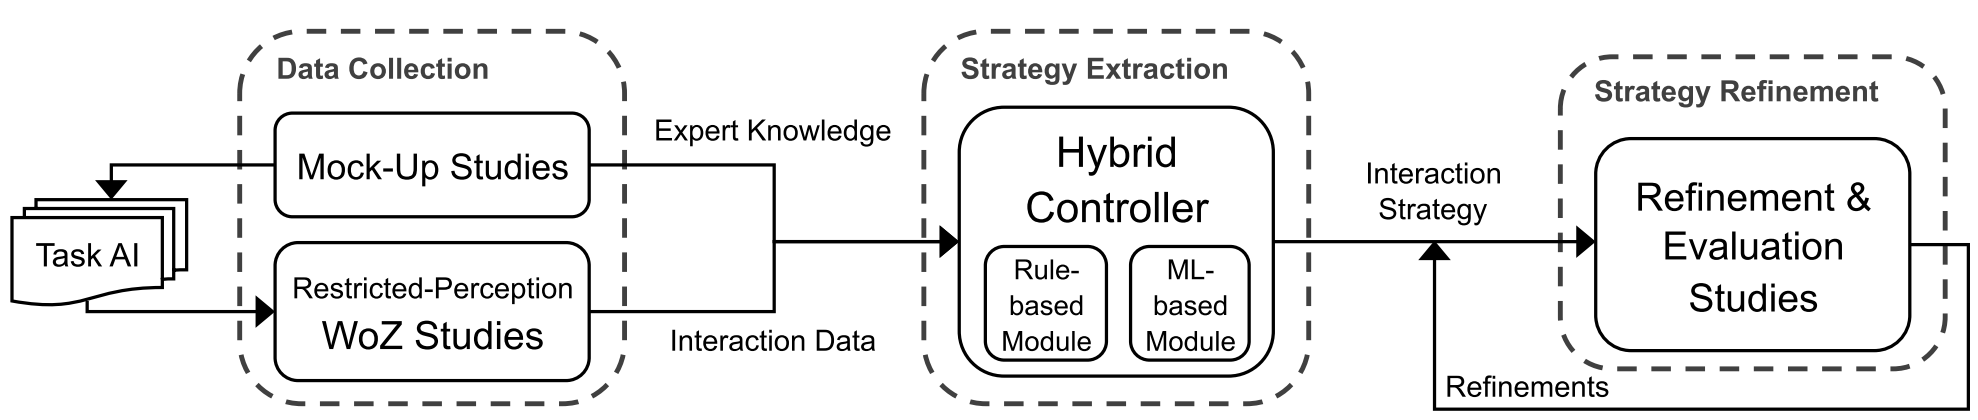
\includegraphics[width=0.85\textwidth]{images/RestrictedPerception_DesignProcess.png}
	\caption{Restricted-perception \ac{WoZ} study methodology. From~\cite{Sequeira2016}.}
	\label{fig:RestrictedPerception_DesignProcess}
\end{figure}




\subsubsection{Virtual Rapport 2.0} \hspace*{\fill} \\
\label{sub:sec:virtualrapport2}

Huang et al., developed a short-term rapport agent to enhance mutual attention and coordination using backchannels through a data-driven approach that takes into account context-specific response models in a dyadic conversational setting~\cite{Buschmeier2011}. The model determines the best suitable timings to generate specific backchannel behaviours and turn-taking opportunities according to the perceptual state observed.

%%%%%%%%%%%%%%%%%%%%%%%%%%%%%%%%%%%%%%%%%%%%%%%%%%%%%%%%%%%%%%%%%%%%%%%%%%%%%%%%%%%%%

\paragraph{\textbf{System description}}

Following Figure~\ref{fig:virtualrapport2System}, the system contains the following modules:
\begin{itemize}
	\item \textbf{\textit{Perception}}: analyses human speaker's behaviour in real time;
	\item \textbf{\textit{Response Models}}: predicts timing of backchannel feedback and end-of-turn opportunities in real time using information from the environment and from the agent itself. It also decides which behaviour to generate;
	\item \textbf{\textit{Generation}}: generates the output from the response models;	
	\item \textbf{\textit{Consensus Data}}: contains data collected from Rapport 06-07 dataset and Self-disclosure data-set (\url{http://rapport.ict.usc.edu}) using \ac{PCS}. The data contains dyadic interactions between a human speaker telling a story and human silent listener.
\end{itemize}

\begin{figure}[hbt]
  \centering
  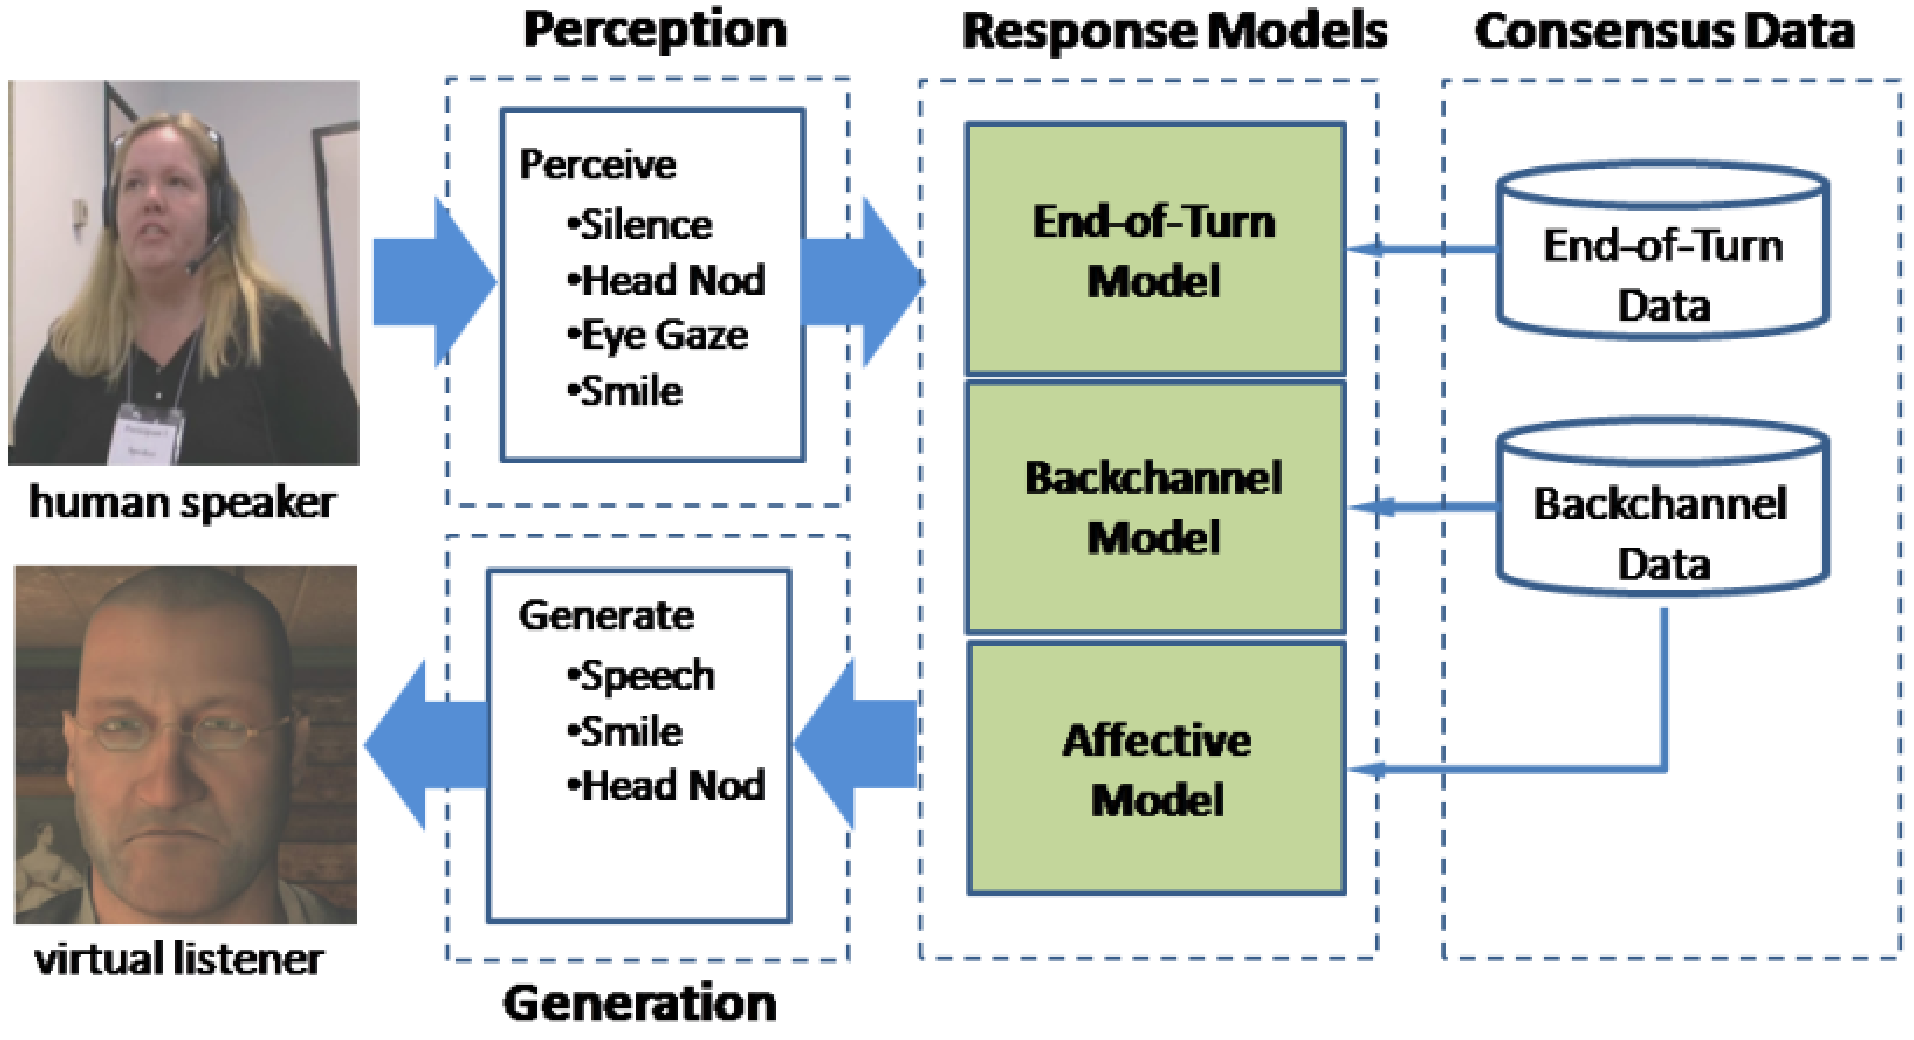
\includegraphics[width=0.8\textwidth]{images/VirtualRapport2_System.png}
  \caption{Architecture of Virtual Rapport 2.0: The \textit{Perception} module analyses human behaviour in real time. \ac{PCS} data is used to create the \textit{Response Models} module. Lastly, the output of the models is generated by the \textit{Generation} module. From~\cite{Buschmeier2011}.}
  \label{fig:virtualrapport2System}
\end{figure} 

As depicted in Figure \ref{fig:virtualrapport2System} there are three models in the \textit{Response Models} module: \textit{End-of-turn}, \textit{Backchannel}, and \textit{Affective}.

The first model, \textit{end-of-turn}, using a rule-based approach, identifies turn-taking opportunities by analysing the current speaker's non-verbal behaviours. For example, if the human interrupts the virtual agent, the agent stops, yields his turn and, says ``I am sorry, keep going'' while showing a facial expression~\cite{Buschmeier2011}.

The second model, \textit{Backchannel}, is \ac{ML}-based (using forward-only inference \ac{CRF} for real-time predictions) and trained using the Rapport 06-07 dataset. It is capable of predicting when and how to give non-verbal feedback.

The last model, \textit{Affective}, analyses facial feature points in real time and detects whenever the speaker is smiling.
 
During the interaction, the three response models are used in conjunction to decide whenever it is appropriate to generate a backchannel. If the speaker is smiling (according to the \textit{Affective} model) and if it is a good opportunity to generate a backchannel (according to the \textit{Backchannel} model) then a head nod (one of the three identified in their studies) is generated accompanied by a smile.

%%%%%%%%%%%%%%%%%%%%%%%%%%%%%%%%%%%%%%%%%%%%%%%%%%%%%%%%%%%%%%%%%%%%%%%%%%%%%%%%%%%%%%%%

\paragraph{\textbf{Evaluation}}
The developed virtual agent interacted with the human subjects in a interview environments in which the former was the interviewer and the later the interviewed. With the goal of comparing the developed system with the previous version~\cite{Gratch2006}, the evaluation measured the following dimensions: rapport (five-item social presence scale~\cite{Bailenson2001}), overall naturalness, backchannel feedback and end-of-turn prediction.


%%%%%%%%%%%%%%%%%%%%%%%%%%%%%%%%%%%%%%%%%%%%%%%%%%%%%%%%%%%%%%%%%%%%%%%%%%%%%%%%%%%%%%%%

\paragraph{\textbf{Discussion}}
The results demonstrates a significant improvement over the previous version. Over 90\% of the users preferred the Virtual Rapport 2.0 rapport agent over the previous rule-based system~\cite{Gratch2006, Morency2008}. The timing's precision and recall are much better, leading to a better synchronism and perceived naturalness from the user during the interaction. According to the authors, the data-driven design, the much richer set of emotions capable of mimicking smiles, and the generation of more natural head gestures might explain the overall better results on the stronger feelings of rapport.

To conclude the most relevant aspects of the system are:
\begin{itemize}
	\item Corpus based approach;
	\item Identification of different head nods patterns;
	\item Duality of \ac{ML}-bases decision and smile to generate backchannel behaviour;
	\item Creative strategy for handling interruptions.
\end{itemize}
\subsubsection{\acl{SAL}} \hspace*{\fill} \\
\label{subsec:AutonomousSensitiveArtificialListeners}

Schröder et al. developed a virtual agent integrated in SEMAINE~\cite{Schroder2010} called \ac{SAL} that has the required capabilities to sustain conversational dialogues and be a good listener~\cite{Schroder2012}.

\paragraph{\textbf{System Description}}

Following the representation of the \ac{SAL} system in Figure~\ref{fig:sensitiveAgent}, the most relevant components are: \textit{Feature extractors}, \textit{Analysers}, \textit{Interpreters}, \textit{Action proposers}, and \textit{Action selection}. The \textit{Feature extractors} component extracts several features such as head gestures, facial features, emotions and, most of all, acoustic features. These features are later analysed by the \textit{Analysers} and \textit{Interpreters} components. The former component analyses non-verbal behaviours and speaker's emotions to produce an estimate of the information's reliability. The later component, given the information available, returns the best state representation for the user, dialogue and agent. Following this, several \textit{Action proposers} will propose an action, in parallel, given previous information. Following, the \textit{Action selection} component selects the action with the highest estimated quality, and lastly, the \textit{Behaviour generator} generates the desired action (utterances and facial animations).

\vspace{-3mm}
\begin{figure}
	\centering
	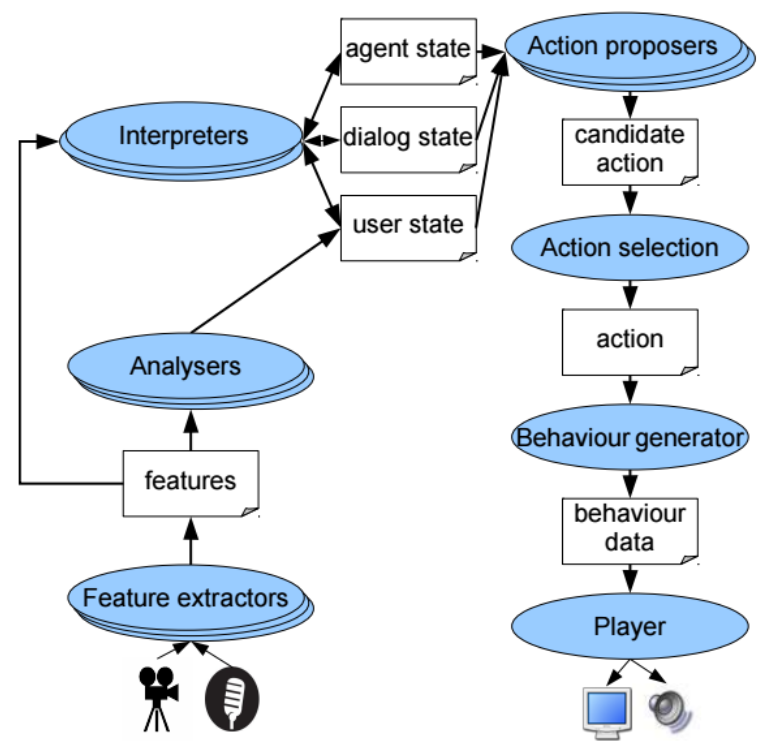
\includegraphics[width=0.5\textwidth]{images/SensitiveAgent.png}
	\caption{\acl{SAL} conceptual architecture. From~\cite{Schroder2012}.}
	\label{fig:sensitiveAgent}
\end{figure}
\vspace{-7mm}

The agent is capable of identifying whether it should be in listener or in speaker mode. This is relevant as the \textit{Action selection} component gives more priority over speaker's actions. An example speaker action would be  saying ``Well?'' or ``Go on, tell me your news!'' after a long pause. In addition, in listener mode, the \textit{Action selection} component chooses the most appropriate backchannel to be produced according to the emotions and interest level estimated from the user.

\paragraph{\textbf{Evaluation}}

The objective was to evaluate if emotion-related abilities influence the quality of human interactions. Firstly the users, with minimal \ac{HRI} experience, receive a introductory briefing on the available personalities they can interact with (4 in total). Then, they can interact twice with each available personality one with the expressive agent, the other with the affective features of the output disabled (randomly). The user interacts with the \ac{SAL} agent's presented in a computer screen (only the face is rendered), using the available cameras and microphones.

\paragraph{\textbf{Discussion}}
There is evidence that expressive abilities may substantially impact the interactions between humans and agents by denoting that flow and perceived engagement was much higher in the emotional \ac{SAL} than in the control environment. Compared with previous described systems, it is one of the most complete models for managing backchannels and turn taking strategies, however, as stated previously in Section~\ref{subsec:Rapport}, attentiveness and coordination are not enough to build rapport, it is also necessary to stimulate positivity which this system does not cover. To conclude, the most relevant aspects of the systems are:

\begin{itemize}
	\item Generate good listeners without understanding semantically what it is being said;
	\item Parallel independent action proposers that uses both rule and \ac{ML} approaches;
	\item Dedicated dialogue management models;
	\item Covers several users affective states by modelling distinct characters.
\end{itemize}
% https://www.lightbluetouchpaper.org/2007/03/14/how-not-to-write-an-abstract/
% http://web.ece.ucdavis.edu/~jowens/biberrors.html

\subsection{Overall Discussion}
\label{subsec:RelWorkDiscussion}

Developing a computational models capable of managing rapport similarly to humans is not an easy feat. Researchers had to focus their research on different aspects of rapport and assess their overall contribution. Table~\ref{fig:comparison:rapportSystems} and Table~\ref{fig:comparison:vh:systems}, respectively, compares the systems regarding how they learn social behaviours, and the used rapport management strategies.

\addtolength{\tabcolsep}{1pt}
\begin{table}
	\centering
	\begin{tabular}{lccccccccccc}
		& \textbf{Type}
		& \textbf{Agent} 
	  	& \rot[70]{\textbf{Gaze}}
	  	& \rot[70]{\textbf{Backchannel}} 
	  	& \rot[70]{\textbf{Small-Talk}} 
	  	& \rot[70]{\textbf{Facial Expressions}}
	  	& \rot[70]{\textbf{Gestures}} 
	  	& \rot[70]{\textbf{Mirroring}} 
	  	& \rot[70]{\textbf{Smile}}
	  	& \rot[70]{\textbf{Turn Taking}}
	  	& \rot[70]{\textbf{Praise}}
	  	\\
	  	\midrule
	  	%%%%%%%%%%%%%%%%%%%%%%%%%%%%%%%%%%%%%%%%%%%%%%%%%%%%%%%%%%%%%%
	  	Mutlu et al.~\cite{Mutlu2006} & Rule-based & Robotic & \cmark & \xmark & \xmark & \xmark & \xmark & \xmark & \xmark & \xmark & \xmark\\
	  	%%%%%%%%%%%%%%%%%%%%%%%%%%%%%%%%%%%%%%%%%%%%%%%%%%%%%%%%%%%%%%
	  	Stanton et al.~\cite{Stanton2014} & Rule-based & Robotic & \cmark & \xmark & \xmark & \xmark & \xmark & \xmark & \xmark & \xmark & \xmark\\
	  	%%%%%%%%%%%%%%%%%%%%%%%%%%%%%%%%%%%%%%%%%%%%%%%%%%%%%%%%%%%%%%
	  	Andrist et al.~\cite{Andrist2015} & Rule-based  & Robotic & \cmark & \xmark & \xmark & \xmark & \cmark & \xmark & \xmark & \xmark & \cmark\\
	  	%%%%%%%%%%%%%%%%%%%%%%%%%%%%%%%%%%%%%%%%%%%%%%%%%%%%%%%%%%%%%%
	  	Mohammad et al.~\cite{Mohammad2010} & \ac{ML}-based  & Robotic & \textbf{?} & \cmark & \xmark & \xmark & \xmark & \xmark & \xmark & \xmark & \xmark \\ 
	  	%%%%%%%%%%%%%%%%%%%%%%%%%%%%%%%%%%%%%%%%%%%%%%%%%%%%%%%%%%%%%%
	  	Huang et al.~\cite{Buschmeier2011} & \ac{ML}-based & Virtual & \xmark & \cmark & \cmark & \cmark & \cmark & \cmark & \cmark & \xmark & \xmark\\
	  	%%%%%%%%%%%%%%%%%%%%%%%%%%%%%%%%%%%%%%%%%%%%%%%%%%%%%%%%%%%%%%
	  	Kok et al.~\cite{Kok2012} & \ac{ML}-based & Virtual &  \xmark & \cmark & \xmark & \xmark & \cmark & \xmark & \xmark & \xmark & \xmark\\
	  	%%%%%%%%%%%%%%%%%%%%%%%%%%%%%%%%%%%%%%%%%%%%%%%%%%%%%%%%%%%%%%
	  	Schröder et al.~\cite{Schroder2012} & \ac{ML}-based & Virtual & \xmark & \cmark & \xmark & \cmark & \cmark & \xmark & \xmark & \cmark & \xmark\\
  		\bottomrule
	\end{tabular}
	\caption{Brief comparison regarding how different virtual agents manage strategies. The systems presented here appear in the same order as in the main body of the text.  \protect\cmark, \protect\xmark \, and \textbf{?}, represents whether the specified strategy is applied, not applied or unclear, respectively.}
	\label{fig:comparison:rapportSystems}
	
\end{table}
\addtolength{\tabcolsep}{-1pt}

Current literature suggests continuing the research on learning social behaviours from \ac{WoZ}~\cite{Sequeira2016, Knox2014, Papangelis2014} studies and use primarily \ac{RL}~\cite{Thomaz2006, Kok2012, Zhao2014, Papangelis2014} classifiers (Section~\ref{subsec:ReinforcementLearning}). This class of algorithms are applicable in rapport as there are sequences of states that will help the agent to know when and how backchannels should be produced in order to build rapport (the reward function). In addition, authors suggest developing solutions capable of adapting current course of actions to the current context of the interaction to improve the quality of virtual agents during interactions~\cite{Kopp2007, Zwiers2011, Reidsma2011, Visser2014}.

\begin{table}[]
	\centering
	\begin{tabular}{|l|c|c|}
		\hline
		\textbf{System}              	& \textbf{Training Source} 	& \textbf{Iterative} \\ \hline
		%%%%%%%%%%%%%%%%%%%%%%%%%%%%%%%%%%%%%%%%%%%%%%%%%%%%%%%%%%%%%%%%%%%%%%%%%%%%%%%%%%%%%%%%%%%%%%%%%
		Mohammad et al.~\cite{Mohammad2010} & Direct Samples (Unsupervised) & Yes \\ \hline
		%%%%%%%%%%%%%%%%%%%%%%%%%%%%%%%%%%%%%%%%%%%%%%%%%%%%%%%%%%%%%%%%%%%%%%%%%%%%%%%%%%%%%%%%%%%%%%%%%
		Virtual Rapport 2.0~\cite{Buschmeier2011} 			& Corpus			& No \\ \hline
		%%%%%%%%%%%%%%%%%%%%%%%%%%%%%%%%%%%%%%%%%%%%%%%%%%%%%%%%%%%%%%%%%%%%%%%%%%%%%%%%%%%%%%%%%%%%%%%%%
		\acf{IPL}~\cite{Kok2012}          				& Corpus \& Subjective evaluation			& Yes \\ \hline
		%%%%%%%%%%%%%%%%%%%%%%%%%%%%%%%%%%%%%%%%%%%%%%%%%%%%%%%%%%%%%%%%%%%%%%%%%%%%%%%%%%%%%%%%%%%%%%%%%
		\acf{SAL}~\cite{Schroder2012} & Corpus \& \ac{WoZ}		& Yes \\ \hline
		%%%%%%%%%%%%%%%%%%%%%%%%%%%%%%%%%%%%%%%%%%%%%%%%%%%%%%%%%%%%%%%%%%%%%%%%%%%%%%%%%%%%%%%%%%%%%%%%%
		Restricted Perception~\ac{WoZ}~\cite{Sequeira2016}  & \ac{WoZ}		& Yes \\ \hline
		
	\end{tabular}
	\caption{Brief comparison of methodologies to learn human social behaviours.}
	\label{fig:comparison:vh:systems}
\end{table}

Most of all, the communication goals of interactions must be considered when developing rapport agents. The context in which the communication partners will interact, the inherent limitations of the virtual agents' perceptions and actions and, most importantly, what kind of emotions and actions we want to elicit from the conversational partner are crucial for the development of such agents. For example, in tutoring applications, mutual gaze plays an important role for increased learning performance \cite{OTTESON1980, SHERWOOD1987, Fry1975}, and in negotiation scenarios not reciprocating negative self-disclosure has ben shown to destroy rapport\cite{Bronstein2012}.




\cleardoublepage

%Chapter 4
\fancychapter{A Rapport Computational Model}
\label{chap:rapportModel}

Inspired by current literature on rapport~\cite{Buschmeier2011, Spencer-Oatey2005, Zhao2014, Papangelis2014} and social agents~\cite{Zwiers2011, Reidsma2011, Riek2009, Niewiadomski2009, Andrist2014, Andrist2015, Cassell2007, Wang2009, Schroder2010, Buschmeier2011, Tullio2015}, we selected the most prominent features that allows researchers to design agents (either virtual or robotic) capable of building rapport and establish closer relationships more efficiently with humans. For example, take into account any particular information regarding either the user or the task to tailor the interaction strategies and be more effective on managing rapport with people (Section~\ref{sec:ComputationalModelsOfRapport}) and take into account that nowadays, researchers have been building hybrid systems that can bring forth the advantages of rule-based systems and data-driven systems. Therefore, it is crucial that the rapport model follows its fundamentals concepts (Chapter~\ref{chap:rapport}), follows the ideas proposed by Zhao, Papangelis and Cassel~\cite{Zhao2014, Papangelis2014} (Section~\ref{sec:ComputationalModelsOfRapport}), and that provides the flexibility to design behavioural models that can be refined independently from one another either through rule-based designs, or through data-driven designs that are growing in the research community.

For this purpose, the built rapport model has the following goals:

\begin{itemize}
    \item Build rapport following its three levels: positivity, mutual attention and coordination as rapport is more effective when they are considered simultaneously during interactions~\cite{Buschmeier2011, Spencer-Oatey2005, Zhao2014, Papangelis2014};
    \item Support dynamic interruption and replacement of actions that is vital to design agents capable of adapting its actions to the external world that is continuously changing~\cite{Reidsma2011, Visser2014, Kopp2007, Zwiers2011}. For example, stop speaking whenever the agent perceives that it another person wishes to take its turn;
    \item Permit concurrent execution of actions, that is, model agents capable of, for example, mimic facial expressions while nodding its head to show signs of attentiveness;
    \item Be sufficiently generic and customisable to tailor the agents to different embodiments and/or \ac{HRI} scenarios.
\end{itemize}

\section{Overview}

The rapport model takes into account the goal tree depicted in Figure~\ref{table:rapportModel}, for example, in order to enhance mutual attention, the agent should produce listener behaviour (backchannel) and establish gaze contact with the person. As detailed previously in Chapter~\ref{chap:rapport}, there may be other goals such as maintain of even destroy rapport that impacts the goal tree, however, this thesis focus solely on strategies for building rapport.

\begin{figure}[H]
    \centering
    %\begin{framed}
        \scalebox{0.7}{
            \begin{forest}
                [\textbf{Build Rapport}
                    [Stimulate Positivity 
                        [Self-disclosure][Motivate][Humor]]
                    [Stimulate Mutual Attention
                        [Mutual Gaze][Backchannel]]
                    [Stimulate Coordination
                        [Behavioural Mimicry
                            [Facial Expressions][Head Gestures]]
                        [Adhere To Social Norms]
                        [Backchannel]]
                ]               
            \end{forest}
        }
    %\end{framed}
    \caption{Goal tree of the rapport model. The nodes are goals and the leafs are actions.}
    \label{table:rapportModel}
\end{figure}

In order to make the agent more effective, it should adapt its interaction strategies to both the partner and the surrounding environment. For example, it would be a mistake the agent to behave differently than what the society expect of it. In addition, the agent should also be able to adapt at any time to changes of the environment, for example, it should be able to stop speaking at any time to give the turn to others to speak, possibly apologising for taking the time for doing it~\cite{Buschmeier2011}. For this purpose, the dyadic state of the interaction should be stored and used by the agent.

Following Figure~\ref{fig:rapportModel}, the rapport model has the following components:
\begin{itemize}
    \item \textbf{Dyadic State}: contains information regarding the interactional partner and the environment;
    \item \textbf{Perceptions}: perceptual information;
    \item \textbf{Rapport Effectors}: components that generate signs of rapport by proposing actions to the \textit{Rapport Controller} given the dyadic state of the interaction;
    \item \textbf{Rapport Controller}: manages the proposed actions sent by the rapport \textit{Effectors}. Conflicts may arise causing interruption and/or replacement of actions.
\end{itemize}

\begin{figure}[H]
    \centering
    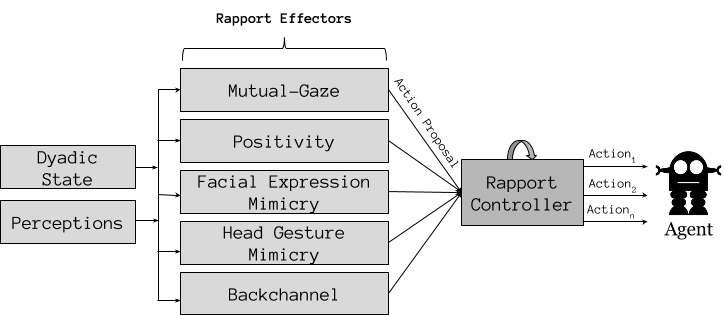
\includegraphics[width=0.9\textwidth]{images/RapportModel.png}
    \caption{Schematic representation of the rapport model.}
    \label{fig:rapportModel}
\end{figure}

The rapport \textit{Effectors} in Figure~\ref{fig:rapportModel} are independent allowing researchers to refine them separately. Additional \textit{Effectors} may be developed to complement/replace the existing ones. For example, at first, the backchannel component in Figure~\ref{fig:rapportModel} is a rule-based component that takes into account prosodic features (Section~\ref{sec:mutual_attentionModel}), however, in the future, it may be replaced by a data-driven model capable of detecting subtleties of the human behaviour more accurately.

\section{Rapport Controller}
\label{sec:rapportController}

The main responsibility of the \textit{Rapport Controller} is to manage the proposed actions sent by the different rapport strategies. Each action proposal is a quintuple $A= <G,P,E,I,T>$ containing:

\begin{itemize}
    \item \textbf{Group ($G$)}: part of agent's body that the action is attempting to manipulate. This gives more expressivity to the agent, as speaking (a \textit{Speech Group}) does not necessary interrupts a facial expression (a \textit{Face Group});
    \item \textbf{Priority ($P$ where $P \in \mathbb{N}_0$)}: relative importance of the action proposal in relation to others; 
    \item \textbf{Execution description ($E$)}: how the agent will execute the action;
    \item \textbf{Interruption description ($I$)}: how the action should be interrupted by the agent;
    \item \textbf{Timeout ($T$ where $T \in \mathbb{N}$)}: maximum duration of the action.
\end{itemize}

Concerning the management of action proposals, the controller periodically captures a snapshot of the agent's ongoing actions and pending action proposals received by the different \textit{Effectors}. Whenever a snapshot is captured or, when receiving a new action proposal, the controller analyses which actions should be interrupted (and replaced) using $I$. Following Figure~\ref{fig:no_conflicts}, as long as two action proposals have different groups ($S_G \neq A_G$), both will be executed using $S_E$ and $A_E$. However, following Figure~\ref{fig:conflict_interrupt}, in the case of a conflict ($A_{1_G}=A_{2_G}$), the action with the lowest priority is interrupted (orange area) and replaced by the newer action proposal. If the new action has lower priority than the current in execution, then it is ignored (Figure~\ref{fig:conflicting_not_interrupted}). Moreover, the action can be time limited, therefore, if the action takes longer than expected ($T$) it is interrupted, despite having higher priority.

\begin{figure}[H]
    \centering
    \begin{minipage}[b]{.4\textwidth}
        \centering
        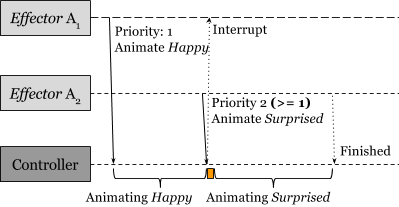
\includegraphics[width=\textwidth]{images/ConflictingAndInterrupt.png}
        \caption{Depiction of an incoming action proposal with the same \textit{Group} but with higher priority.}
        
        %The action with higher priority interrupts (orange area) and replaces the action in execution.
               
        \label{fig:conflict_interrupt}
    \end{minipage}
    \hspace{20mm}
%   \hfill
    \begin{minipage}[b]{.4\textwidth}
        \centering
        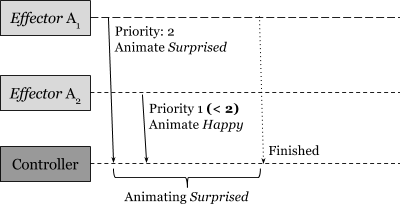
\includegraphics[width=\textwidth]{images/ConflictingNotInterrupted.png}
        \caption{Depiction of an incoming action proposal with the same \textit{Group} but with lower priority.}
        \label{fig:conflicting_not_interrupted}
    \end{minipage}
\end{figure}

%The action with lower priority is ignored as there is another action with the same \textit{Group} with higher priority is being executed.

\begin{figure}[H]
    \centering
    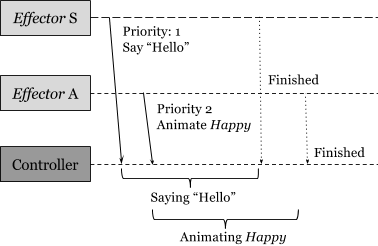
\includegraphics[width=0.4\textwidth]{images/NoConflicts.png}
    \caption{Depiction of an incoming action proposal with different \textit{Group}.}
    \label{fig:no_conflicts}
\end{figure}

%As the actions refer different \textit{Groups} there are not conflicting, and both will executed 

Lastly, the priority should be defined by the researcher. However, as rule of thumb, idle actions should have a lower priority than actions triggered by discrete states. For example, a surprise animation (as a reaction to something that just happened) should have higher priority than any idle animation.

\section{Stimulate Positivity}
\label{sub:model_positivity}

In pursuance of enhancing the first component of rapport, positivity, the Positivity \textit{Effector} takes into account the current state of the interaction to trigger, for example, contextual vocalisations to motivate or praise the interactional partner. For example, in tutoring scenarios it is important to motivate the students to achieve better results, and, more importantly, to praise them when accomplishing tough tasks. In addition, the agent should share a personal information to the person (self-disclosure), as the current literature suggests that it plays an important role in closing relationships between two strangers~\cite{Kang2011}. The interactional states and the corresponding sentences are specified by the researcher and should tailor to the dyadic state of the interaction as much as possible. For instance, in the case of the Portuguese language, which highly inflected on the gender, there have to be distinct sentences for each gender. To conclude, Table~\ref{table:positivity_rule_examples} depicts examples of interactional utterances that the researcher may specify for an agent during a game of Chess.

\begin{table}[H]
	\centering
	\begin{tabular}{|l|l|}
	\hline
	\textbf{Interactional State} & \textbf{Utterance} \\ \hline
	After Introduction & \specialcell{Did you know that I learnt the castling move yesterday where one moves\\ the king and the tower at the same time?} \\ \hline
	Player loses the queen & Don't fret, your king is still well guarded! \\ \hline
	Agent loses a bishop & Well... this could have gone better! \\ \hline
	Before the last round & These last matches were a warm-up, get ready! \\ \hline
	\end{tabular}
	\caption{Example utterances depending on the dyadic state of the interaction.}
	\label{table:positivity_rule_examples}
\end{table}

\section{Stimulate Mutual Attention}
\label{sec:mutual_attentionModel}

In order to enhance the second component of rapport, mutual attention, the model focuses on mutual gaze and listener behaviour strategies.

The Mutual-Gaze \textit{Effector} bases on the work developed by Andrist et. al.,~\cite{Andrist2015} described in Section~\ref{sub:sec:gaze}. In short, it swaps between establishing eye contact with the participant and looking at the game during pre-determined periods of time according to the following conditions: current phase of the scenario (in-task or between-tasks) and the user's personality (introverted or extroverted). By default, the lengths are the ones specified in Table~\ref{table:gazetimes} in Section~\ref{sub:sec:gaze}, however, the researcher may change these values for his specific needs (Table~\ref{table:mutualGazeParameters}). In addition, the researcher has to specify where the gaze targets on both phases (in-task and between-tasks).

%

\begin{table}[H]
	\centering
	\begin{tabular}{|l|l|l|l|c|}
	\hline
	\multicolumn{3}{|c|}{\textbf{Parameter}} & \multicolumn{1}{c|}{\textbf{Description}} & \multicolumn{1}{c|}{\textbf{Range}} \\ \hline
	\multicolumn{3}{|l|}{In-task Gaze Priority} & Gaze priority during the in-task phase & $\mathbb{N}_0$ \\ \hline
	\multicolumn{3}{|l|}{Between-tasks Gaze Priority} & Gaze priority during the between-tasks phase & $\mathbb{N}_0$ \\ \hline
	\multirow{4}{*}{Extrovert} & \multirow{2}{*}{In-task} & Face & Gaze duration & $\mathbb{N}$ \\ \cline{3-5} 
	 &  & Task & Gaze duration & $\mathbb{N}$ \\ \cline{2-5} 
	 & \multirow{2}{*}{Between-tasks} & Face & Gaze duration & $\mathbb{N}$ \\ \cline{3-5} 
	 &  & Task & Gaze duration & $\mathbb{N}$ \\ \hline
	\multirow{4}{*}{Introvert} & \multirow{2}{*}{In-task} & Face & Gaze duration & $\mathbb{N}$ \\ \cline{3-5} 
	 &  & Task & Gaze duration & $\mathbb{N}$ \\ \cline{2-5} 
	 & \multirow{2}{*}{Between-tasks} & Face & Gaze duration & $\mathbb{N}$ \\ \cline{3-5} 
	 &  & Task & Gaze duration & $\mathbb{N}$ \\ \hline
	\end{tabular}
	\caption{Available parameters and their description for the Mutual-Gaze \textit{Effector}.}
	\label{table:mutualGazeParameters}
\end{table}

The Backchannel \textit{Effector} is based on the work developed by Niewiadomski et. al. on the GRETA system~\cite{Niewiadomski2009} that analyses variations of the pitch during the interaction to produce listener behaviour (Figures~\ref{fig:lowering} to \ref{fig:risingLowering}). For simplicity, this \textit{Effector} only considers up-down head nods as listener signals, however, in the future it can consider vocalisations such as ``Hmm hmmm''. The available parameters are detailed in Table~\ref{table:backchannel}.


\begin{figure}[H] 
  \begin{minipage}[b]{0.5\linewidth}
    \centering
    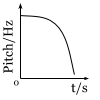
\includegraphics[width=.35\linewidth]{images/PitchLowering.png} 
    \caption{Pitch lowering when finishing a sentence disfluency.} 
    \label{fig:lowering}
    \vspace{4ex}
  \end{minipage}%%
  \hspace{3mm}
  \begin{minipage}[b]{0.5\linewidth}
    \centering
    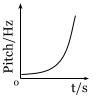
\includegraphics[width=.35\linewidth]{images/PitchRaising.png} 
    \caption{Pitch rising when asking a question disfluency.} 
    \label{fig:rising}
    \vspace{4ex}
  \end{minipage} 
  \begin{minipage}[b]{0.5\linewidth}
    \centering
    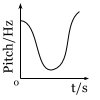
\includegraphics[width=.35\linewidth]{images/PitchLoweringRising.png} 
    \caption{Pitch lowering and rising disfluency.} 
    \label{fig:loweringRising}
    \vspace{4ex}
  \end{minipage}%% 
  \hspace{3mm}
  \begin{minipage}[b]{0.5\linewidth}
    \centering
    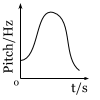
\includegraphics[width=.35\linewidth]{images/PitchRisingLowering.png} 
    \caption{Pitch rising and lowering disfluency.} 
    \label{fig:risingLowering}
    \vspace{4ex}
  \end{minipage} 
\end{figure}

\begin{table}[H]
	\centering
	\begin{tabular}{|l|l|c|}
	\hline
	\multicolumn{1}{|c|}{\textbf{Parameter}} & \textbf{Description} & \textbf{Range} \\ \hline
		Priority & Relative importance of the action proposal & $\mathbb{N}_0$ \\ \hline
		Trigger Probability & Probability of triggering mimicry behaviour & $\interval{0}{100}$ \\ \hline
		Intensity Range ($I_{min}$, $I_{max}$) & Amplitude of the head nod movement & $\interval{0}{100}$ \\ \hline
		Repetitions Range ($R_{min}$, $R_{max}$) & Number of times the agent should nod its head & $\mathbb{N}$\\ \hline
		Frequency Range ($F_{min}$, $F_{max}$) & Speed of the nod gesture & $\interval{0}{100}$ \\ \hline				
	\end{tabular}
	\caption{Available parameters and their description for the Backchannel \textit{Effector}.}
	\label{table:backchannel}
\end{table}

\section{Stimulate Coordination}
\label{sub:model_Coordination}

In order to build the third component of rapport, coordination, the model focus on behavioural mimicry, basic conformance to social norms, and backchannel (described in Section~\ref{sec:mutual_attentionModel}). Regarding behavioural mimicry, the model mimics facial expressions (e.g., happiness, surprise, and sadness) and head gestures (up-down nodes and left-right shakes).

The Facial Expression Mimicry \textit{Effector} mirrors human's unconscious facial reactions to emotions~\cite{Dimberg2000}, triggering animations according to the perceived emotion intensity $I \in \interval{0}{100}$. The model allows changing the following parameters for each type of emotion: trigger probability, minimum intensity, and priority (Table~\ref{table:facialMimicryParameters}).

%TODO a joana diz que as tabelas de Imin/Imax estão estranhas, talvez pooderia

\begin{table}[H]
	\centering
	\begin{tabular}{|l|l|c|}
	\hline
	\multicolumn{1}{|c|}{\textbf{Parameter}} & \textbf{Description} & \textbf{Range} \\ \hline
		Priority & Relative importance of the action proposal & $\mathbb{N}_0$ \\ \hline
		Minimum Intensity & Minimum threshold required to trigger mimicry behaviour & $\interval{0}{100}$\\ \hline
		Trigger Probability & Probability of triggering mimicry behaviour & $\interval{0}{1}$ \\ \hline
	\end{tabular}
	\caption{Available parameters and their description for the Facial Expression \textit{Effector}.}
	\label{table:facialMimicryParameters}
\end{table}

Head Gesture Mimicry \textit{Effector} focuses on enhancing coordination through the mimicry of head gestures such as up-down nods or shakes left-right~\cite{Riek2009, Andrist2014, Cassell2007, Wang2009}. For each type of head gesture, the model allows researchers to specify the range of the following parameters: intensity, repetitions and frequency (Table~\ref{table:headNodMimicryParameters}). Given these values, the model is able to reproduce more natural movements by randomising these parameters in each action proposal.

\begin{table}[H]
	\centering
	\begin{tabular}{|l|l|c|}
	\hline
	\multicolumn{1}{|c|}{\textbf{Parameter}} & \textbf{Description} & \textbf{Range} \\ \hline
		Priority & Relative importance of the action proposal & $\mathbb{N}_0$ \\ \hline
		Trigger Probability & Probability of triggering mimicry behaviour & $\interval{0}{100}$ \\ \hline
		Intensity Range ($I_{min}$, $I_{max}$) & Amplitude of the head-gesture movement & $\interval{0}{100}$ \\ \hline
		Repetitions Range ($R_{min}$, $R_{max}$) & Number of times the agent should produce the gesture & $\mathbb{N}$\\ \hline
		Frequency Range ($F_{min}$, $F_{max}$) & Speed of the head-gesture & $\interval{0}{100}$ \\ \hline				
	\end{tabular}
	\caption{Available parameters and their description for the Head Gesture Mimicry \textit{Effector}.}
	\label{table:headNodMimicryParameters}
\end{table}

Lastly, the agent should adhere to social norms by, for example:
\begin{itemize}
	\item Introduce itself when meeting people for the time;
	\item Greet before starting interactions;
	\item Avoid invading someone's personal space;
	\item Say ``please'' when making a request;
	\item Say ``Thank you'' when a person does a task for the agent.
\end{itemize}
\cleardoublepage

%Chapter 5
\fancychapter{Implementation of a Rapport Agent}
\label{chap:proposedapproach}

The following sections describe the implementation of the rapport model, as well as the framework that eases the development of rapport agents by both technical and non-technical researchers. The framework is built on top of the \ac{SERA} ecosystem as it provides most of the tools to translate high-level intentions into actions that can be executed by either virtual or robotic agents such \ac{EMYS} (Figure~\ref{fig:robots:EMYS2}) and NAO (Figure~\ref{fig:robots:NAO2}). The latter robot is the chosen embodiment to test the developed rapport agent.

Following this, the framework has the following goals:
\begin{enumerate}
	\item Implement the rapport model described in Chapter~\ref{chap:rapportModel};
	\item Promote re-usage of interaction strategies among different agents and \ac{HRI} scenarios;
	\item Provide non-technical researchers with the tools to customise the agent's behaviour;
	\item Provide technical researchers with the tools to develop additional rapport strategies without hindering the performance of the existing ones;	
	\item Maintain compatibility with current agents developed using the \ac{SERA} ecosystem.
\end{enumerate}

%TODO verificar following... depiction

\begin{figure}[ht]
	\centering
	\begin{minipage}[b]{.4\textwidth}
		\centering
		\frame{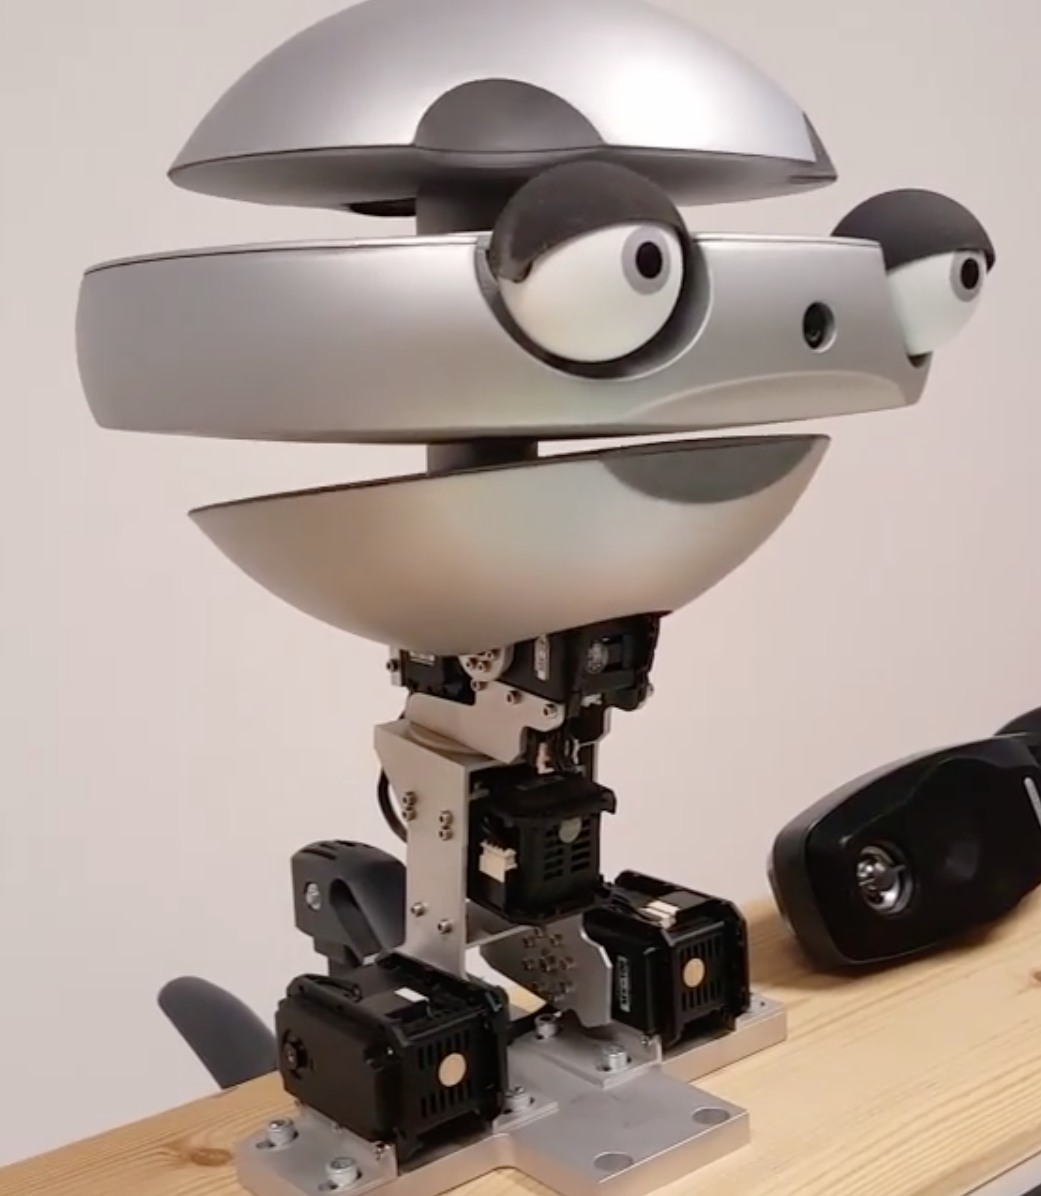
\includegraphics[width=0.4\textwidth]{images/emys.png}}
		\caption{\ac{EMYS} robot.}
		\label{fig:robots:EMYS2}
	\end{minipage}
%	\hfill
	\begin{minipage}[b]{.4\textwidth}
		\centering
		\frame{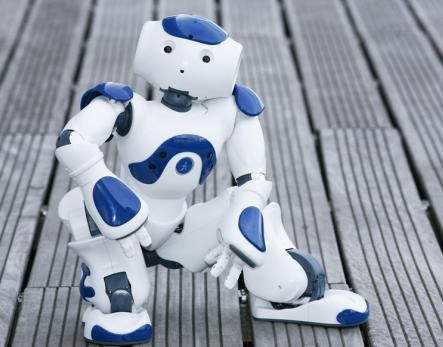
\includegraphics[width=0.55\textwidth]{images/NAO_Robot.JPG}}
		\caption{NAO robot.}
		\label{fig:robots:NAO2}
	\end{minipage}
\end{figure}



\section{\acf{SERA}: Features and Limitations}
\label{sub:sera:features_limitations}

Revisiting Section~\ref{sub:sec:SERA}, the \ac{SERA} framework is built on top of \textit{Thalamus} network, where \textit{Thalamus} clients communicate with one another through network messages. For example, \textit{Effector Thalamus} clients, in order to change agent's behaviour have to contact \textit{Skene} that processes and redirects the request to the most suitable clients: \textit{Nutty Tracks} for animations and \textit{Speech Server} for utterances. In addition, it has a finer control over the agent's action, able to, for example, causing delays or generate idle behaviour.

\ac{SERA} already assures a decoupled design for agents by using different \textit{Thalamus} clients with different responsibilities, cooperating with one another through well-defined \textit{Thalamus} network messages. Moreover, there is already support for interrupting ongoing actions, however, we need to assess how well \textit{SERA} agents are capable to quickly adapt to the dyadic state of the interaction. To this end, we ran the tests described in the following paragraphs.

In the first test, we measured the response speed between requesting an action and its execution. Following Figure~\ref{fig:solution:sera_simple_message_delay}, an \textit{Effector} \textit{Thalamus} client (in the role of a potential rapport strategy) sends an utterance request to the \textit{Skene} client. The request is dispatched and processed in \textit{Skene} and redirected to the \textit{Speech Server} which executes the desired utterance. However, each network message has to pass through \textit{Thalamus} so that it can redirect the messages to the target clients in the network. The test was successful although:

\begin{itemize}
	\item If a speech request arrives while there is one in execution, the \textit{Speech Server} executes them sequentially which can have undesired effects. For example, an \textit{Effector} may request utterance twice as a reaction to the external environment making the \textit{Speech Server} run them both twice, one after another, regardless of their duration;
	\item There is a noticeable (less than a second) delay between the requests and the effects, as requests pass firstly through \textit{Skene}, \textit{Thalamus} and finally, either \textit{Nutty Tracks} or \textit{Speech Server} (Figure~\ref{fig:solution:sera_simple_message_delay} and~\ref{fig:solution:sera_complex_message_delay}).
\end{itemize}

\begin{figure}[H]
	\centering
	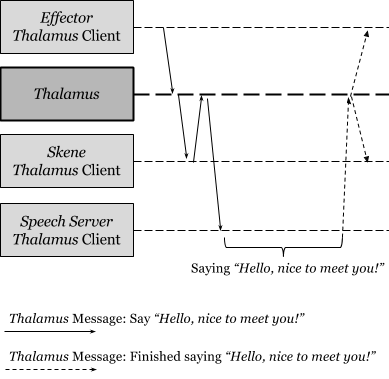
\includegraphics[width=0.45\textwidth]{images/SERA_SimpleTest.png}	
	\caption{\textit{Thalamus} network messages sent when attempting to execute a vocalisation.}
	\label{fig:solution:sera_simple_message_delay}
\end{figure}

In the second test, we extended the first test to examine the behaviour when interrupting actions (Figure~\ref{fig:solution:sera_complex_message_delay}). The sender requests an utterance to be executed, then interrupts it while it is still in execution. This test was not successful as there was a substantial delay between requesting the interruption and the effect ($\approx$ 3 seconds average in 10 tests).

\subsection*{Discussion}

We repeated the tests described in the previous section with animations instead of utterances but the results were identical. We strongly believe that the results are affected by the network nature of \ac{SERA}. When sending the messages directly from the \textit{Skene}'s \ac{GUI}, the delays were substantial shorter, reduced to less than a second, compared to the previous 3 seconds when sending from a separate client to \textit{Skene} as described in Figure~\ref{fig:solution:sera_simple_message_delay} and Figure~\ref{fig:solution:sera_complex_message_delay}.

To sum up, to accomplish our goals, taking into account \textit{Skene}'s capabilities and the tests previously described, the framework needs to:
\begin{itemize}
	\item Reduce the number of network messages that pass through the network, in order to reduce the latency between the requests and the effects, without breaking compatibility with current agents;
	\item Distribute \textit{Skene} responsibilities to different independent components in order to promote modularisation, and give the researchers the ability to customise the agent's behaviour more easily.
\end{itemize}


\begin{figure}[H]
	\centering
	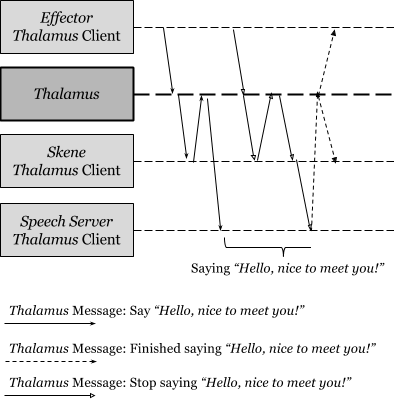
\includegraphics[width=0.45\textwidth]{images/SERA_DelayTest.png}
	\caption{\textit{Thalamus} network messages sent when attempting to execute and interrupt a vocalisation.}
	\label{fig:solution:sera_complex_message_delay}
\end{figure}

\section{Architecture Overview}

The following sections describe the framework that builds the foundations to design rapport agents using a plugin-based paradigm that takes into account the current limitations of the \ac{SERA} framework, and the rapport model detailed in Chapter~\ref{chap:rapportModel}. In order to tackle the delay between the requests and the effect (as described in Section~\ref{sub:sera:features_limitations}), the framework limits the number of network messages by communicating internally though regular method calls and events.

Following Figure~\ref{fig:rapport:archicture}, the framework contains the following elements:
\begin{itemize}
	\item \textbf{\textit{Effector Plugins}}: propose actions and enables/disables plugins;
	\item \textbf{\textit{Perceiver Plugins}}: perceive the external world and informs the interested plugins;
	\item \textbf{\textit{Utility Plugins}}: general purpose plugins that can be used to, for example, store the dyadic state of the interaction;
	\item \textbf{\textit{Rapport Controller}}: manages plugins' lifecycle, link plugin, and has the same responsibilities as the rapport model's \textit{Rapport Controller} described in Section~\ref{sec:rapportController} in Chapter~\ref{chap:rapportModel};
	\item \textbf{\textit{Thalamus Connection}}: bridges the system with \ac{SERA}, sending and receiving \textit{Thalamus} messages.
\end{itemize}

\begin{figure}[H]
	\centering
	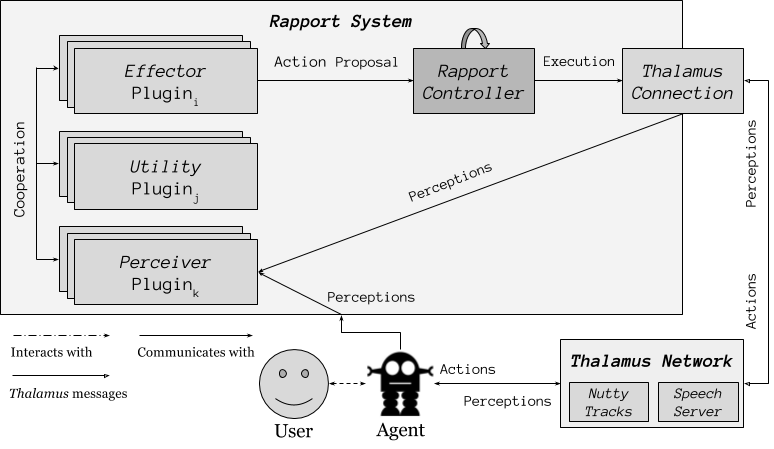
\includegraphics[width=0.9\textwidth]{images/RapportControllerArchitectureOverview.png}
	\caption{Schematic representation of the framework that implements the rapport model.}
	\label{fig:rapport:archicture}
\end{figure}

Following the same Figure~\ref{fig:rapport:archicture}, there are five types of connections:
\begin{itemize}
	\item \textbf{Perceptions}: perceptual information;
	\item \textbf{Actions}: decisive messages that trigger animations or utterances;
	\item \textbf{Action Proposal}: requests sent by \textit{Effector Plugins} that are managed by the \textit{Rapport Controller};
	\item \textbf{Execution}: set of actions triggered periodically by the \textit{Rapport Controller} - execution, interruptions or replacement according to the action proposals' stage;
	\item \textbf{Cooperation}: communication between plugins. For example, \textit{Effectors} use \textit{Perceivers} to read perceptual information and may use \textit{Utility} plugins to consult the interaction history.
\end{itemize}





\section{Rapport Controller}
\label{sec:rapportController2}

In addition to managing the agent's actions as described in the rapport model (Chapter~\ref{chap:rapportModel}), the \textit{Rapport Controller} has the following responsibilities:
\begin{itemize}
	\item Load and manage the lifecycle of the plugins;
	\item Link different plugins;
	\item Provide mechanisms to debug the proposed actions.
\end{itemize}

In the following sections, the document described how the above goals are satisfied by the developed system as well as how it aids technical and non-technical researchers the development of additional behavioural strategies, either through the development of custom plugins (Section~\ref{sec:plugins}), through customisation of specific parameters (Section~\ref{sec:plugins}), or through the definition of behaviour using markup text (Section~\ref{sub:sec:agentActionsManager}).

\subsection{Plugins Lifecycle}
\label{sub:sec:pluginLifecycle}

At the startup, the \textit{Rapport Controller} loads the available plugins from a user-selected folder (each plugin is a dynamically linked library loaded in runtime). They are all enabled by default unless specified otherwise through the configuration file that can be accessed using the controller's \ac{GUI} (Figure~\ref{fig:pluginList}). During this process, following Figure~\ref{fig:pluginLifecycle}, each plugin follows a two-step initialisation:

\begin{enumerate}
	\item \textbf{Initialisation}: initialise internal variables;
	\item \textbf{Retrieve Dependencies}: retrieve plugins that it depends on (e.g., \textit{Effectors} typically requires \textit{Perceivers}). As long as the plugin is enabled, it can be used by its peers.
\end{enumerate}

\begin{figure}[H]
	\centering
	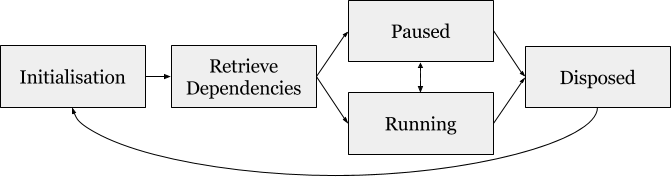
\includegraphics[width=0.7\textwidth]{images/PluginsLifecycle.png}
	\caption{\textit{Rapport Controller}'s plugin's lifecycle.}
	\label{fig:pluginLifecycle}
\end{figure}

After initialisation, the plugins can be either running or paused depending on the state of the \textit{Rapport Controller}. If the controller is running, then \textit{Perceivers} capture external world stimuli and notify the \textit{Effectors} which will attempt to modify the agent's behaviour concurrently by proposing actions asynchronously to the \textit{Rapport Controller} (perceptions events are sent asynchronously but \textit{Effectors} may pool the state of the interaction). The list of active plugins may be changed, either manually by the researcher using the provided \ac{GUI} (Figure~\ref{fig:pluginList}), either automatically by an \textit{Effector} plugin. In any case, in the case of an error in any state transition, the responsible plugin is automatically deactivated and disposed of without escalating to a sudden application crash. Finally, if an error occurs, the researcher is notified with the complete description of the fault.

\begin{figure}[H]
	\centering
	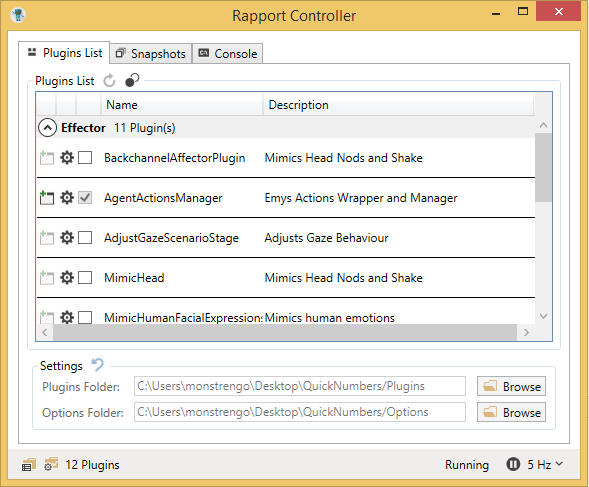
\includegraphics[width=0.6\textwidth]{images/PluginsList.png}
	\caption{\ac{GUI} representation of the list of available plugins.}
	\label{fig:pluginList}
\end{figure}

\subsection{Managing Actions}
\label{sub:sec:managingActions}

The \textit{Rapport Controller} manages action proposals as described in Section~\ref{sec:rapportController} in Chapter~\ref{chap:rapportModel}. However, in addition to the elements of action proposal quintuple $A=<G,P,E,I,T>$, the controller stores the following information:
\begin{itemize}
	\item \textbf{Status}: \textit{pending}, \textit{executing}, \textit{executed} or \textit{interrupted};
	\item \textbf{Starting time}: when the action has started executing;
	\item \textbf{\textit{Thalamus} identifier}: to monitor when actions have finished by monitoring the \textit{Thalamus} messages sent by \textit{Nutty Tracks} and \textit{Speech Server}.
\end{itemize}

The status field is required to manage the state of each action proposal. For example, following Figure~\ref{fig:actionProposalStatus}, an action proposal is only executed (using execution description $E$) as long as its previous state was \textit{pending} and, only then it can be interrupted (using the interruption description $I$). In the absence of the \textit{Thalamus} identifier, we could not flag the actions has executed, making them transition automatically to the \textit{interrupted} state. Furthermore, the controller's default frequency is 10Hz, i.e., the action proposals are analysed 10 times per second.

\begin{figure}[H]
	\centering
	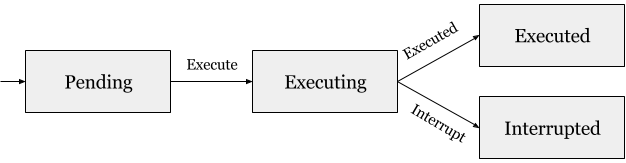
\includegraphics[width=0.6\textwidth]{images/ActionProposalCycle.png}
	\caption{Action Proposal available states and the corresponding transition graph.}
	\label{fig:actionProposalStatus}
\end{figure}

The execution and the interruption descriptions of the action proposal ($E$ and $I$, respectively) are self-contained functions specified by the researcher, therefore they can contain additional logic that is only processed when transitioning to the \textit{executing} state or to the \textit{interrupted} state, respectively. However, in order to change the agent's behaviour, they have to send the required \textit{Thalamus} messages: \textit{Speech Server} to produce utterances or \textit{Nutty Tracks} to trigger animations.

To sum up, the \textit{Effector Plugins} propose actions specifying its priority, how it should be executed, and can additionally specify how the action can be interrupted. The researcher can use the provided \ac{GUI} to debug the proposals as illustrated in Figure~\ref{fig:controllerSnapshots}. Above all, pilots are required to specify the optimal configuration of actions and their priority so that the agent's behaviour satisfies the scenario goals. 

\begin{figure}[H]
	\centering
	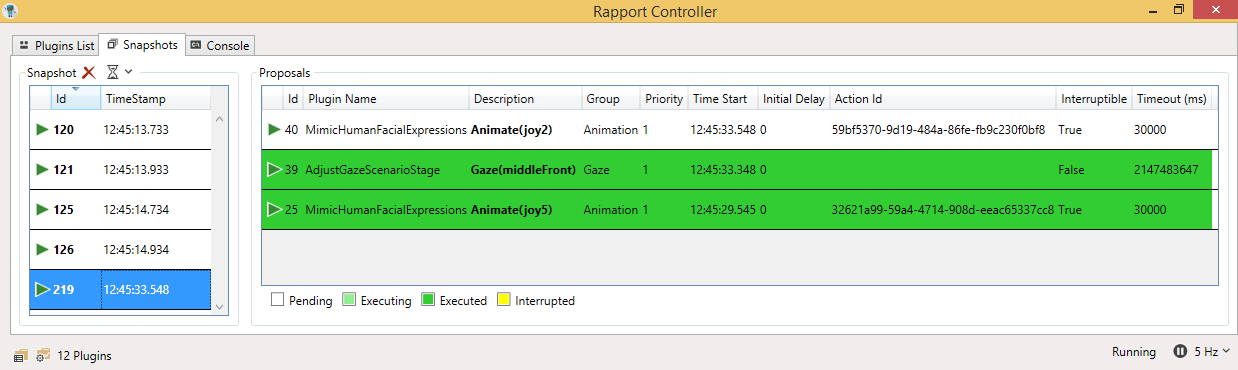
\includegraphics[width=\textwidth]{images/ScreenshotSnapshots.png}
	\caption{\ac{GUI} representation of the snapshots retrieved periodically by the \textit{Rapport Controller}.}
	\label{fig:controllerSnapshots}
\end{figure}
\section{Plugins}
\label{sec:plugins}

There are three types of plugins: \textit{Effectors}, \textit{Perceivers}, and \textit{Utility}. Their responsibility is to propose actions, to receive external world stimuli and support its peers, respectively. For the developers, the \textit{Effectors} are the only ones capable of proposing actions and changing the status of other plugins, the remaining types are identical, only differing by its name.

Furthermore, one of the goals of this project is to provide the developers with the flexibility to reuse their components on different scenarios with little to no additional effort. For this purpose, researchers only need to focus on the essentials components of the plugin as the system already provides the tools to handle, for example, optional \ac{GUI} and, more importantly, configuration files to change the rapport \textit{Effectors}' parameters specified throughout Chapter~\ref{chap:rapportModel}. The configuration file is a \ac{XML} document that is loaded during the plugin's initialisation, and can be modified afterwards (and saved) in runtime by accessing the configuration file (Listing~\ref{lst:facialExpressionsSettings} in Appendix B) by clicking on the settings icon depicted on each row in Figure~\ref{fig:pluginList}. The major advantage is that the developer does not need to recompile the plugins just to make this change. Lastly, the plugin's \ac{GUI} can be opened from the controller's user interface (Figure~\ref{fig:pluginList}). An \textit{Effector} that mimics facial expression is listed in Listing~\ref{lst:facialExpressionsSourceCode} in Appendix C.

\subsection{Effector}
\label{sub:sec:effectorPlugin}

%One could argue that another \textit{Effector} could lock the Face Action Group with an empty action with higher priority, however, this is an elaborate solution that adds unnecessary complexity to the system. An easier solution is to, track the current gaze target, and deactivate and enable the \textit{Effectors} that rely on direct eye contact.

The main task of the \textit{Effectors} was described previously in Section~\ref{sub:sec:managingActions}. However, during development, we identified a key use case that greatly impacts interactions. During the development of the scenario described in Chapter~\ref{chap:userstudies}, we identified that it would be helpful if we could deactivate and enable plugins in runtime, allowing specific rapport strategies to only affect discrete sections of the scenario. For example, deactivate idle behaviour if the agent is attentive to the task. This mechanism should be handled by a separate higher-level plugin that maps the agent's state to the list of enabled rapport strategies, leaving the essential to the \textit{Effector}.

Another key issue that emerged was internal conflict within the \textit{Effector} where it would interrupt himself repeatedly. For example, during the initial stages, the behavioural mimicry rapport \textit{Effectors} from the rapport model, described in Section~\ref{sub:model_Coordination}, were interrupting themselves regularly because the \textit{Perceiver} was continuously notifying them. To solve this issue, we added, transparently to the developer, a mechanism to track internally the proposed actions, and an additional parameter that specifies the minimum interval of time between action proposals. The researcher can choose on of the following levels:

\begin{itemize}
	\item \textbf{Unrestricted}: the \textit{Effector} must explicitly manage its proposed actions;
	\item \textbf{One Action Globally}: the \textit{Effector} cannot interrupt itself unless with a proposal with higher priority;
	\item \textbf{One Action Per Group}: same as \textit{One Action Globally} but granulated to the \textit{Group}.
\end{itemize}

In short, the task greatly influences how the different plugins will have to cooperate with one another in order to satisfy the behavioural goals of the interaction. For example, it is crucial to properly define the priority of the action proposals as it is fundamental to manage which actions will be triggered and which actions will be interrupted at any given time. To recall the reader, behaviours triggered by singular events should have higher priorities than events that happen commonly. For example, a surprise emotion (an emotion typically raised by an unexpected sudden event) should have higher priority than, for example, a happy facial expression that is at the moment mimicking the interactional partner emotion.

\subsection{Agent Actions Manager}
\label{sub:sec:agentActionsManager}

%Mencionar que é este o plugin que tem a Thalamus Connection para executar acções

Agent Actions Manager is a \textit{Utility} plugin with the following goals:
\begin{itemize}
	\item Monitors agent's actions to notify the \textit{Rapport Controller};
	\item Provide convenient wrappers for common action proposals, describing both execution and interruption descriptions ($E$ and $I$): animations, utterances, vocalisations, sounds, head nods, head shakes, and gaze;
	\item Provide non-technical researchers with the tools to change the agent's behaviour given the dyadic state of the interaction, without worrying about implementation details.
\end{itemize}

The first objective is achieved by monitoring the messages that both \textit{Speech Server} and \textit{Nutty Tracks} send to the \textit{Thalamus Network}, and compare the actions' identifiers with the stored ones. They both notify whenever their actions have started or have finished, therefore this plugin just monitors those messages containing the action \texttt{id} and redirects them to the \textit{Rapport Controller}. The second objective aims to reduce the amount of code required to specify common action proposals. Therefore, the \textit{Effectors}, in order to use the provided tools, have to request the \textit{Rapport Controller}, the Agent Actions Manager \textit{Utility} plugin during the \textit{Initialise dependencies} stage of the initialisation (Figure~\ref{fig:pluginLifecycle} in Section~\ref{sub:sec:pluginLifecycle}).

\begin{figure}[H]
	\centering
	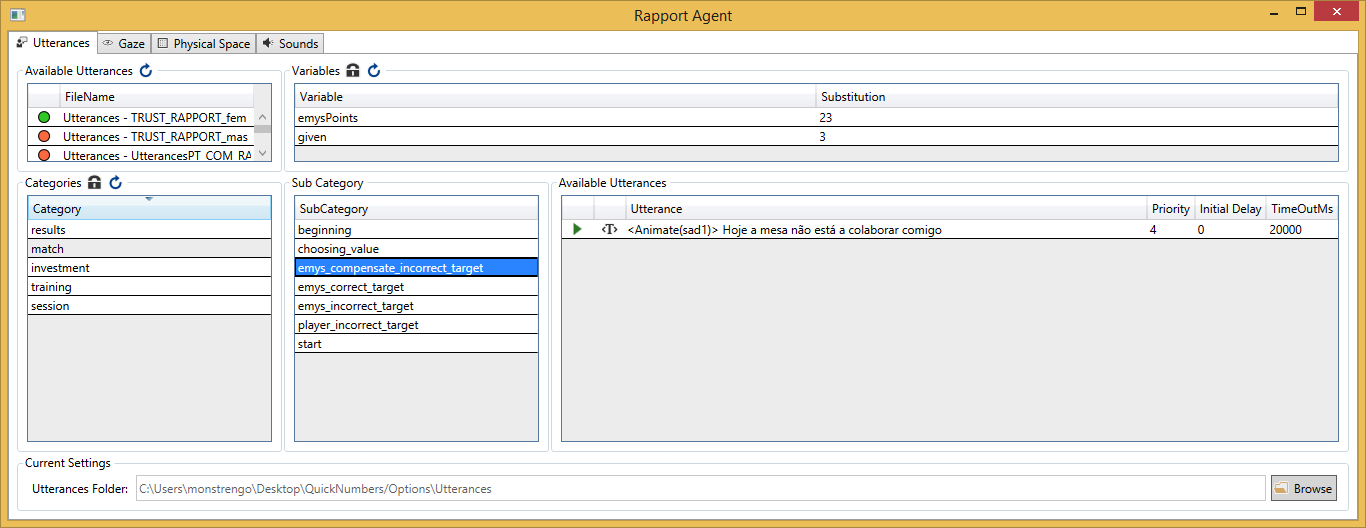
\includegraphics[width=\textwidth]{images/ScreenshotAgentsManager.png}
	\caption{\ac{GUI} representation of the Agent Action Manager \textit{Utility} plugin.}
	\label{fig:agentActionsManagerScreenshot}
\end{figure}

To accomplish the last goal, the Agent Actions Manager \textit{Utility} plugin, similar to \textit{Skene}, provides a \ac{GUI} that provides non-technical researchers with the tools to collaboratively change the agent's behavioural rules or utterances (Figure~\ref{fig:agentActionsManagerScreenshot}). However, these utterances take advantage of the prioritisation mechanism defined in the rapport model in Chapter~\ref{chap:rapportModel}. For this purpose, following Expression~\ref{eq:behaviour} and Table~\ref{fig:extended:utterances}, researchers can provide the following optional parameters: priority, delay, and timeout. These parameters will default to, the utterance priority, 0 and the utterance's timeout, respectively. 

\begin{equation}
	<action(arg_1, arg_2, ..., arg_n, [priority], [delay], [timeout])>
	\label{eq:behaviour}
\end{equation}

Similar to \textit{Skene}, the set of utterances can be imported from a \ac{CSV} file (using the format specified in Appendix D) and edited directly in the \ac{GUI}. Moreover, the developer may specify substitution variables by adding $|Variable|$ to the content of the utterance. The values of these substitution variables can be defined in the \ac{GUI} or in runtime by the \textit{Effectors}. If there are multiple variables with the same identifier, the ones provided by the \textit{Effector} will override the ones specified in the \ac{GUI}. Lastly, if there are multiple utterances for the same category and subcategory, only one is selected randomly as long as it was not selected in the past.

\begin{table}[H]
	\centering
	\begin{tabular}{|l|l|l|l|l|l|}
	\hline
	\multicolumn{1}{|c|}{\textbf{Category}} & \multicolumn{1}{c|}{\textbf{Subcategory}} & \textbf{Utterance}                                                                                      & \textbf{Priority} & \textbf{Delay (ms)} & \textbf{Timeout (ms)} \\ \hline	
	intro & greet & \specialcell{Hi $|$\textit{Name}$|$!$<$gaze(person)$>$} & 2 & 0 & 30000 \\ \hline
	game & score & \specialcell{Yey!$<$Animate(surprise2,3)$>$} & 2 & 0 & 30000 \\ \hline
	game & results & \specialcell{Managed $|$\texttt{Points}$|$!\\$<$gaze(person,3,500,5000)$>$} & 2 & 0 & 30000 \\ \hline
	end & ending & \specialcell{Thank you for your participation!\\$<$animate(happy4,4,1000)$>$} & 3 & 0 & 30000 \\ \hline		
	\end{tabular}
	\caption{Set of utterances compatible with the framework. Set of utterances compatible with \acf{SERA}. Actions are delimited by $<$ and $>$, and substitution variables by $|$.}
	\label{fig:extended:utterances}
\end{table}




%The \ac{GUI} (Figure~\ref{fig:agentActionsManagerScreenshot}) was done from scratch as the \textit{Rapport Controller} uses a more recent technology, \ac{WPF}.
\section{Rapport \textit{Effectors} Implementation}
\label{sec:rapportStrategies}

The following section describes the most relevant implementation details of the rapport \textit{Effectors} of the model detailed in Chapter~\ref{chap:rapportModel}. As denoted in Sections~\ref{sub:model_positivity}, \ref{sub:model_Coordination}, and \ref{sec:mutual_attentionModel}, the rapport strategies have to be parametrisable, so that researchers may adapt the model to any agent embodiment or \ac{HRI} scenario. 

The Positivity rapport \textit{Effector} (that satisfies the ``Stimulate positivity'' goal) and the ``Adhere to Social Norms'' goal are implemented by triggering utterances given the perceptual information of the scenario. Finally, The \textit{Effectors} were implemented and tested using robot \ac{EMYS} (Figure~\ref{fig:robots:EMYS2}).


%TODO referir que a positivity e o adhere to social norms são implementados scenario based

%In the following sections we will describe the supporting technologies, \ac{SSI}~\cite{Wagner2013}, SHORE~\cite{Ruf2011}, and GRETA~\cite{Niewiadomski2009} in Section~\ref{sec:supportingTechnologies}, followed by a brief description of the \textit{Effectors} described above.

%Most of all, in order to build rapport more effectively, one should take into consideration if the above-mentioned strategies fit the study scenario, and if they are adequate to the person the agent is interacting with (e.g., introvert and extrovert people should be handled differently~\cite{Andrist2015}). This aspect is more relevant for enhancing positivity which is mostly built either through vocal interactions or through gestures. For this purpose, in order to build positivity, the developer must build their own \textit{Effector} or \textit{Effectors}.



% Bull1981, Baxter2014
% Impact on users behaviour
%Buschmeier2011, Zhao2014, Reidsma2011, Gratch2006, Mutlu2006, Andrist2015, Stanton2014,


\subsection{Supporting Technologies}
\label{sec:supportingTechnologies}

Revisiting the rapport model described throughout Chapter~\ref{chap:rapportModel}, the rapport \textit{Effectors} require the following perceptual capabilities:
\begin{itemize}
	\item Monitor the interaction activity, for the Positivity \textit{Effectors}.
	\item Identify human emotions, and head-gestures for the behavioural mimicry \textit{Effectors};
	\item Identify speech disfluencies (Figures~\ref{fig:lowering} to \ref{fig:risingLowering}) for the backchannel \textit{Effector};
	\item Identify the user's gender and monitor the current state of the interaction, for the Mutual-Gaze \textit{Effector};
\end{itemize}

Following Figure~\ref{fig:SupportingTechnologiesOverview}, the system uses \ac{SSI}~\footnote{\url{http://hcm-lab.de/projects/ssi/}} to recognise social-signals in real-time from microphones and video feeds~\cite{Wagner2013}. \ac{SSI} uses SHORE~\cite{Ruf2011} and openSMILE~\cite{Eyben:2013:RDO:2502081.2502224} to recognise emotions, and extract prosody features, respectively. For example, \ac{SSI} identifies head-gestures using a Kinect Camera, and SHORE outputs the different emotion intensities given the video feed. Finally, \ac{SSI} periodically collects and sends the perceptual information in \ac{XML} format through network messages to other processes using ActiveMQ~\footnote{\url{http://activemq.apache.org/}}, specifically GRETA\textsuperscript{PP}.

\begin{figure}[H]
	\centering
	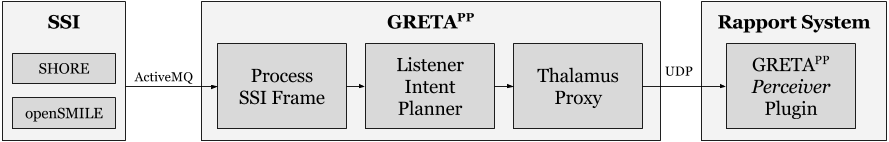
\includegraphics[width=0.95\textwidth]{images/SupportingTechnologiesOverview.png}
	\caption{Schematic representation of the components that supports the rapport model.}
	\label{fig:SupportingTechnologiesOverview}
\end{figure}

GRETA\textsuperscript{PP} is a variation of the GRETA system~\cite{Niewiadomski2009} that uses only the  \textit{Listener Intention Planner} component of the original GRETA (Figure~\ref{fig:GretaOriginal}), as we are not interested in the remaining components for the scope of this thesis. In short, GRETA\textsuperscript{PP} attempts to match the perceptual information to the first behavioural rule defined in a configuration file loaded at launch as exampled in Listing~\ref{lst:exampleGretaRule}. In the case of a match, the system might output a response signal given the response probability specified by the same rule. The original set of rules was reduced, as they were tailored for a virtual agent with different capabilities than the robot \ac{EMYS}, for example, the virtual agent is capable of moving his eyebrows and specific lip positions. Finally, taking advantage that GRETA is already integrated with \ac{SSI}, we adapted \ac{SSI} and GRETA\textsuperscript{PP} to redirect head gestures and facial expressions perceptual information to our system. It is important to mention that there is a slight delay beginning from \ac{SSI} and ending in the \textit{Perceiver}, and that only the emotion with the highest intensity is sent. The major bottleneck of the system relies on \ac{SSI} itself which is resource intensive and, in order to be able to test the system, the refresh rate had to be reduced to 5Hz which is half the default value.


\begin{lstlisting}[caption={One of the backchannels rules used GRETA and GRETA\textsuperscript{PP}.},label={lst:exampleGretaRule},language=XML]
<rule name="trigger-rise-fall">
	<usersignals>
		<usersignal id="1" name="rise_fall" modality="speech"/>
	</usersignals>
	<backchannels probability="1.0" priority="2">
		<response_reactive probability="0.4"/>
	</backchannels>
</rule>
\end{lstlisting}

Lastly, the communication with the rapport system is accomplished using \ac{UDP} sockets to transmit information in real-time without concerning with packet-loss as the system runs locally. The GRETA\textsuperscript{PP} \textit{Perceiver} Plugin, given the perceptual information, will notify the interested \textit{Effectors}.

\begin{figure}[H]
	\centering
	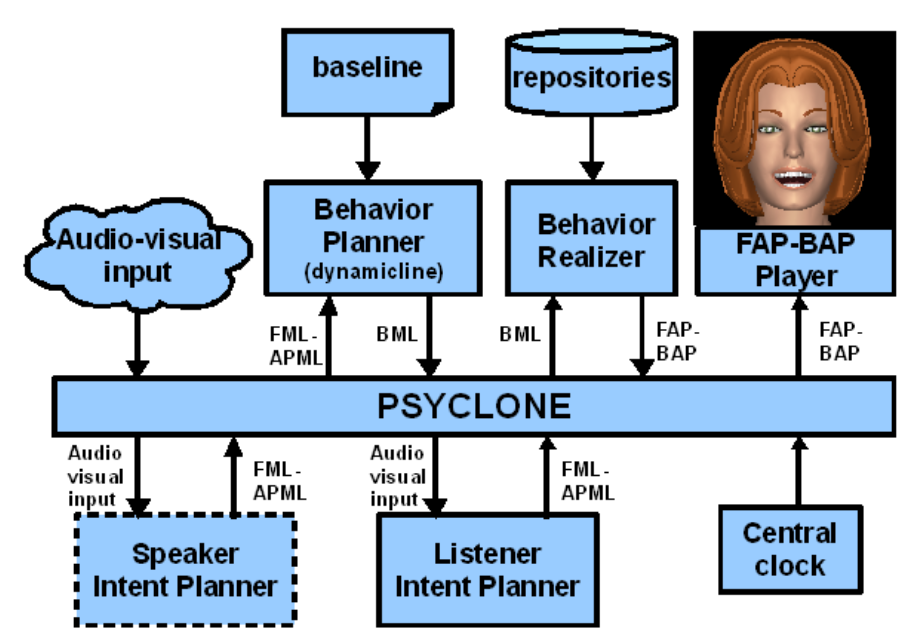
\includegraphics[width=0.6\textwidth]{images/GretaArchitecture.png}
	\caption{GRETA architecture. From~\cite{Niewiadomski2009}}
	\label{fig:GretaOriginal}
\end{figure}



% there are four main modules  that supports the rapport strategies:
%\begin{itemize}
%	\item \textbf{\ac{SSI}}: recognise social signals in realtime;
%	\item \textbf{SHORE}: recognise emotions from a video feed;
%	\item \textbf{GRETA\textsuperscript{PP}}: adapted version of GRETA~\cite{Niewiadomski2009} to generate listener behaviour;
%	\item \textbf{GRETA \textit{Perceiver} Plugin}: proxy between GRETA\textsuperscript{PP} and the \textit{Rapport Controller}.
%\end{itemize}


\subsection{Facial Expression Mimicry}
\label{sub:sec:FacialExpressionMimicry}

The Facial Expression Mimicry rapport \textit{Effector} mimics the user's emotion given the perceptual information returned from SHORE (the source code is available in listing~\ref{lst:facialExpressionsSourceCode} in Appendix C). The \textit{Effector}'s parameters (Table~\ref{table:facialMimicryParameters}) were attributed empirically following several pilots that were run with 3 different people until a balance was found between overeagerness and lack of liveness (Table~\ref{table:facialMimicryParametersValues}). In particular, the probability and the minimum delay specified in Table~\ref{table:facialMimicryParametersValues} were crucial to avoid triggering animations one, after another, for the duration of the emotion. In addition, the final \textit{Nutty Tracks} animation identifier is the base identifier followed by a random number between 1 and 5, for example, \textit{sadness1}, \textit{joy4}, and \textit{surprise3}. With this randomisation, the agent will not be as repetitive which may impact negatively the user's opinion of it. %Lastly, Anger is not specified as SHORE often mistakes it for happiness.

Nonetheless, the implementation of this plugin is not without issues as:
\begin{itemize}
    \item In absence of faces, SHORE outputs happiness emotions with a high level of intensity ($>$ 75);
    \item There is a slight noticeable delay (less than 1 second) between the emotion appearing on the video feed and being transmitted to GRETA;
    \item Camera distance and light conditions have the greatest impact on accuracy.
\end{itemize}

The issues lied on a balance between accuracy and speed. Applying a smoothing filter solved the second issue by reducing the signal spikes but it increased the delay from at most 1 second to 3 seconds. In the end, we opted to remove the smoothing filter, compensating with enabling/disabling this plugin only when required in runtime (Section~\ref{sub:sec:effectorPlugin}). Finally, the last issue is easily solved by taking the lightning conditions into consideration when preparing the physical space.

\begin{table}[H]
	\centering
	\begin{tabular}{|l|c|c|c|}
	\hline
	\multicolumn{1}{|c|}{\textbf{Parameter}} & \textbf{Happiness} & \textbf{Sadness} & \textbf{Surprise} \\ \hline
		Priority & 1 & 1 & 1 \\ \hline
		Minimum Intensity & 0.65 & 0.65 & 0.5 \\ \hline
		Trigger Probability & 0.48 & 0.48 & 0.48 \\ \thickhline
		\textit{Nutty Tracks} Base Animation & joy & sadness & surprise \\ \hline
		Minimum delay between mimicry behaviours (ms) & 3500 & 3500 & 3500 \\ \hline	
	\end{tabular}
	\caption{Parametrisation of the Facial Expression Mimicry rapport \textit{Effector}. }
	\label{table:facialMimicryParametersValues}
\end{table}


\subsection{Head Gesture Mimicry}
\label{sub:sec:HeadNodMimicry}

The Head Gesture Mimicry rapport \textit{Effector} mimics up-down nod gestures and left-right head shakes given the perceptual information returned from \ac{SSI}. In order to make \ac{EMYS} mimic head gestures, we added head nods and head shakes animations to \textit{Nutty Tracks} that takes into account the \textit{Effector} parameters specified in Table~\ref{table:headNodMimicryParameters}. The \textit{Effector} parameters were attributed empirically similar to Facial Expression Mimicry \textit{Effector} (Table~\ref{table:headGesturesMimicryParametersValues}), however, as the sensors seldom detected head gestures during the pilot tests, both gestures' probabilities were set to 1, that is, the agent will always mimic the behaviour.

Lastly, similarly to Facial Expression Mimicry \textit{Effector}, there is an apparent latency between the user's action and the mimicry behaviour, that is only solved by increasing the computational resources.

\begin{table}[H]
	\centering
	\begin{tabular}{|l|c|c|}
	\hline
	\multicolumn{1}{|c|}{\textbf{Parameter}} & \textbf{Up-Down Nods} & \textbf{Left-Right Shakes} \\ \hline
		Priority & 1 & 1 \\ \hline
		Trigger Probability & 1 & 1 \\ \hline
		Intensity Range ($I_{min}$, $I_{max}$) & (10,20) & (40,60) \\ \hline
		Repetitions Range ($R_{min}$, $R_{max}$) & (2,2) & (2,2)\\ \hline
		Frequency Range ($F_{min}$, $F_{max}$) &  (40,55) & (40,55)\\ \thickhline		
		Minimum delay between mimicry behaviours (ms) & 3500 & 3500 \\ \hline		
	\end{tabular}
	\caption{Parametrisation of the Head Gesture Mimicry rapport \textit{Effector}.}
	\label{table:headGesturesMimicryParametersValues}
\end{table}
\subsection{Mutual Gaze}
\label{sub:sec:GazeFace}

The Mutual-Gaze rapport \textit{Effector}, as described in Section~\ref{sec:mutual_attentionModel}, swaps the gaze target depending on the user's personality and on the current state of the interaction, more precisely, whenever the agent is in an in-task phase, or in a between-task phase. As we not know the personality of the user beforehand, the \textit{Effector} assumes that the interactional partner is extroverted (which has lower standard deviation than introvert following Table~\ref{table:gazetimes}). This \textit{Effector} plugin uses the rapport model's default durations parameters which are represented in Table~\ref{table:mutualGazeParametersValues}. Finally, the gaze targets identifiers depicted on the same table are known by \textit{Skene} who triggers the appropriate animations on \textit{Nutty Tracks}.

\begin{table}[H]
	\centering
	\begin{tabular}{|l|c|c|}
	\hline
	\multicolumn{2}{|c|}{\textbf{Parameter}} & \textbf{Value} \\ \hline
	\multicolumn{2}{|l|}{In-task Gaze Priority} & 1 \\ \hline
	\multicolumn{2}{|l|}{Between-tasks Gaze Priority} & 1 \\ \hline
	\multirow{2}{*}{In-task} & Face & 2660 \\ \cline{2-3} 
	 & Task & 4040 \\ \hline
	\multirow{2}{*}{Between-tasks} & Face & 3910 \\ \cline{2-3} 
	 & Task & 1010 \\ \thickhline
	\multicolumn{2}{|l|}{Face Gaze Target Identifier} & middleFront \\ \hline
	\multicolumn{2}{|l|}{Task Gaze Target Identifier} & bottomFront \\ \hline
	\end{tabular}
	\caption{Parametrisation of the Mutual Gaze rapport \textit{Effector}.}
	\label{table:mutualGazeParametersValues}
\end{table}

%Despite SHORE being capable of estimating accurately the gender of the user, it must be defined beforehand by the developer. 








%table:mutualGazeParameters
%table:backchannel
%table:headNodMimicryParameters


\subsection{Backchannel}
\label{sub:sec:backchannel}

The Backchannel rapport \textit{Effector} is based on the work developed on the GRETA system~\cite{Niewiadomski2009}, that analyses the variations of the pitch perceived by the openSMILE component of \ac{SSI}. Given the backchannel timings received from the GRETA\textsuperscript{PP} \textit{Perceiver} plugin, the \textit{Effector} plugin produces only head nods, as we were not able to generate a convincing \textit{Hmm hmmm} with a similar pitch as the generated voice by the \textit{Speech Server}. Ideally, the agent would alternate between head nods, \textit{Hmm hmmm} vocalisations, or both head nods and vocalisations. The parameters' values are depicted in Table~\ref{table:headGesturesMimicryParametersValues}, which are almost identical to the ones used in the Head Gesture Mimicry \textit{Effector}, except the priority is higher as the action proposals are executed on discrete states of the interaction. The trigger probability is identical to the one used in GRETA.

Despite succeeding with the integration of \ac{SSI} and GRETA, the resulting Backchannel \textit{Effector} did not behave as expected due to environmental factors that could not be controlled without changing the agent's embodiment as:
\begin{itemize}
	\item The \ac{EMYS}'s movement are noisy;
	\item The \ac{EMYS}'s voice is played through external speakers.
\end{itemize}

We attempted to reduce the impact of these factors by:
\begin{itemize}
	\item Use directional noise-suppressing microphone;
	\item Reduce the microphone sensivity;
	\item Adapt the \ac{SSI} pipeline to increase the pitch baseline.
\end{itemize}

To conclude, despite these efforts, this \textit{Effector} did not behave as intended, therefore it was not used in the user studies in Chapter~\ref{chap:userstudies}.

\begin{table}[H]
	\centering
	\begin{tabular}{|l|c|}
	\hline
	\multicolumn{1}{|c|}{\textbf{Parameter}} & \textbf{Backchannel Head Nod}\\ \hline
		Priority & 2 \\ \hline
		Trigger Probability & 0.4 \\ \hline
		Intensity Range ($I_{min}$, $I_{max}$) & (10,20) \\ \hline
		Repetitions Range ($R_{min}$, $R_{max}$) & (2,2) \\ \hline
		Frequency Range ($F_{min}$, $F_{max}$) &  (40,55) \\ \thickhline		
		Minimum delay between mimicry behaviours (ms) & 5000 \\ \hline		
	\end{tabular}
	\caption{Parametrisation of the Backchannel rapport \textit{Effector}.}
	\label{table:headGesturesMimicryParametersValues}
\end{table}

\section{Final Remarks}
During the previous sections, the document describes the system that implements the rapport model described in Chapter~\ref{chap:rapportModel} and extends the \ac{SERA} ecosystem to create robotic agents capable of managing rapport following current literature on models that tailor behavioural strategies to the dyadic state of the interaction. The presented \textit{Effectors} were developed and tested for robot \ac{EMYS} (Figure~\ref{fig:robots:EMYS2}), therefore the values described in Tables~\ref{table:facialMimicryParametersValues} to~\ref{table:headGesturesMimicryParametersValues} are tailored to this embodiment. Auxiliary plugins may have been developed by the researcher to monitor the scenario and trigger contextual utterances that will attempt to enhance positivity and build rapport.  In additional, the system aids the development of customisable plugins so that they can be easily changed by non-technical researchers such as psychiatrists whose knowledge on \ac{HRI} is crucial to building agents. Finally, and above all, pilot tests should be done so that the final set of possible actions sent by the agent are effective on satisfying the interactional goals of the scenario and manage rapport with the user.


%, and on the work developed by Huang et. al.~\ref{Buschmeier2011} on a virtual rapport agent. 
%Limited backchannel behaviours 



\cleardoublepage

%Chapter 6
\fancychapter{User Studies}
\label{chap:userstudies}

The developed rapport system was tested in collaboration with Nuno Xu, who is studying the impact of perceived task performance on trust. Using the Quick Numbers scenario (Figure~\ref{fig:quickNumbersScenario} and \ref{fig:quickNumbersScenarioCloseup}), we evaluate how both task performance and willingness would jointly affect trust, and observe its impact on rapport using robot \ac{EMYS}. This thesis focus only on the rapport aspects of the study, therefore, please consult Xu's Master's thesis for more details regarding how trust is evaluated~\cite{Xu2016}.

\begin{figure}[H]
	\centering
	\frame{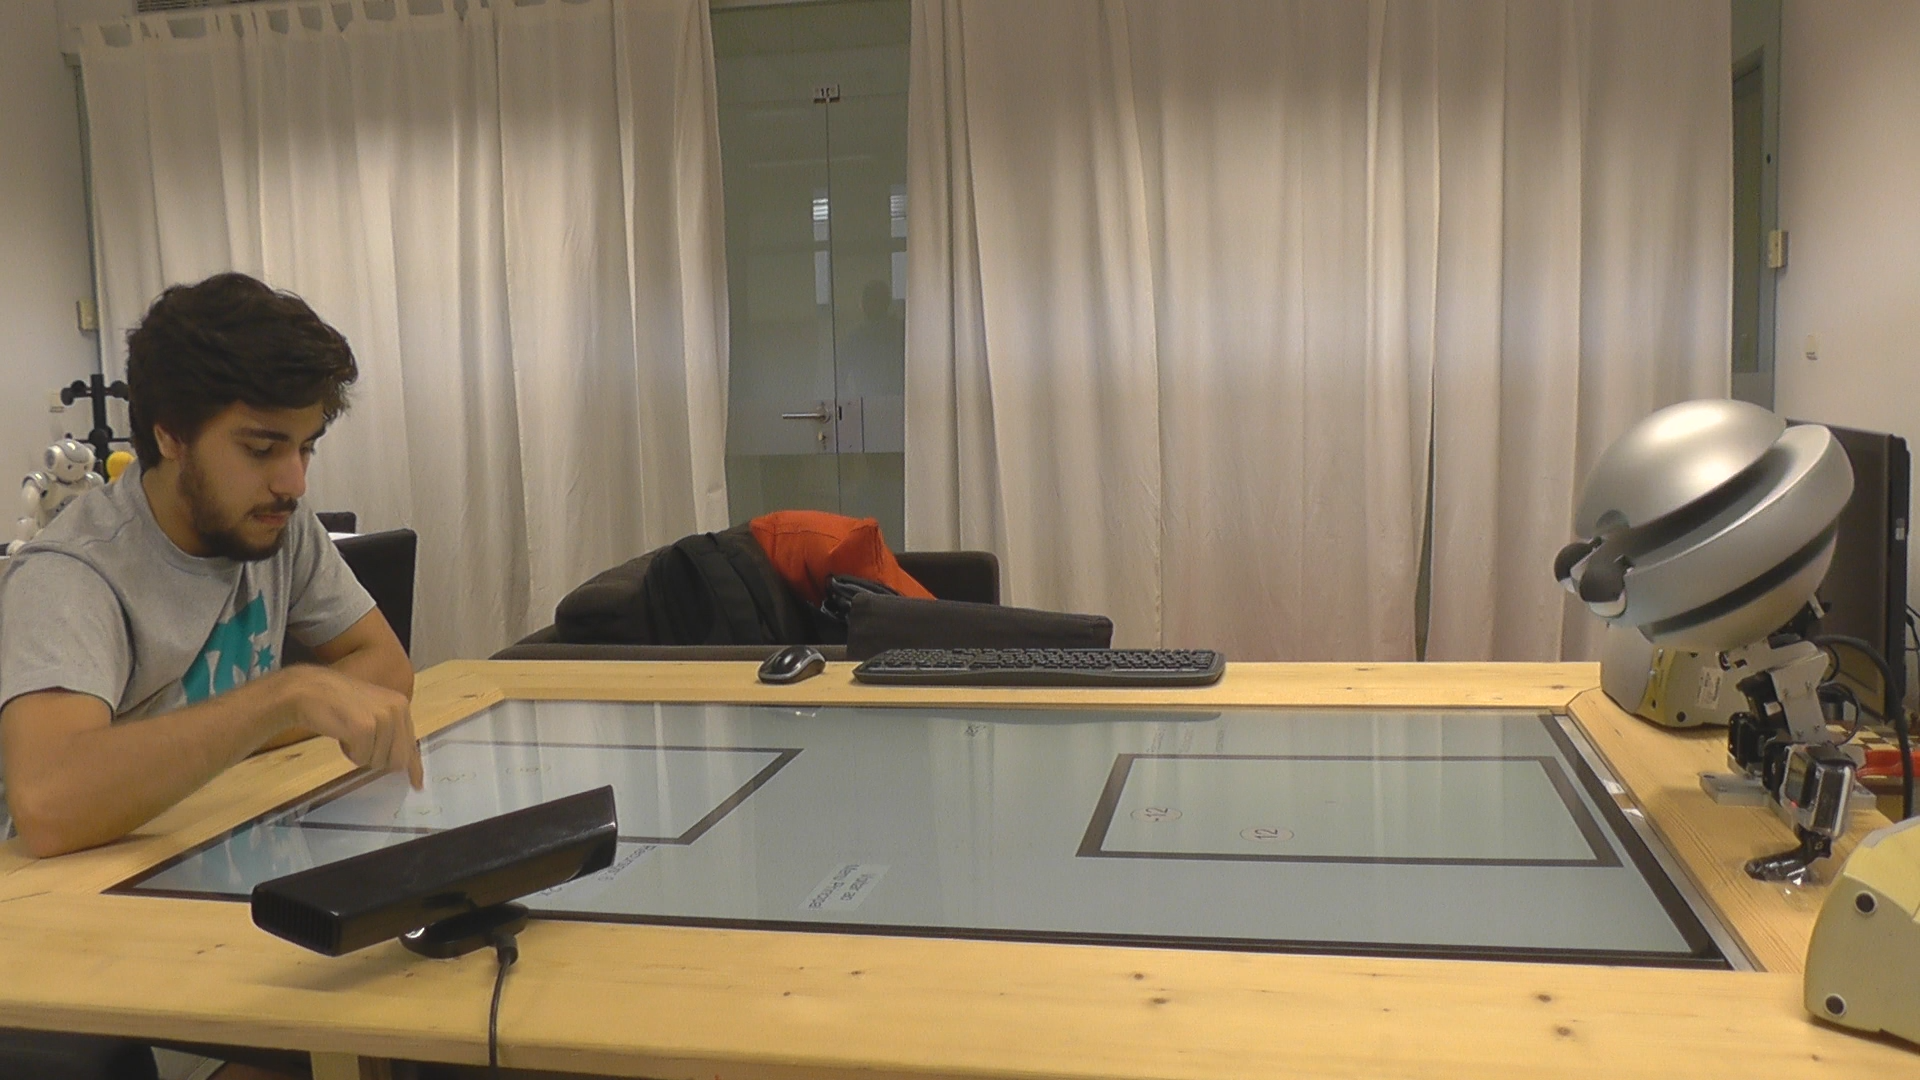
\includegraphics[width=0.7\textwidth]{images/ScenarioScreenShot.png}}
	\caption{An example of a participation in the Quick Numbers study (side view).}
	\label{fig:quickNumbersScenario}
\end{figure}

\section{Quick Numbers}
\label{sec:ScenarioDescription}

In the Quick Numbers scenario players are tasked with gaining as many resources as possible within the given time by interacting with a touch table. At the beginning, each player starts with a fixed amount of resources that can be invested before each round. Depending on the amount invested and the player's performance, the returning investment will either be greater or lesser than the investment. The task is to tap the appearing numbers in sequential order starting with number one until the end of the round (Figure~\ref{fig:quickNumbers}). With each successful tap, the score increases, and with each incorrect number, the score decreases. In the end, the resources earned are the product between the amount invested and the round's score.

In this study, \ac{EMYS} accompanies the subject throughout the scenario, not as an opponent, but as another player that is also playing the game. The scenario stages go as follow:
\begin{itemize}
	\item \textbf{Introduction}: researchers briefly explains the scenario procedures, followed by the start the scenario, where the agent starts by greeting the participant;
	\item \textbf{Training Stage}: the participant plays an informal match alone to get accustomed to the game mechanics before proceeding;
	\item \textbf{Gaming Session}: both players play a single round, at the same time;
	\item \textbf{Results Discussion}: the agent comments each player score;
	\item \textbf{Investment}: the participant is informed that he has to invest on the agent. The participant is unaware how much the agent will give in return;
	\item \textbf{Ending}: \ac{EMYS} informs the value of the investment return and thanks to the subject for his participation.	
\end{itemize}

\begin{figure}[H]
	\centering
	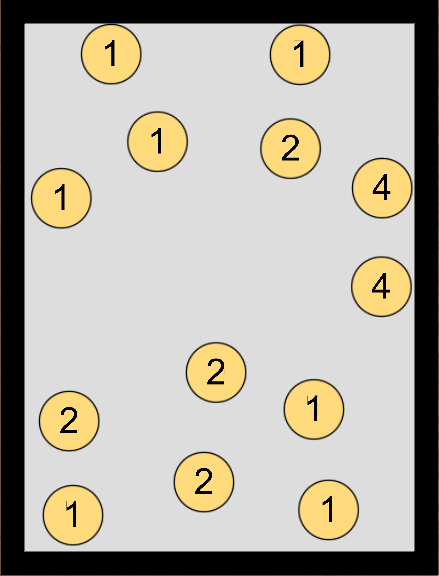
\includegraphics[width=0.3\textwidth]{images/FallingBoltsDiagram.png}
	\caption{Illustration of the Quick Numbers game developed in Unity.}
	\label{fig:quickNumbers}
\end{figure}

\section{Quick Numbers Plugins}

In addition to the plugins that implements the rapport model, we developed the following:
\begin{itemize}
	\item \textbf{Scenario \textit{Perceiver}}: monitors the scenario through \textit{Thalamus}, notifying the interested \textit{Effectors} regarding the current state of the scenario. For example, it notifies \textit{Effectors} whenever the participant tapped the correct number;
	\item \textbf{Utterances Manager}: proposes utterances according to the dyadic state of the interaction;
	\item \textbf{Rapport Strategies Manager}: enables/disables the rapport \textit{Effectors} given the current state of the interaction; 
\end{itemize}

\subsection{Utterances Manager}

This \textit{Effector} implements the positivity and the coordination component of the rapport model as it proposes utterances (in Portuguese) according to the dyadic state of the interaction following the same structure as Table~\ref{fig:extended:utterances} (Appendix D). In addition, the agent greets and dismisses properly at the beginning and at the end of the interaction, respectively, however, the rapport agent is friendlier. For example, as detailed in rapport model (Chapter~\ref{chap:rapportModel}), the rapport agent shares a personal information when introducing itself, and will motivate or praise the agent's performance. Furthermore, and more importantly, given that the participant speaks Portuguese, \ac{EMYS} will adapt his utterances according to the participant's gender. To sum up, the rapport agent:

\begin{itemize}
	\item Shares a personal information when introducing itself - ``Did you know I played Sueca recently?''~\cite{correia2016trust};
	\item Is friendlier and more comprehensive by motivating and praising the participant's performance - ``You are doing great!'', ``Don't worry, I also had a rough start'';
	\item Shows embarrassment when hitting the wrong number - ``Today's not my day'';
	\item Attempts to be humorous - ``I just finished. I won't go anywhere... how could I? I am just a head...''.
\end{itemize}

Appendix D contains the full list of the utterances used in conditions C and R for male participants.

\subsection{Rapport Strategies Manager}

The Rapport Strategies Manager \textit{Effector} defines which rapport strategies are active given the current stage of the scenario. For example, following Table~\ref{table:enabledPlugins}, it disables postural mimicry and mutual gaze rapport strategies when \ac{EMYS} participates in Quick Numbers as a player and not as a spectator. In particular, it disables Facial Expression Mimicry \textit{Effector} in the investment phase because the participant's face is not visible on the video feed (Section~\ref{sub:sec:FacialExpressionMimicry}).

\begin{table}[H]
	\centering
	\begin{tabular}{|l|c|c|c|}
	\hline
	\multicolumn{1}{|c|}{\textbf{Scenario Stage}} & \textbf{Facial Expression Mimicry} & \textbf{Head Gesture Mimicry} & \textbf{Mutual-Gaze} \\ \hline
	Introduction & \cmark & \cmark & \cmark (Between-tasks) \\ \hline
	Training Stage & \cmark & \cmark & \cmark (In-tasks) \\ \hline
	Gaming Session & \xmark & \xmark & \xmark \\ \hline
	Results Discussion & \cmark & \cmark & \cmark (Between-tasks) \\ \hline
	Investment & \xmark & \xmark & \xmark \\ \hline
	Ending & \cmark & \cmark & \cmark (Between-tasks) \\ \hline
	\end{tabular}
	\caption{Rapport strategies presence throughout the different stages of the Quick Numbers scenario.}
	\label{table:enabledPlugins}
\end{table}

\section{Methodologies and Procedures}
\label{sec:methodsAndProcedures}

In order to study the impact of the three components of rapport on users using a robotic agent we conducted a between-subjects study using the Quick Numbers scenario, following two conditions:

\begin{itemize}
	\item \textbf{Condition C:} the agent does not attempt to build rapport;
	\item \textbf{Condition R:} the agent attempts to build rapport using the rapport model described in Chapter~\ref{chap:rapportModel}.
\end{itemize}

In addition, as the study was conducted in collaboration with Nuno Xu, we had two additional conditions that are outside of the scope of this dissertation:
\begin{itemize}
	\item \textbf{Condition T:} the agent does not attempt to build rapport but attempts to build trust~\cite{Xu2016};
	\item \textbf{Condition RT:} the agent attempts to build rapport and trust with the participant~\cite{Xu2016}.
\end{itemize}

In conditions C and R, the return value is always the agent's score multiplied by the participant's investment value, but this fact is unknown to the participant. In addition, the agent's \ac{AI} that plays the Quick Numbers game is identical in every condition. Specifically, the \ac{AI}'s performance was designed so that it had a reaction time of 0.3 seconds~\cite{Boot2008} and an accuracy of 70\% (empirically chosen value), so that the agent's does not perform necessary better than the participant which could make him frustrated.

Each participant answered the questionnaire available in Appendix A that is divided into three parts: the first part is answered before the participant interacts with \ac{EMYS}; the second part is filled during the investment stage while \ac{EMYS} plays alone; the last part is filled at the end of the scenario. The first questionnaire asks demographic information and if the participant had interacted with \ac{EMYS} in the past. The first and the second part aims to gather information regarding trust~\cite{carrington2007toward, schaefer2013perception}. The third part collects information to understand the participant's opinion regarding likeability, intelligence, and animacy using the Godspeed series~\cite{bartneck2009measurement, lehmann2015good} and 6-item scales (1 means low perception and 6 the highest level of perception). In addition, this part collects the participant's perception of proximity that we are attempting to increase by building rapport~\cite{aron1992inclusion} using a 7-item scale question (1 means that the participant did not feel close to the agent and 7 means that he felt very close).

Lastly, the user study sessions were individual and performed in an isolated room accompanied only by the researcher, and lasted between 20 and 30 minutes. The sessions were recorded using two cameras: one captured the participant from the front (Figure~\ref{fig:quickNumbersScenarioCloseup}) and the other captured the both \ac{EMYS} and the user (Figure~\ref{fig:quickNumbersScenario}).

\section{Sample Description}
\label{sec:sample}

A group of 40 participants from different universities campus were included in this study. The participants were equally selected and randomly distributed between the control condition (C) and the rapport condition (R). Condition C has a mean age of 23.5±1, equal distribution of genders, and over 55\% of the participants already interacted with \ac{EMYS}. Condition R has a mean age of 25.65±3.945, 60\% male and only 25\% of the sample played with \ac{EMYS} in the past.

\section{Results}

The main goal of the agent is to build rapport, therefore we raised the following hypothesis:
\begin{itemize}
	\item Are the rapport strategies effective in making agents more likeable?
	\item Does the developed system improve agent's liveness?
	\item Do rapport strategies affect perceived intelligence?
	\item Are the rapport strategies effective in establishing closer relationships between humans and agents?
\end{itemize}

All statistical analyses further mentioned used a significance level ($sig$) of 5\%.

%TODO PREP TALK
%In the attempt of answering these questions we will look compare the obtained results from the participants on both conditions. In addition to analysing the significance level, we will assess if there is a pattern that can be confi of the The results take into account both the significance level onto the significance level between the the control condition (C) and the rapport condition (R), and we will analyse
%In order to answer the first three questions, we used the information gathered from Godspeed questionnaires~\cite{bartneck2009measurement}, and the last from proximity questions~\cite{lehmann2015good, aron1992inclusion}. The document will firstly answer the above questions, ending with a brief discussion of the results.

\subsection*{\textit{Are the rapport strategies effective in making agents more likeable?}}

In order to infer a conclusion about this questions, we compared the likeability statistics between the control condition (Figure~\ref{fig:likeability_baseline}) and the rapport condition (Figure~\ref{fig:likeability_rapport}). As the distributions do not follow a normal distribution on both conditions ($sig_C=0.001$ and $sig_R=0$), and the groups are independent, we analyse the results using the \textit{Mann–Whitney U} statistical test. As the histogram's shapes are dissimilar ($sig=0.201$), we can only compare the mean scores: 5.0±0.649 and 5.3±0.865, on conditions C and R, respectively.

\begin{figure}[H]
	\centering
	\begin{minipage}[b]{.45\textwidth}
		\centering
		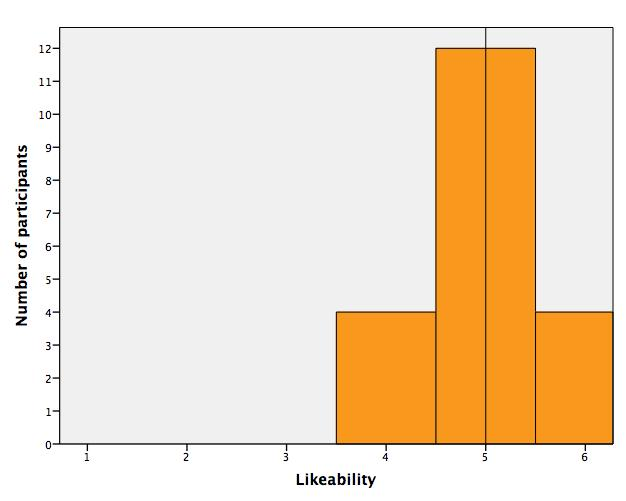
\includegraphics[width=\textwidth]{images/LikabilityBaseline.jpeg}
		\caption{Likeability histogram in the control condition. The vertical reference line marks the mean average of 5.0±0.649.}
		\label{fig:likeability_baseline}
	\end{minipage}
	\hfill
	\begin{minipage}[b]{.45\textwidth}
		\centering
		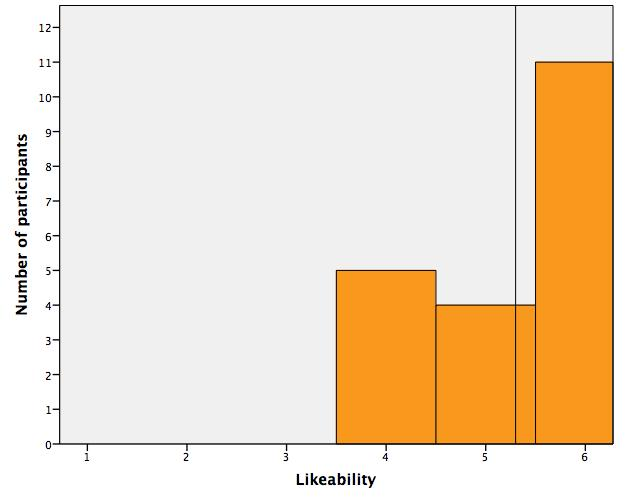
\includegraphics[width=\textwidth]{images/LikabilityRapport.jpeg}
		\caption{Likeability histogram in the rapport condition. The vertical reference line marks the mean average of 5.3±0.865.}
		\label{fig:likeability_rapport}
	\end{minipage}
\end{figure}

\textbf{Answer}: Despite the greater man average on the rapport condition, there is no statistical proof that rapport strategies are effective on increasing likeability. However, given that the mode (most frequent value) changed from 5 to 6, from condition C to condition R, we can postulate that, if we increase the sample size, we might obtain a clear confirmation that the rapport strategies affect the agent's likeability.

\subsection*{\textit{Does the developed system improve agent's liveness?}}

Similar to likeability, the animacy distribution on both conditions does not follow a normal distribution ($sig_C=0.002$ and $sig_R=0.003$), therefore we compare both conditions with the \textit{Mann–Whitney U} statistical test. The histograms are depicted in Figure~\ref{fig:animacy_baseline} and Figure~\ref{fig:animacy_rapport}, control condition and rapport condition, respectively. As the histograms' shapes are distinct ($sig=0.512$), we can only compare the mean scores: 4.25±0.716 and 4.3±1.031, on conditions C and R, respectively.

\begin{figure}[ht]
	\centering
	\begin{minipage}[b]{.45\textwidth}
		\centering
		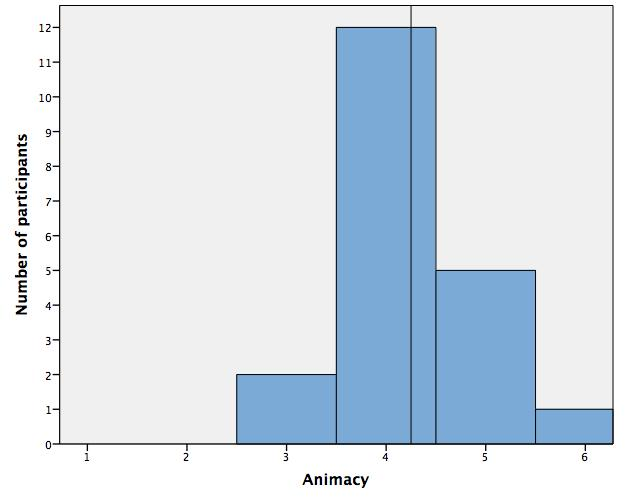
\includegraphics[width=\textwidth]{images/AnimacyBaseline.jpeg}
		\caption{Animacy histogram in the control condition. The vertical reference line marks the mean average of 4.25±0.716.}
		\label{fig:animacy_baseline}
	\end{minipage}
	\hfill
	\begin{minipage}[b]{.45\textwidth}
		\centering
		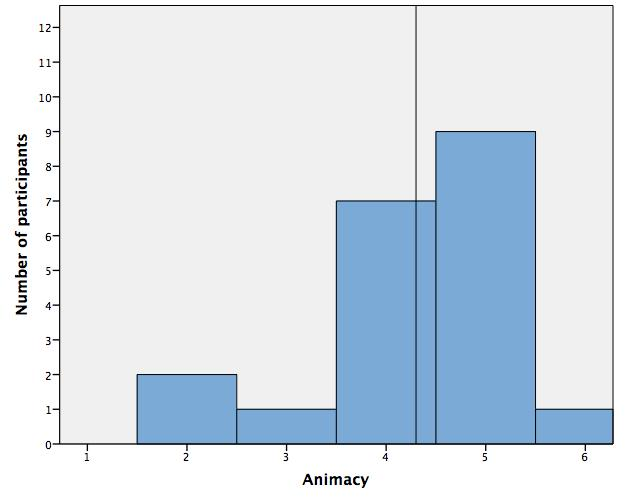
\includegraphics[width=\textwidth]{images/AnimacyRapport.jpeg}
		\caption{Animacy histogram in the rapport condition. The vertical reference line marks the mean average of 4.3±1.031.}
		\label{fig:animacy_rapport}
	\end{minipage}
\end{figure}

\textbf{Answer}: There is no definite proof that the current system improves the agent's liveness.

\subsection*{\textit{Do rapport strategies affect perceived intelligence?}}

Similar to likeability and animacy, the perceived intelligence distributions on  conditions C and R are not normal ($sig_C=0$ and $sig_R=0.002$), therefore we compare both conditions with the \textit{Mann–Whitney U} statistical test. The histograms are depicted in Figure~\ref{fig:intelligence_baseline} and Figure~\ref{fig:intelligence_rapport}, control condition and rapport condition, respectively. The histogram's shapes are dissimilar ($sig=1.0$), therefore we only compare the mean scores: 5.1±0.553 and 5.0±0.918, on conditions C and R, respectively.


\begin{figure}[H]
	\centering
	\begin{minipage}[b]{.45\textwidth}
		\centering
		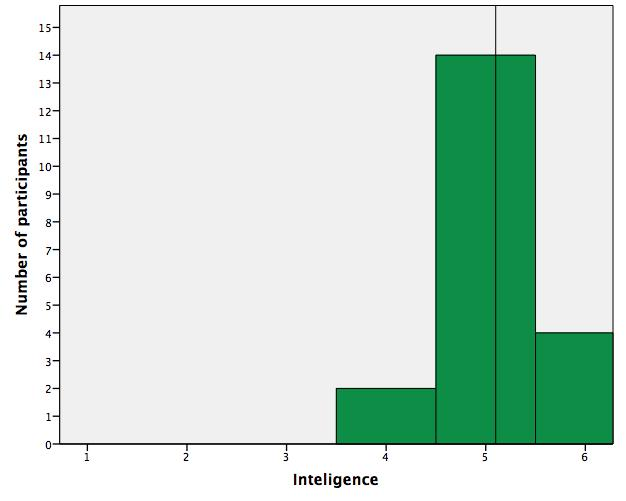
\includegraphics[width=\textwidth]{images/PerceivedIntelligenceBaseline.jpeg}
		\caption{Perceived intelligence histogram in the control condition. The vertical reference line marks the mean average of 5.1±0.553.}
		\label{fig:intelligence_baseline}
	\end{minipage}
	\hfill
	\begin{minipage}[b]{.45\textwidth}
		\centering
		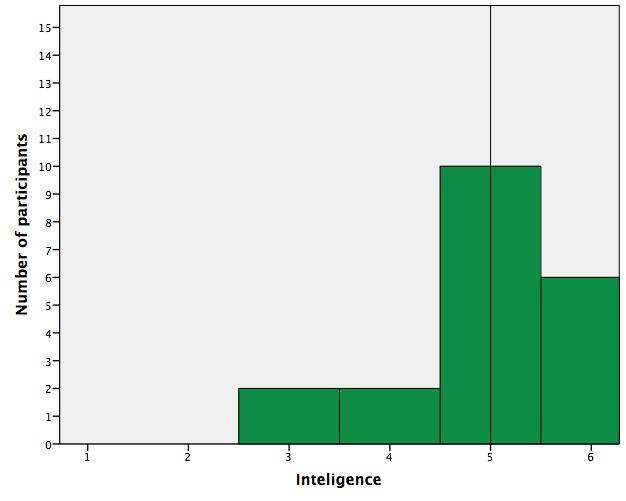
\includegraphics[width=\textwidth]{images/PerceivedIntelligenceRapport.jpeg}
		\caption{Perceived intelligence histogram in the rapport condition. The vertical reference line marks the mean average of 5.0±0.918.}
		\label{fig:intelligence_rapport}
	\end{minipage}
\end{figure}

\textbf{Answer}: There is no statistical proof that the rapport strategies have an effect on the agent's perceived intelligence.
 
\subsection*{\textit{Are the rapport strategies effective in establishing closer relationships between humans and agents?}}

In order to answer the last hypothesis, we compare the proximities answers between conditions C (Figure~\ref{fig:proximity_baseline}) and R (Figure~\ref{fig:proximity_rapport}). In both conditions, proximity follows a normal distribution ($sig_C=0.203$ and $sig_R=0.304$), therefore we use the independent \textit{t-test} statistic test which yielded the statistical significance value of 0.694 ($>0.05$), therefore we reject the null hypothesis.

\begin{figure}[H]
	\centering
	\hspace{10mm}
	\begin{minipage}[b]{.45\textwidth}
		\centering
		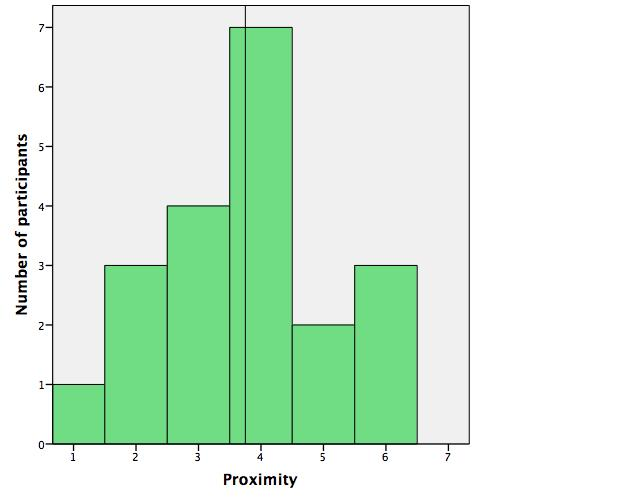
\includegraphics[width=\textwidth]{images/EmysBaseline.jpeg}
		\caption{Proximity histogram in the control condition. The vertical reference line marks the mean average of 3.75±1.410.}
		\label{fig:proximity_baseline}
	\end{minipage}
	\hfill
	\begin{minipage}[b]{.45\textwidth}
		\centering
		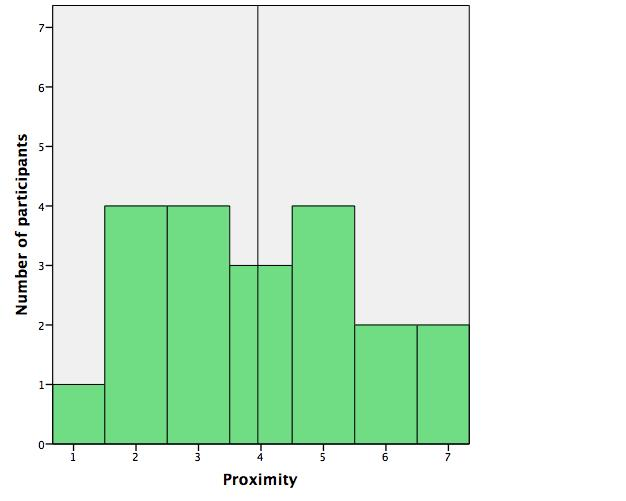
\includegraphics[width=\textwidth]{images/EmysRapport.jpeg}
		\caption{Proximity histogram in the rapport condition. The vertical reference line marks the mean average of 3.95±1.761.}
		\label{fig:proximity_rapport}
	\end{minipage}
\end{figure}

\textbf{Answer}: Despite the small increase of 0.2 on the mean score from condition C to R, the impact of the rapport strategies on proximity are inconclusive. In addition, as seen in the last bar in Figure~\ref{fig:proximity_rapport} from condition R, we had one participant that felt closest to the agent.

\section{Overall discussion}

Using mainly the subjective measures obtained from questionnaires, and given that there was no statistical significance on the obtained results, it is not possible to draw  conclusions from the experiments. However, by comparing the histograms, specially likeability’s histograms (Figure~\ref{fig:likeability_baseline} and \ref{fig:likeability_rapport}), we can infer a pattern that might lead to clear answers if we increase the sample size during future studies. Furthermore, from 1235 minutes of recorded video (using the angles illustrated in Figure~\ref{fig:quickNumbersScenario} and~\ref{fig:quickNumbersScenarioCloseup} and manual annotations during the experiments, we noticed more frequent positive reactions from the participants in the rapport condition. One one occasion, the participant remarked the agent's capability to synchronise his happy animation with its laugh. One another two independent occasions, both male and female participants flattered the agent's ability to distinguish their gender.

It is also possible to retrieve behaviour metrics by annotating (either manually or automatically) the recorded video. For example, we could compare the user's gazing behaviour between the control condition and the rapport condition, that is, compare how often the agent gazed at \ac{EMYS}. In addition, we can compare the smile frequency between both conditions using the video feed from a frontal view camera (Figure~\ref{fig:quickNumbersScenarioCloseup}).

\begin{figure}[H]
	\centering
	\frame{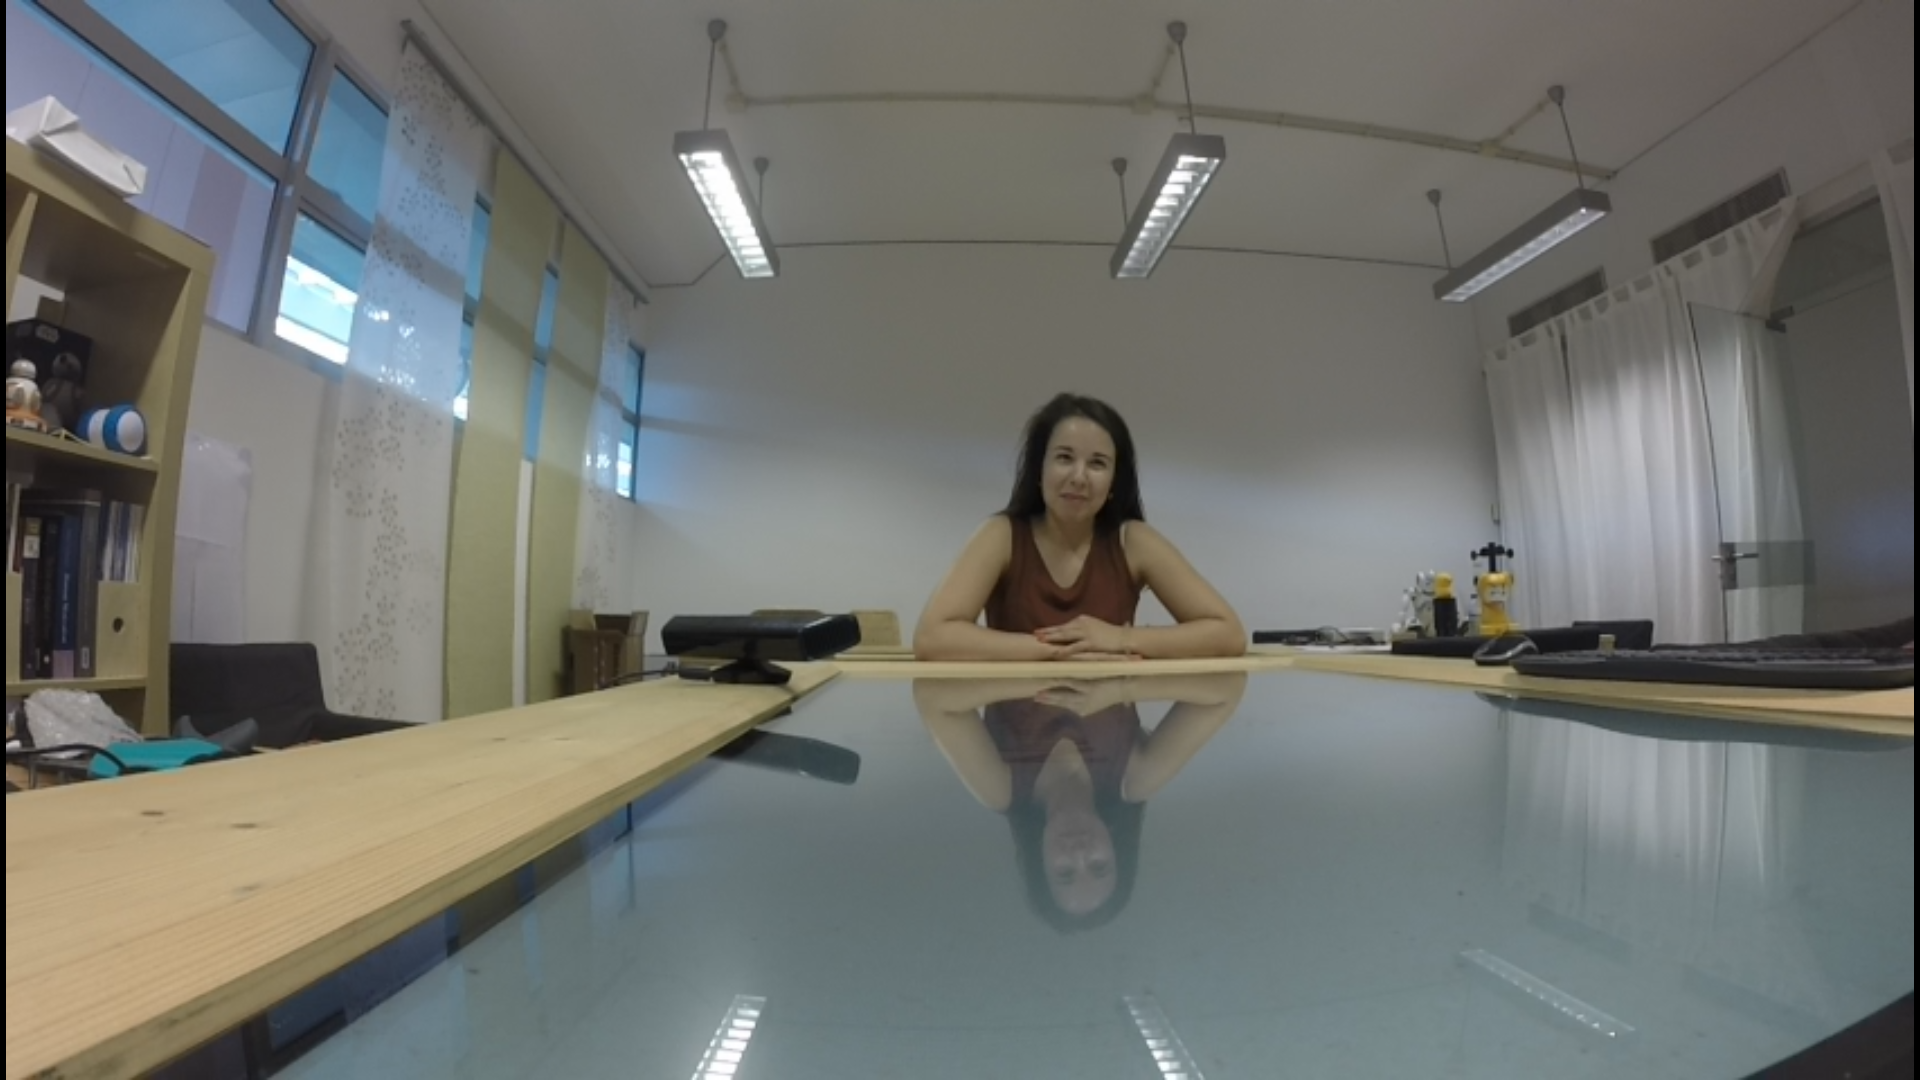
\includegraphics[width=0.7\textwidth]{images/CloseupScenario.png}}
	\caption{An example of a participation in the Quick Numbers study (frontal view).}
	\label{fig:quickNumbersScenarioCloseup}
\end{figure}

To conclude, we strongly believe that low sample size ($n=20$) and the design of the scenario were the main culprit. On one hand, with a increased sample size, the patterns might have confirmed the hypotheses with a significance lower than 5\%. And, on the other hand, the scenario should have provided more opportunities to build rapport, as even in the existing opportunities, participants were more focused on the task, and not on the agent as intended which made them less attentive to the agent's attempts to manage rapport hindering the results of the experiment. In addition, previous experience with the robot \ac{EMYS} might have the impacted on the results, as there were already attempts to build rapport in the past, with or without success. In order to reduce the impact of previous experience, the scenario should have considered different utterances considered that some participants already interacted with the partner in the past, for example, the agent might comment ``Your face is not strange to me, we already played some games in the past, didn't we?'' if the participant already interacted with \ac{EMYS} previously. This way, we are discerning between building rapport (participants who never played with \ac{EMYS} with managing rapport (participants who already played with \ac{EMYS} in the past).
\cleardoublepage

%Chapter 7
\fancychapter{Conclusions}
\label{chap:conclusions}

This dissertation addresses the development of a rapport model that enables robotic and virtual agents to show natural signs of rapport according to the dyadic state of the interaction. This work was inspired by current literature on rapport~\cite{Buschmeier2011, Spencer-Oatey2005, Zhao2014, Papangelis2014} and social agents~\cite{Zwiers2011, Reidsma2011, Riek2009, Niewiadomski2009, Andrist2014, Andrist2015, Cassell2007, Wang2009, Schroder2010, Buschmeier2011, Tullio2015}.

The main difficulties during the development of this dissertation were:
\begin{itemize}
	\item Gathering and organising current research on rapport and social agents onto a consistent computational model;
	\item Developing the framework that implements rapport model while maintaining compatibility with current \ac{SERA} agents;
	\item Integration of \ac{SSI}, SHORE, and GRETA with the developed framework;
	\item Designing the tools to assure that current researchers may start using the developed system.
\end{itemize}

The model is based on the development of decoupled rapport strategies that can be refined and customised individually, to any agent and \ac{HRI} scenario. The model was integrated using the \ac{SERA} ecosystem and tested using robot \ac{EMYS}, however, we had to create a framework within \ac{SERA} to support interruption and replacement of the agent's ongoing actions as required in the rapport model. The goal of the framework is to provide technical and non-technical researchers, the tools to design agents capable of showing signs of rapport. Several efforts were made so that the system maintained compatibility with \ac{SERA}, be customisable, and work with external tools such as \ac{SSI}, SHORE and GRETA thanks to the collaboration of Fraunhofer Institute for Integrated Circuits (IIS) and TELECOM ParisTech university. In fact, current \ac{SERA} agents can use the developed rapport model with low effort.

To conclude, there were no relevant conclusions from the Quick Numbers user studies regarding likeability, perceived intelligence, liveness and proximity. However, from the video footage, it was clear that participants had more positive reactions on the rapport condition than on the control condition. For this purpose, it is possible to retrieve additional behavioural metrics from the recorded video (total 1235 minutes) to analyse, for example, smile frequency and length of eye contact. In addition, from the histograms, despite the lack of statistically significant results on the obtained results, there is a clear pattern that rapport strategies can make the agents more likeable as intended, which may be confirmed by repeating the studies with a sample greater than 20.




%TODO escarrapachar as dificuldades?

\section{Contributions}
\label{sec:contributions}

This dissertation contributed to:
\begin{itemize}
    \item Design of a rapport model that enables robotic and virtual agents to show natural signs of rapport according to the dyadic state of the interaction;
    \item Construction of a framework that implements the rapport model and eases the development of rapport agents by technical and non-technical researchers;
    \item Integration of \ac{SSI}, SHORE and SEMAINE with the \ac{SERA} ecosystem using the developed framework as intermediary;
    \item Development of a novel scenario called Quick Numbers, to evaluate rapport and trust;
    \item User studies that evaluate a rapport agent using robot \ac{EMYS} regarding participant perception of likeability, animacy, intelligence and felt proximity.
\end{itemize}

\section{Future Work}

This section presents several ideas that can be implemented in the future, to improve the work developed so far.

First of all, we need to evaluate the system on a different scenario focused on rapport, not on trust with a greater sample. This would aim to shift the participant's focus from the game to the agents, which has impacted the reported results in this document. In addition, we should look into behavioural metrics such as eye contact and smile frequency.

Secondly, future versions of the rapport model should consider mechanisms to assess rapport success so that the agent might adapt his behaviours to the user and even recover from mistakes~\cite{Kahn2008}. For example, use SHORE to monitor the emotional state of the user and attempt use humour to cheer him as soon as sadness becomes the most average emotion. In addition, we should continue collaboration with Fraunhofer Institute for Integrated Circuits (IIS) so that we can continuously improve the rapport model and the system using the SHORE's perceptual capabilities. For example, estimate the user gender to automatically select the most appropriate set of utterances.

Thirdly, we should explore resumable actions, that is, explore agents capable of resuming their course of action after being interrupted by external stimuli.

Finally, the backchannel \textit{Effector} should be revisited as it is only lacking an improved noise suppressing mechanism. This plugin has the potential to greatly enhance mutual attention and coordination that are two of the three components of rapport. Looking ahead, this \textit{Effector} should explore current \ac{ML} models to generate listener behaviour, as the current literature suggests that data models are the key to generating more humanly social behaviours.
\cleardoublepage

%%%%%%%%%%%%%%%%%%%%%%%%%%%%%%%%%%%%%%%%%%%%%%%%%

%%%%%%%%%%%%%%%%%%%%%%%%%%%%%%%%%%%%%%%%%%%%%%%%%
% BIBLIOGRAPHY
% Add the Bibliography to the PDF table of contents (not the document table of contents)
\pdfbookmark[0]{Bibliography}{bib}
% The bibliography style sheet
% Chose your preferences on the format of the entries and the Labels:

% IEEEtran: Used in general (recommended for IST Thesis)
%           Entries are labelled and sorted by appearance in the document
%           Labels are Numeric inside square brackets
% \bibliographystyle{IEEEtran}

% Apalike:  Entries formatted alphabetically, last name first, with identation
%           Labels with Autor's Name and Year inside square brackets
% \bibliographystyle{apalike}

% Alpha:    Entries formatted with Autor's Name and Year, hanging identation
%           Labels with Autor's abbr. Names and Year inside square brackets
% \bibliographystyle{alpha}

% Acm:     Entries formatted with Autor's Name (small Caps), hanging identation
%          Labels are Numeric inside square brackets
\bibliographystyle{acm}
% The following command resets the 'emphasis' style for bibliography entries
\normalem
% Name of your BiBTeX file

\bibliography{Bibliography/IEEEabrv,Bibliography/library,Bibliography/questionnaires}
\ULforem
\cleardoublepage
%%%%%%%%%%%%%%%%%%%%%%%%%%%%%%%%%%%%%%%%%%%%%%%%%


%%%%%%%%%%%%%%%%%%%%%%%%%%%%%%%%%%%%%%%%%%%%%%%%%
% APPENDIX
\appendix

\chapter{Questionnaires used in User Studies}
\label{chapter:questionnaires}
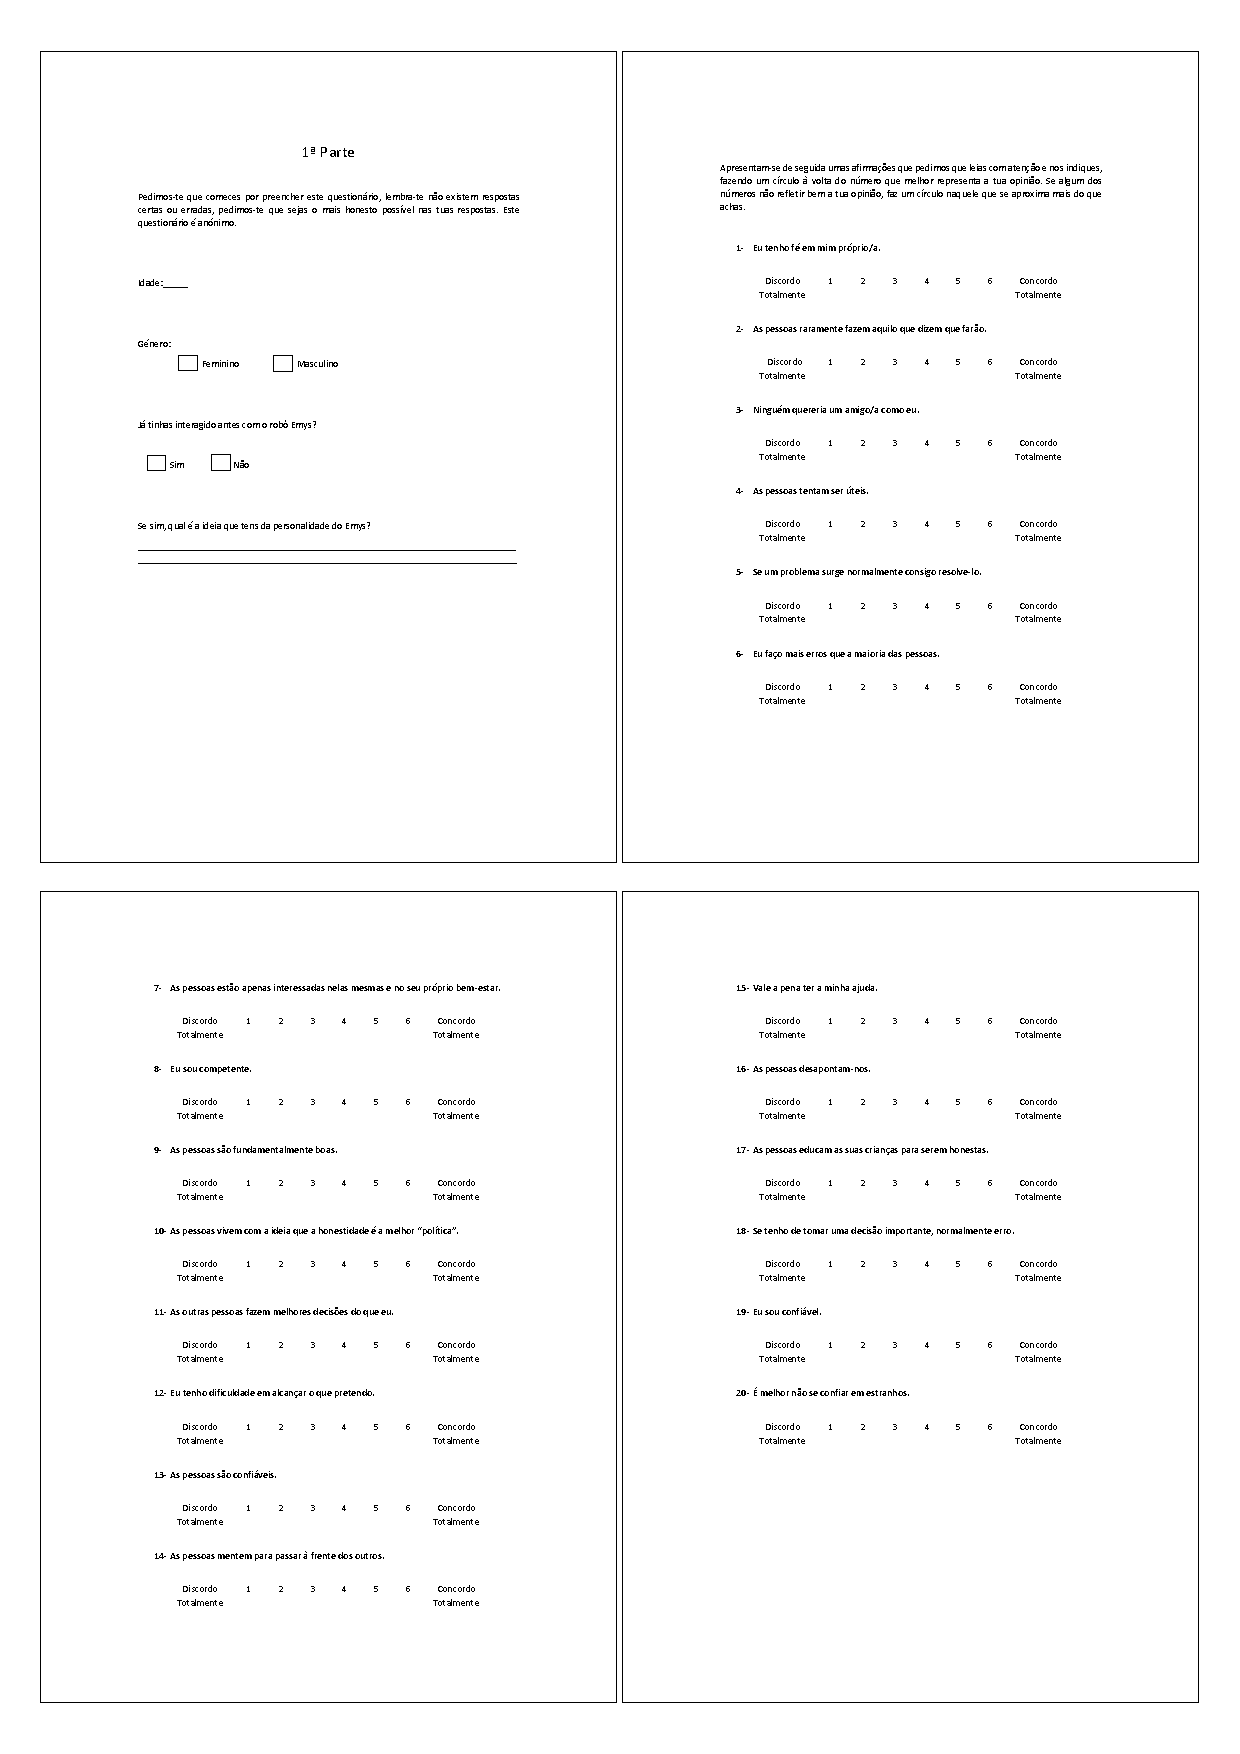
\includepdf[pages={-}]{external/questionarioCompressed.pdf}
%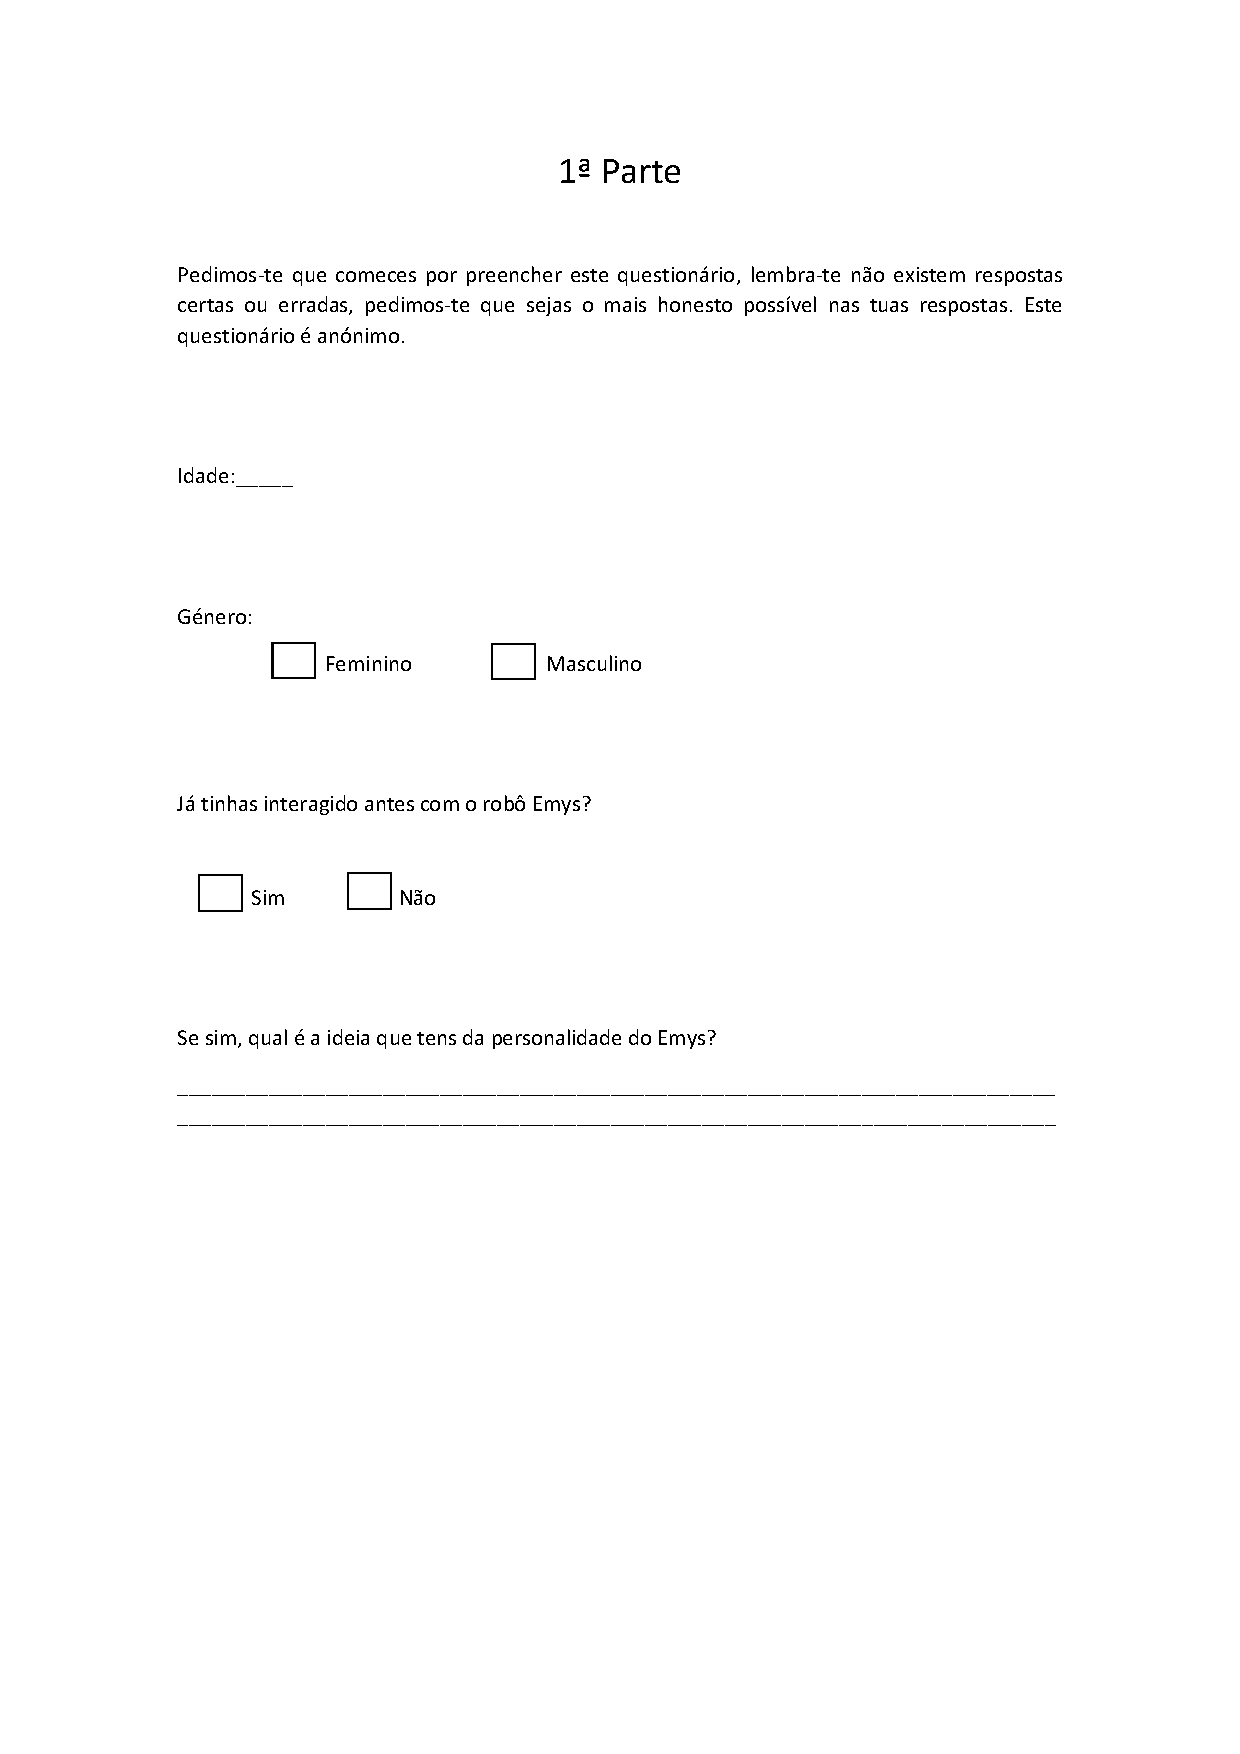
\includepdf[pages={-}]{external/questionario.pdf}
\cleardoublepage

\chapter{Example Configuration File}
\label{chapter:appendixB}

\vspace{9.5cm}


\begin{lstlisting}[caption={Excerpt of the Facial Expression Mimicry \textit{Effector} configuration file. The final animation is the \texttt{BaseAnimation} appended with a random number between 1 and 5, resulting on, for example, suprise3.},label={lst:facialExpressionsSettings},language=XML]
<MimicFacialExpressionsSettings>
  <MinimumMimicDelay>3500</MinimumMimicDelay>
  <Happy>
    <Probability>0.5</Probability>
    <MinimumIntensity>0.65</MinimumIntensity>
    <Priority>1</Priority>
    <BaseAnimation>joy</BaseAnimation>
  </Happy>
  <Sad>
    <Probability>0.5</Probability>
    <MinimumIntensity>0.65</MinimumIntensity>
    <Priority>1</Priority>
    <BaseAnimation>sadness</BaseAnimation>
  </Sad>
  <Surprised>
    <Probability>0.5</Probability>
    <MinimumIntensity>0.5</MinimumIntensity>
    <Priority>1</Priority>
    <BaseAnimation>surprise</BaseAnimation>
  </Surprised>
</MimicFacialExpressionsSettings>
\end{lstlisting}

\chapter{Example \textit{Effector} Plugin}

\vspace{9.5cm}

\begin{lstlisting}[language=CSharp, caption={Example definition of an \textit{Effector} Plugin that mimics facial expressions using event handlers.},classoffset=2,morekeywords={RenderState,PrimitiveRestart,FacetCulling,RasterizationMode,ScissorTest,StencilTest,DepthTest,DepthRange,Blending,ColorMask},label={lst:facialExpressionsSourceCode}]
using GRETAConnection;
using RapportActionProposer.ProposeStrategies;
using RapportActionProposer.RCPluginDefinition;
using RapportAgentPlugin;
using System;
using System.ComponentModel.Composition;

namespace MimicFacialExpressions {

    public class MimicFacialExpressionsSettings {
        public class ExpressionTriggerSetting {
            public double TriggerProbability { get; set; } = 0.48;
            public double MinimumIntensity { get; set; }
            public ushort Priority { get; set; }
            public string BaseAnimation { get; set; }
        }
        
        public int MinimumDelayMsBetweenActions { get; set; } = 3500;
        
        public ExpressionTriggerSetting Happy { get; set; } = new ExpressionTriggerSetting() 
            { MinimumIntensity = 0.65, Priority = 1, BaseAnimation = "joy" };

        public ExpressionTriggerSetting Sad { get; set; } = new ExpressionTriggerSetting() 
            { MinimumIntensity = 0.65, Priority = 1, BaseAnimation = "sadness"};

        public ExpressionTriggerSetting Surprised { get; set; } = new ExpressionTriggerSetting() 
            { MinimumIntensity = 0.5, Priority = 1, BaseAnimation="surprise" };
    }

    [Export(typeof(IRCPlugin))]
    [RCPluginMetadata(Description = "Mimics human emotions")]
    [EffectorMetadata(ProposalsManagementStrategy = ProposeStrategyType.OneActionGlobal)]
    public class MimicHumanFacialExpressions : EffectorPlugin<MimicFacialExpressionsSettings> {
        AgentActionsManager agent;
        Random random = new Random();
        GretaPerceptionReceiver gretaPerceptionsReceiver;

        public override void Init() {
            base.Init();
            (Operations.ProposeActionStrategy as OneActionGlobalProposeActionStrategy).MinimumTimeBetweenActionsMs = Settings.MinimumDelayMsBetweenActions;
        }

        public override void InitDependencies() {
            base.InitDependencies();

            agent = RapportController.GetPlugin<AgentActionsManager>();
            gretaPerceptionsReceiver = RapportController.GetPlugin<GretaPerceptionReceiver>();
        }

        public override void Start() {
            base.Start();

            if (gretaPerceptionsReceiver.gretaChannelReceiver == null) {
                throw new Exception("GretaPerceptionsReader must be initialized first!");
            }

            gretaPerceptionsReceiver.gretaChannelReceiver.HappyEvent += HumanIsHappy;
            gretaPerceptionsReceiver.gretaChannelReceiver.SadEvent += HumanIsSad;
            gretaPerceptionsReceiver.gretaChannelReceiver.SurpriseEvent += HumanIsSurprised;
        }

        public override void Pause() {
            base.Pause();

            if (gretaPerceptionsReceiver.gretaChannelReceiver == null) {
                throw new Exception("GretaPerceptionsReader must be initialised first!");
            }

            gretaPerceptionsReceiver.gretaChannelReceiver.HappyEvent -= HumanIsHappy;
            gretaPerceptionsReceiver.gretaChannelReceiver.SadEvent -= HumanIsSad;
            gretaPerceptionsReceiver.gretaChannelReceiver.SurpriseEvent -= HumanIsSurprised;
        }

        private double GetRandomNumber(double minimum, double maximum) {
            return random.NextDouble() * (maximum - minimum) + minimum;
        }

        public void HumanIsHappy(object sender, EmotionEventArgs e) {
            TriggerAux(e.Intensity, Settings.Happy);
        }

        public void HumanIsSad(object sender, EmotionEventArgs e) {
            TriggerAux(e.Intensity, Settings.Sad);
        }

        public void HumanIsSurprised(object sender, EmotionEventArgs e) {
            TriggerAux(e.Intensity, Settings.Surprised);
        }

        public void TriggerAux(double intensity, MimicFacialExpressionsSettings.ExpressionTriggerSetting expression) {
            if (intensity >= expression.MinimumIntensity && expression.TriggerProbability >= GetRandomNumber(0, 1)) {

                string animation = expression.BaseAnimation + random.Next(1, 6).ToString();

                var proposal = agent.Actions.Animate(animation, expression.Priority, 0, 30000);
                ProposeAction(proposal);
            }
        }
    }
}
\end{lstlisting}


\chapter{User Studies Utterances}
\label{chapter:appendixC}

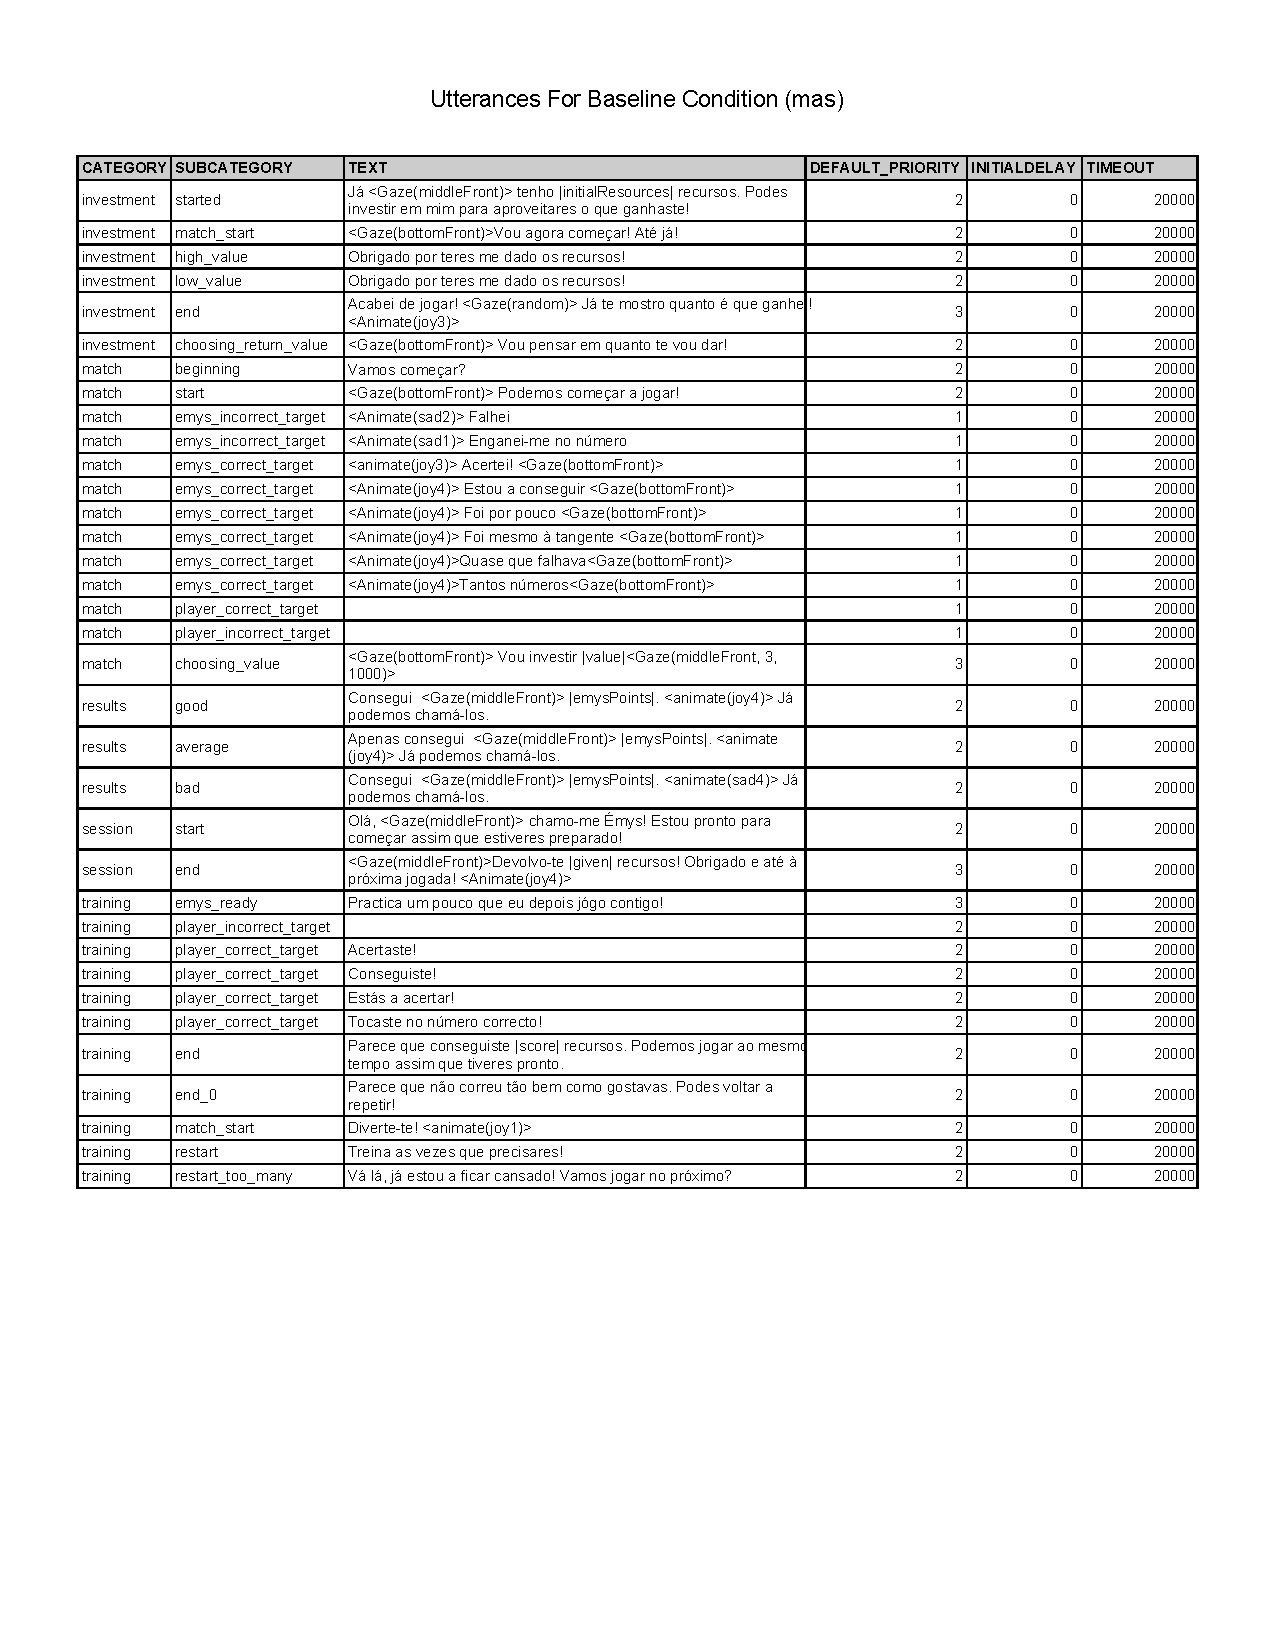
\includepdf[pages={-}]{external/UTTERANCES_BASELINE_mas.pdf}
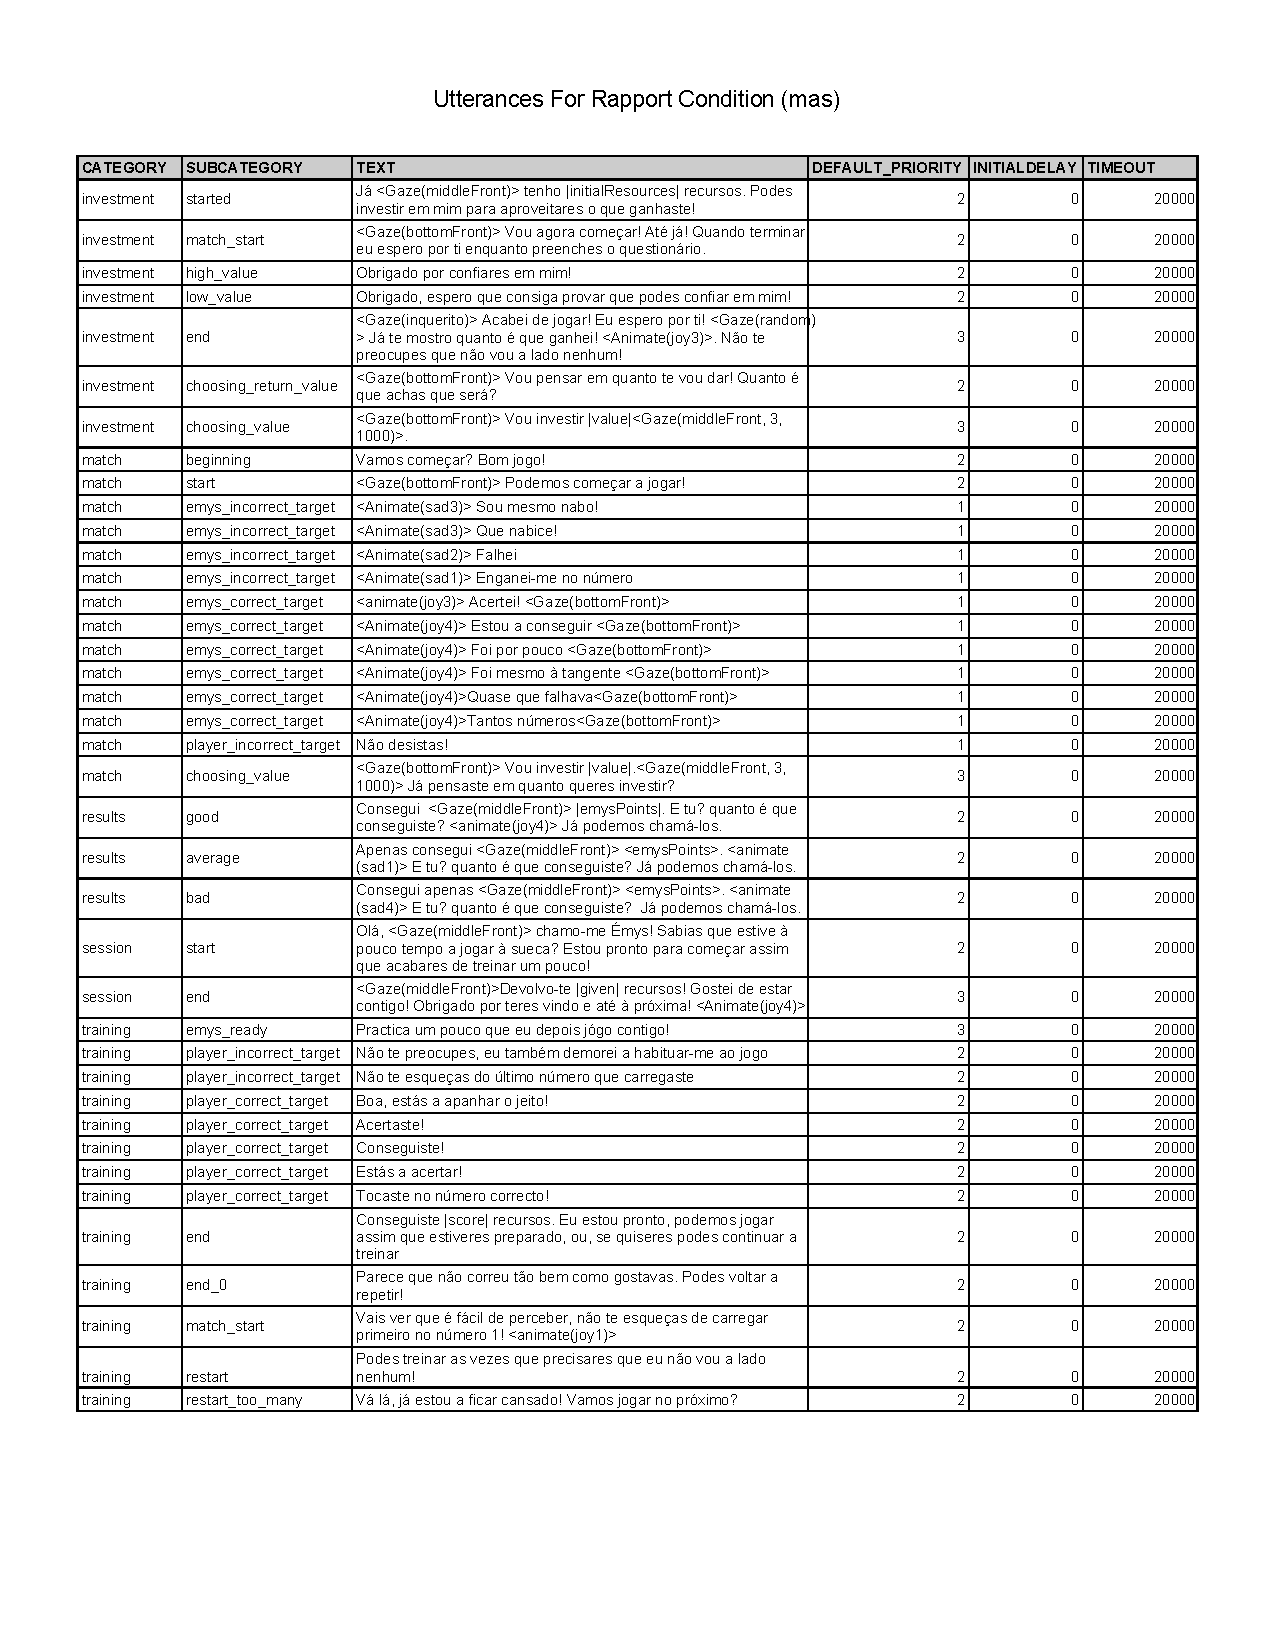
\includepdf[pages={-}]{external/UTTERANCES_RAPPORT_mas.pdf}

\clearpage
%\cleardoublepage
%%%%%%%%%%%%%%%%%%%%%%%%%%%%%%%%%%%%%%%%%%%%%%%%%

\end{document}